%%%%%%%%%%%%%%%%%%%%%%%%%%%%%%%%%%%%%%%%%%%%%%%%%%%%%%%%%%
% Formattazione base del documento con supporto caratteri
% accentati da tastiera win/linux e lingua italiana
%%%%%%%%%%%%%%%%%%%%%%%%%%%%%%%%%%%%%%%%%%%%%%%%%%%%%%%%%%

\documentclass[12pt,a4paper,oneside,openright]{book}
%modifico l'interlinea
\linespread{1.3}

\usepackage[latin1]{inputenc}
\usepackage[italian]{babel}
\usepackage{verbatim}
%%%%%%%%%%%%%%%%%%%%%%%%%%%%%%%%%%%%%%%%%%%%%%%%%%%%%%%%%%%%
% Pacchetto per il controllo della sintassi
% Decommentare \syntaxonly
%%%%%%%%%%%%%%%%%%%%%%%%%%%%%%%%%%%%%%%%%%%%%%%%%%%%%%%%%%

\usepackage{syntonly}
\usepackage{textcomp}
%\usepackage{dsfont}
% \syntaxonly

%%%%%%%%%%%%%%%%%%%%%%%%%%%%%%%%%%%%%%%%%%%%%%%%%%%%%%%%%%
% Inclusione pacchetto per la gestione delle figure che
% andranno copiate nella cartella figure
%
% Esempio di uso: avendo un file di nome figura1.eps questa
% si inserisce nella tesi con il comando:
%
% \begin{figure}[ht]
% \begin{center}
% \includegraphics{figura1.eps}
% \caption[nome breve]{nome lungo}
% \end{center}
% \end{figure}
%
% Il nome breve è quello che apparirà nell'indice delle
% figure ed è opzionale.
% Il nome lungo è quello che appare sotto la figura.
%%%%%%%%%%%%%%%%%%%%%%%%%%%%%%%%%%%%%%%%%%%%%%%%%%%%%%%%%%

\usepackage[final]{graphicx}
%\graphicspath{{./images/}}
\DeclareGraphicsExtensions{.png,.pdf,.jpg}

% evita il warning di pdllatex riguardo alle immagini pdf
% con versione 1.5 (al massimo 1.4 era di default..)
\pdfoptionpdfminorversion=5

% small 
\usepackage[font=small]{caption}

%\usepackage{subfigure}
%\usepackage{wrapfig}



%%%%%%%%%%%%%%%%%%%%%%%%%%%%%%%%%%%%%%%%%%%%%%%%%%%%%%%%%%
% Inclusione pacchetto per la generazione automatica
% dell'indice analitico.  Per esempio se vogliamo che la
% parola "raggruppamenti" sia indicizzata nella frase
% "I raggruppamenti sono realizzati per..." si dovrà
% scrivere "i raggruppamenti\index{raggruppamenti} ..."
%
% Compilando il file, il LaTeX produrrà un file ausiliario
% che termina con ".idx". Bisogna far processare questo
% file idx dal programma ausiliario "bibtex", che produrrâ
% a sua volta un altro file ancora. Dare infine un'ultima
% passata col LaTeX. Si può tranquillamente lasciare la
% compilazione dell'indice verso la fine della stesura del
% lavoro, quando tutto è ormai quasi definitivo.
%%%%%%%%%%%%%%%%%%%%%%%%%%%%%%%%%%%%%%%%%%%%%%%%%%%%%%%%%%

%\usepackage{makeidx}
%\usepackage{tocbibind}
%\makeindex

%%%%%%%%%%%%%%%%%%%%%%%%%%%%%%%%%%%%%%%%%%%%%%%%%%%%%%%%%%
% Numerazione delle sessioni fino alle subsub e inclusione
% nell'indice
%%%%%%%%%%%%%%%%%%%%%%%%%%%%%%%%%%%%%%%%%%%%%%%%%%%%%%%%%%

%\setcounter{secnumdepth}{4}
\setcounter{tocdepth}{4}

%%%%%%%%%%%%%%%%%%%%%%%%%%%%%%%%%%%%%%%%%%%%%%%%%%%%%%%%%%
% Inclusione pacchetto per la gestione della impostazioni
% personalizzate per la prima pagina
%%%%%%%%%%%%%%%%%%%%%%%%%%%%%%%%%%%%%%%%%%%%%%%%%%%%%%%%%%

\usepackage{unipr}
    \titolo{Titolo Italiano}
    \titoloIng{English Title}
    \laureando{Alex Spagni}
    \annoaccademico{2021-2022}
    \corsodilaurea{Ingegneria Informatica, Elettronica e Telecomunicazioni}
    \relatore[Prof.]{Relatore Michele Amoretti} 
    \correlatorea[Ing.]{Nome Correlatore 1} 
    \correlatoreb[Ing.]{Nome Correlatore 2 (opzionale)}

    %\citazione{\textit{\textquotedblleft Se ho visto più lontano, \`e perch\`e stavo sulle spalle di giganti.\textquotedblright \\ Isaac Newton}}

%%%%%%%%%%%%%%%%%%%%%%%%%%%%%%%%%%%%%%%%%%%%%%%%%%%%%%%%%%
% utilizzo il pacchetto fancyhdr per l'header e il footer
%%%%%%%%%%%%%%%%%%%%%%%%%%%%%%%%%%%%%%%%%%%%%%%%%%%%%%%%%%

\usepackage{fancyhdr}


 % Package aggiunti
  \usepackage{amssymb}				% matematica
  \usepackage{amsmath}				% matematica
  \usepackage{amsthm}				% matematica -> stile teoremi, def, proposizioni
  \usepackage{amsbsy}				% for bold math symbol
  \usepackage{cases}				% sistemi di equazioni con numerazione e sottonumerazione
  \usepackage{booktabs}				% tabelle con toprule ecc
  \usepackage{textcomp}				% per il simbolo di gradi
  \usepackage{subfig}				% per mettere pi figure in una stessa
  \usepackage{longtable}
  \usepackage[chapter]{algorithm}	% per mettere l'ambiente flottante attorno all'algoritmo (chapter \`e per la numerazione)
  \usepackage{algorithmic}			% per creare algoritmi
  \floatname{algorithm}{Algoritmo}					% opzioni dell'algoritmo: titolo in italiano
  \renewcommand{\algorithmicrequire}{\textbf{Input:}}		% require->input
  \renewcommand{\algorithmicensure}{\textbf{Output:}}	% ensure->output
  %\setlength{\parindent}{0in}			% per togliere l'indentazione all'inizio di un nuovo paragrafo

%%%%%%%%%%%%%%%%%%%%%%%%%%%%%%%%%%%%%%%%%%%%%%%%%%%%%%%%%%
% utilizzo il pacchetto hyperref per i link nel pdf, oltretutto setto i colori dei link a nero
% nota: funziona solo con pdfLatex
%%%%%%%%%%%%%%%%%%%%%%%%%%%%%%%%%%%%%%%%%%%%%%%%%%%%%%%%%%

\usepackage[pdftex,colorlinks,plainpages=false,hyperindex,bookmarksopen,linkcolor=black,citecolor=black,urlcolor=black]{hyperref}
% pacchetto per creare i link con pdfLatex
%\usepackag{hyperref}
%\hypersetup{colorlinks=true, linkcolor=black, urlcolor=black}

%%%%%%%%%%%%%%%%%%%%%%%%%%%%%%%%%%%%%%%%%%%%%%%%%%%%%%%%%%
% Comandi aggiuntivi
%%%%%%%%%%%%%%%%%%%%%%%%%%%%%%%%%%%%%%%%%%%%%%%%%%%%%%%%%%
%\newcommand{\EQ}[1]{Eq.~(\ref{#1})}
%\newcommand{\BEGMATRIX}[1]{\left[\begin{array}{#1}}
%\newcommand{\ENDMATRIX}{\end{array}\right]}
%\def\argmin{\mathop{\rm argmin}}

%%%%%%%%%%%%%%%%%%%%%%%%%%%%%%%%%%%%%%%%%%%%%%%%%%%%%%%%%%
% Corpo della tesi
%%%%%%%%%%%%%%%%%%%%%%%%%%%%%%%%%%%%%%%%%%%%%%%%%%%%%%%%%%

\begin{document}

% PAGE HEADERS permette di creare gli header delle pagine con il numero, il capitolo e la riga sotto
\pagestyle{fancy}
\headheight 15pt
\renewcommand{\chaptermark}[1]{\markboth{{\chaptername}\ \thechapter.\hspace{1em}#1}{}}
\renewcommand{\footrulewidth}{0pt}
% definisce l'header e il footer
\lhead[\fancyplain{}{}]{\fancyplain{}{\leftmark}} \chead{}
\rhead{\thepage} \lfoot{} \cfoot{} \rfoot{}

% definizione dei teoremi, proposizioni, definizioni ecc usato con il package amsthm
\newtheorem{definizione}{Definizione}[chapter] 		% il chapter si usa per la sotto numerazione nei capitoli
\newtheorem{proposizione}{Proposizione}[chapter]
\newtheorem{problema}{Problema}[chapter]
\newtheorem{proprieta}{Propriet\`a}[chapter]


%%%%%%%%%%%%%%%%%%%%%%%%%%%%%%%%%%%%%%%%%%%%%%%%%%%%%%%%%%
% Inizio della parte introduttiva
%%%%%%%%%%%%%%%%%%%%%%%%%%%%%%%%%%%%%%%%%%%%%%%%%%%%%%%%%%
\maketitle


\frontmatter
\pagenumbering{alph}



\chapter*{Ringraziamenti}



\pagenumbering{roman}
\tableofcontents
%\listoffigures


%\lstlistoflistings


%%%%%%%%%%%%%%%%%%%%%%%%%%%%%%%%%%%%%%%%%%%%%%%%%%%%%%%%%%
% Inizio della parte centrale
%%%%%%%%%%%%%%%%%%%%%%%%%%%%%%%%%%%%%%%%%%%%%%%%%%%%%%%%%%
% \pagenumbering{arabic}
\mainmatter

\chapter*{Introduzione} % \chapter* -> the introduction isn't the Chapter 1, it's not a numbered chapter
\addcontentsline{toc}{chapter}{Introduzione} %this line enable the introduction to be listed in the Table Of Contents even if it's not a numbered chapter (see above)
\markboth{}{}


\clearpage
\chapter{Stato dell'arte}
All'giorno d'oggi siamo costantemente influenzati dal mondo mobile, quindi viene spontaneo chiedersi quali sono le possibili strade da seguire per poter sviluppare un'app.
Innanzitutto \`e necessario fare una distinzione tra app nativa e app multipiattaforma.
Le prime sono delle applicazioni software che sono state sviluppate per funzionare su uno
specifico tipo di dispositivo o piattaforma. Invece la seconda \`e un applicazione che pu\`o essere eseguita anche su sistemi operativi differenti ma usando sempre lo stesso codice.
In particolare un app nativa sviluppata per un dispositivo Android non funzionar\`a su dispositivi iOS e viceversa un app sviluppata
per un dispositivo iOS non funzioner\`a su dispositivi Android \cite{ReactNativeCLI:Expo} \cite{app:ibride:native}.\\

%\section{Sviluppo mobile}
\section{App Multipiattaforma}
React native \`e un Framework per lo sviluppo di app multipiattaforma che permette di sviluppare applicazioni sia per Android che iOS.
Per poter utilizzare questo Framework esistono due principali ``strumenti": Expo\cite{ReactNativeCLI:Expo} e React Native CLI\cite{ReactNativeCLI:Expo}.
Entrambi mettono a disposizione una serie di servizi per aiutare nello sviluppo. In particolare Expo \`e un Framework che estende React Native
\subsection{React Native}
\begin{figure}[h]
      \centering
      
\includegraphics[width=5cm, height=4cm]{images/ReactNativeLogo-NoBackground.png}
      \caption[differenzeiteot]{}
      \label{fig:ReactNative}
\end{figure}

In React Native, proprio come in React, vengono costruiti dei componenti JSX, i quali combinano markup e il JavaScript, che lo controlla, in un unico file. A differenza del web non
si ha una separazione tra grafica, presentazione e controllo in file diversi, in quanto JSX privilegia la separazione delle ``concern" rispetto alla
separazione delle tecnologie.

Il ciclo di aggiornamento \`e lo stesso di React: quando le "props"  o gli "state" cambiano, React Native esegue un nuovo rendering delle viste.\\
La differenza principale tra React Native e React nel browser \`e che React Native sfrutta le librerie dell'interfaccia utente, della sua piattaforma ospitante,
anzich\`e utilizzare il markup HTML e CSS.

React Native CLI permette di utilizzare React Native per sviluppare diversi tipi di applicazioni, tra cui:
\begin{itemize}
      \item Prototipi
      \item Applicazioni multipiattaforma
      \item Applicazioni che non fanno largo uso di API native
      \item Applicazioni con una complessa User Interface {}(UI)
      \item Applicazioni per un determinato sistema operativo
      \item Applicazioni che non fanno uso intensivo di animazioni
\end{itemize}
Tra i vari vantaggi derivanti dall'utilizzo di questo ``strumento", bisogna sottolineare che:
\begin{list}{*}{}
      \item Permette di includere moduli nativi scritti in Java, Kotlin e Object-C
      \item Consente di ridurre i tempi di sviluppo, in quanto permette di riutilizzare gran parte del codice scritto per le applicazioni web
      \item Mette a disposizione un gran numero di componenti pre-costruiti
      \item Fornisce un interfaccia utente semplice
      \item Permette di utilizzare plugin di terze parti
      \item Consente di realizzare una migliore User Interface rispetto ad Expo
      \item Presenta un architettura modulare la quale consente di semplificare lo sviluppo, il test e la manutenzione di programmi di grosse dimensioni
\end{list}
Mentre tra i vari svantaggi, si ha che:
\begin{list}{*}{}
      \item Per poter effettuare i test \`e necessario collegare il dispositivo al Pc
      \item Richiede Android Studio e XCode per l'esecuzione dei progetti
      \item Per poter condividere la propria app \`e necessario condividere l'intero file .apk
      \item La preparazione di un progetto richiedere tempo e non \`e cos\`i  semplice come con Expo
      \item Richiede una conoscenza preliminare della strutturazione delle cartelle in Android e iOS
\end{list}

Una volta installata un'applicazione sviluppata in React Native sul proprio dispositivo, questa non eseguir\`a il render nel browser DOM, anzi andr\`a ad invocare le Object-C APIs, per eseguire il render su dispositivi IOS,
e andr\`a ad invocare le Java APIs, per eseguire il render su dispositivi Android. L'utilizzo di tali API \`e possibile grazie al ``bridge", il quale fornisce a React un'interfaccia con gli elementi
della UI nativa della piattaforma ospitante.\\ In particolare i "React component" restituiscono il markup della loro funzione di rendering,
il quale descrive il loro aspetto. Quando si utilizza React, per lo sviluppo web, questo si traduce direttamente nel DOM del broswer. Per React Native, il markup di un componente viene tradotto per adattarsi alla piattaforma host.
Quindi una $<$View$>$ potrebbe diventare una UIView specifica per iOS \cite{ReactNative} \cite{ReactNativeCLI:Expo}.

\begin{figure}[h]
      \centering
      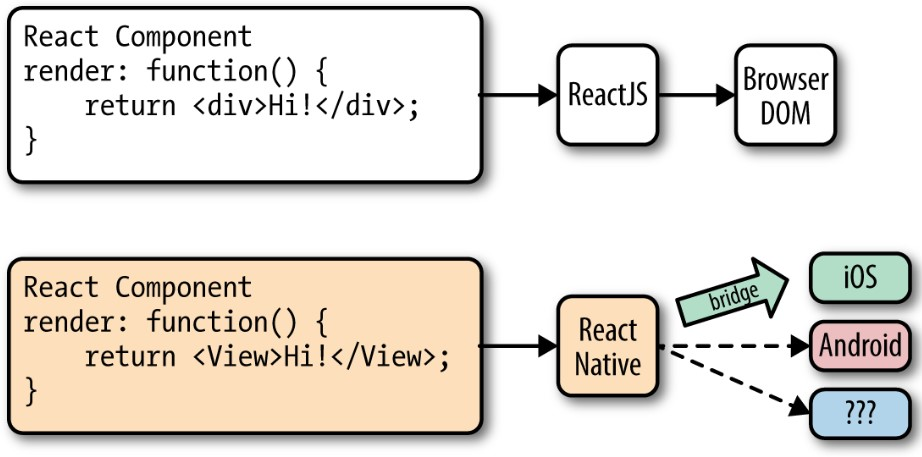
\includegraphics[width=10cm, height=4cm]{images/ReactRendering.jpg}
      \caption[differenzeiteot]{}
      \label{fig:ReactRendering}
\end{figure}


\subsection{Expo}
Expo \`e simile a React Native CLI, ma con uno svantaggio considerevole. In alcune applicazioni \`e necessario
accedere alle API native che non sono disponibili su Javascript, per esempio le API per accedere ad Apple e Google play.
In altri casi all'interno di un'applicazione si
potrebbe voler riutilizzare le librerie scritte in Java, Object-C,Swift,Kotling o C++ che non sono state implementate in Javascript.

I moduli nativi permettono di esporre
delle istanze di classi Java, Object-C e C++ come oggetti JavaScript. In questo modo \`e possibile eseguire codice nativo in JavaScript.\\
Expo non permette di utilizzare i moduli nativi, quindi a meno che una certa libreria non sia gi\`a stata implementata in JavaScript, questa non potr\`a essere utilizzata
in un'applicazione sviluppata tramite Expo.
Questo non \`e l'unico svantaggio derivante dall'utilizzo di questo strumento. Alcune device API non sono supportate, come ad esempio il bluetooth.\\
A parte questo Expo presenta diversi vantaggi, tra cui \cite{ReactNative:Sito} \cite{ReactNativeCLI:Expo}:
\begin{list}{*}{}
      \item Una migliore gestione dei link
      \item Mette a disposizione una maggiore quantit\`a di librerie standart, come ad esempio una libreria per le "Push Notification"
      \item Offre una migliore "Development Experience". Per poter testare un'applicazione, sviluppata tramite Expo, non \`e necessario avere un emulatore del dispositivo, su cui la si vuole testare, o collegare il proprio dispositivo al pc
            Expo permette di testare le applicazioni tramite Wi-fi, collegando il dispositivo e il pc alla stessa rete LAN
      \item Le applicazioni vengono aggiornate pi\`u velocemente rispetto a React Native CLI
      \item Supporta "l'Over to air update", quindi un applicazione si aggiorna nel momento in cui quest'ultima si sta aprendo sul dispositivo su cui \`e installata
      \item Non \`e necessario effettuare la build dell'applicazione per poterla testare
      \item \`E possibile "espellere" il progetto in ExpoKit e integrare del codice nativo, continuando ad utilizzare alcune funzionalit\`a di Expo, ma non tutte
\end{list}

\subsection{React Navigation}
Sia che si utilizzi Expo o React Native CLI, aspetti molto importanti nello sviluppo di un'app sono la presentazione e la navigazione tra i vari ``Screen". Quest'ultimi
rappresentano la parte di User Interface con la quale l'utente interagir\`a. La navigazione tra i vari screen
viene gestita da un ``Navigator". Il principale Navigator utilizzato sia da Expo che da React Native si chiama ``React Navigation".
Questa \`e una standalone library che permette di gestire lo spostamento tra i vari screen di cui l'applicazione \`e composta.

React Navigation fornisce principalmente quattro Navigator\cite{ReactNavigation}, ognuno dei quali consente ad un utente di passare da uno screen ad un altro:
\begin{itemize}
      \item Native Stack Navigator: Ogni volta che un utente effettua una transizione
            il nuovo screen viene messo in cima allo stack. Il Native Stack Navigator utilizza le API native UINavigationController per le applicazione sviluppate per iOS e le API native Fragment per le
            applicazioni sviluppate per Android. \\In questo modo la navigazione tra i vari screen avr\`a lo stesso comportamento e le stesse prestazioni
            di applicazioni che usano la navigazione nativa. Nonostante le prestazioni fornite da questo Navigator siano ottime, non \`e particolarmente "customizzabile"
            come lo Stack Navigator.
      \item Stack Navigator: A differenza del Native Stack Navigator questo \`e incredilmente "customizzabile", poich\`e implementato in Javascript. Nonostante ci\`o non usando le primitive di navigazione native
            presenta prestazioni peggiori. Va comunque detto che per la maggior parte delle applicazioni questa differenza di performance tra il Native Stack Navigator e lo Stack Navigator non \`e percebile.
      \item Drawer Navigator: La differenza principale tra questo Navigator e gli altri \`e che quest'ultimo viene rappresentato con un icona formato da tre linee orizzontali, posta in alto a sinistra della visualizzazione. Attraverso
            quest'ultima \`e possibile vedere tutti gli screen su cui si pu\`o navigare.
      \item Tab Navigator: Questo Navigator viene rappresentato tramite una Tab-Bar posta nella parte bassa dello schermo. Essa mostra gli screen verso cui si
            pu\`o navigare. Questo Navigator \`e uno dei pi\`u utilizzati nelle applicazioni basate su Tab-Bar.
\end{itemize}


\subsection{Redux}

Al giorno d'oggi le single-page application devono gestire sempre pi\`u stati, ed \`e per questo che nella maggior parte delle app
si utilizza Redux. Questa \`e una libreria molto leggera che aiuta a sviluppare applicazioni che si comportano in modo coerente, che vengono eseguite in
ambienti diversi (client e server) e che sono facili da testare. Si dice che Redux permetta di realizzare un ``contenitore a stato" prevedibile, per le applicazioni JavasScript.

Questa libreria \`e completamente compatibile con React Native, attraverso l'utilizzo di React Redux, il quale rappresenta il livello di binding ufficiale di React UI per Redux.
Questo livello consente ai "React component" di leggere i dati da un archivio e di inviare azioni a quest'ultimo per aggiornarne lo stato.\\
In particolare, Redux:
\begin{itemize}
      \item Permette di realizzare uno store che contiene lo stato globale
      \item Consente di emettere azioni che aggiornano lo stato dello store. Queste vengono notificate all'archivio nel momento in cui avviene un evento nell'applicazione
      \item Presenta delle funzioni riduttrici pure che esaminano le azioni e restituiscono uno stato immutabile aggiornato
\end{itemize}
Quando si parla di ``stati" da gestire all'interno di un'app, si fa riferimento, ad esempio: alle risposte di un server, a dati salvati nella
cache o creati locamente e che non sono memorizzati in modo persistente. Redux \`e in grado di gestire tutti questi stati e permette di rendere la mutazione
dello stato globale prevedibile, attraverso l'imposizione di alcune restrizioni, su quando e come lo stato pu\`o essere modificato.

Queste restrizioni possono essere riassunte nei tre principi cardine di Redux\cite{Redux}:

\begin{enumerate}
      \item Lo stato globale dell'applicazione \`e memorizzato in un albero di oggetti all'interno di un singolo store. In questo modo \`e possibile realizzare app universali, permettere un miglior debugging dell'applicazione e
            rendere lo stato globale persistente in modo da avere un ciclo di sviluppo pi\`u rapido.
      \item Lo stato \`e Read Only. Questo assicura che n\'e le ``viste" n\'e le callback di rete scrivano direttamente sullo stato. Al contrario, esprimono l'intenzione di trasformare lo stato.
            \\Dato che tutte le modifiche sono centralizzate e avvengono una alla volta in un ordine rigoroso, non vi sono condizioni di concorrenza a cui dover prestare attenzione.
            Le azioni per aggiornare lo stato sono semplici oggetti JavaScript, quindi possono essere registrate, serializzate, memorizzate e successivamente riprodotte per scopi
            di debug o di test.
      \item Lo stato viene aggiornato da funzioni pure, le quali sono chiamate riduttori. Queste prendono lo stato precendete, un'azione e restituiscono lo stato successivo.
            In particolare i riduttori devono ritornare nuovi oggetti di stato e non modificare lo stato precendente.

\end{enumerate}

%\subsubsection{React Native}
%\subsubsection{Expo}
\section{App Native}

Come gi\`a menzionato all'inizio di questo capitolo, le applicazioni native sono sviluppate per uno specifico dispositivo o piattaforma ed \`e quindi necessario un linguaggio di programmazione differente da un sistema operativo all'altro.
iOS fa uso dei linguaggi Object-C e Swift, mentre Android sviluppa app native in Java e Kotlin.
\subsection{Kotlin}

Kotlin \`e un linguaggio sviluppato da JetBrains a partire dal 2010 e successivamente reso open source nel 2012. \`E definito come general purpose, free, open source e pragmatico. Pragmatico in quanto cerca di distinguersi dalla struttura chiusa e ben
definita di Java al fine di permettere uno sviluppo pi\`u snello e veloce, grazie soprattutto al fatto che fornisce diversi ``shortcut".

Koltin nel 2019 \`e diventato, secondo Google, il linguaggio pi\`u utilizzato per lo sviluppo di applicazioni Android, sostituendo Java \cite{KotlinTech}.
Nonostante lo si utilizzi per lo sviluppo di applicazioni Android native, quest'ultimo permette anche la realizzazione di applicazioni per iOS e di applicazioni web, in quanto \`e possibile transpilare il codice scritto in Kotlin
in codice JavaScript \cite{Kotlin:JetBrains}.
%Oltre ad essere utilizzato per lo sviluppo front-end, quindi lato client, pu\`o essere utilizzato anche per lo sviluppo backend. In particolare Kotlin pu\`o lavorare con diverse tecnologie lato server, come WebGL o Node.js.\\

Kotlin consente di realizzare applicazioni seguendo il paradigma Object Oriented {}(OOP) o il paradima della programmazione funzionale. Nel primo caso si fa uso delle classi, dell'ereditariet\`a e del polimorfismo, proprio come in Java.
Nel secondo caso il programma si basa sulla valutazione di funzioni matematiche. In questo modo \`e possibile ottenere il meglio dei due mondi\cite{KotlinInfoWorld}.

Un ambiente di esecuzione per le applicazioni scritte tramite questo linguaggio, \`e la JVM {}(Java Virtual Machine). Questo ambiente di esecuzione consente di utilizzare Kotlin in
qualsiasi contesto in cui viene utilizzato Java. Inoltre, Kotlin \`e al 100\% interoperabile con quest'ultimo. Il vantaggio di questo alto livello di interoperabilt\`a \`e che si possono riutilizzare le librerie Java esistenti\cite{kotlin}.

Kotlin e Java sono molto simili tra loro, ed entrambi possono essere utilizzati per lo sviluppo di applicazioni per Android. Nonostante ci\`o presentano alcune differenze\cite{KotlinBaeldung}:
\begin{itemize}
      \item Il codice scritto in Kotlin risulta essere pi\`u conciso di quello scritto in Java, in quanto riduce la quantit\`a di "BoilerPlate".
      \item Un'applicazione sviluppata in Kotlin risulta essere pi\`u facile da leggere e presenta meno errori dovuti allo sviluppatore.
      \item Java consente di assegnare ad una variabile il valore "Null", il quale pu\`o generare un errore "NullPointerException", nel caso in cui la variabile venisse acceduta.\\ Invece
            Kotlin applica la cosiddetta "Null Safety", cio\`e non permette di assegnare ad una variabile il valore "Null". In questo modo il codice risulta essere pi\`u stabile.
      \item Kotlin non \`e un linguaggio fortemente tipizzato come invece lo \`e Java. Infatti vengono utilizzate solo due parole chiave per la definizione delle variabili. Inoltre, solo nel momento in cui ad una variabile viene assegnato un valore, questa viene
            identificata come una stringa, un numero o un booleano. Lo stesso meccanismo ricorre anche in JavaScript.
      \item Una differenza fondamentale tra i due \`e che Java supporta solo la programmazione ad oggetti, mentre invece Kotlin oltre a quest'ultima supporta anche la programmazione funzionale.
      \item Java presenta un tempo di compilazione inferiore rispetto a Kotlin. Nel caso di piccole applicazioni si stima che Java sia il 15-20\% pi\`u veloce rispetto
            al tempo necessario per compilare la stessa applicazione scritta in Kotlin. Se per\`o consideriamo app di dimensioni maggiori, allora il tempo di compilazione \`e circa lo stesso.

\end{itemize}

Secondo alcuni studi solo i neofiti dello sviluppo Android continuano a sviluppare applicazioni in Java, poich\'e la maggior parte
della documentazione e degli esempi sono in Java.\\
Altri studi dimostrano che il tempo medio impiegato da uno sviluppatore Java per imparare Kotlin \`e di poche ore. Dopo questa transizione si stima una riduzione del 40\% del numero di linee di codice da Java a Kotlin\cite{KotlinInfoWorld}.\\
\subsection{Swift}
Swift \`e un potente linguaggio di programmazione che permette di creare applicazioni sia per dispotivi mobili come cellulari,
IPad e Apple Watch, ma anche per dispositivi come Mac e Apple Tv.
Essendo un linguaggio general-purpose, proprio come Kotlin, pu\`o essere usato anche per sviluppare applicazioni web e web service. Inoltre, \`e possibile realizzare applicazioni server che
necessitano di "runtime security" e ingombro di memoria ridotto.

Swift \`e stato realizzzato per essere un linguaggio veloce. Utilizzando la tecnologia di compilazione LLVM il codice Swift viene trasformato in codice macchina ottimizzato che sfrutta al meglio
l'hardware moderno.

Questo linguaggio di programmazione \`e il successore dei linguaggi C e Object-C, in quanto include sia primitive di basso livello come tipi,
controllo di flusso e operatori ma fornisce anche funzionalit\`a orientate agli oggetti come classi, protocolli e i tipi generici.
Swift ha eliminato intere classi di codice ``non sicuro". Le variabili devono sempre essere inizializzate prima di essere utilizzate, gli indici degli array e gli interi
vengono sempre controllati per verificare se vi sono errori di overflow \cite{Apple:Com}.

Questo linguaggio presenta diverse caratteristiche, tra cui\cite{Apple:Swift}:
\begin{itemize}
      \item Supporta i tipi generici
      \item Le funzioni possono ritornare valori multipli e tuple
      \item Presenta un iterazione rapida e concisa su un intervallo o un insieme
      \item Presenta modelli di programmazione funzionale, ad esempio ``map" e ``filter"
      \item Presenta una gestione degli errori integrata.
\end{itemize}

Tramite Swift la memoria viene gestita automaticamente utilizzando l'ARC {}(Automatic Reference Counting). Esso permette di mantenere l'utilizzo della
memoria al minimo e senza l'onere del Garbage Collection \cite{GarbageCollector}. Si ricorda che in Java, il Garbage Collection si occupa di tenere traccia delle allocazioni di memoria utilizzate e le
libera solo quando non sono pi\`u impiegate. Esso \`e un vero e proprio thread in esecuzione parallelamente al programma e anche se la sua priorit\`a
\`e minima, quindi viene avviato solo quando non ci sono altri thread attivi, \`e  un processo da considerare in termini di tempo di CPU.

Swift \`e open source e cross-platform infatti pu\`o essere usato sia su piattaforme Apple che Linux. Presenta anche un package manager, il quale \`e un
unico strumento multipiattaforma per costruire, eseguire, testare e pacchetizare le librerie e gli eseguibili Swift. Swift Package Manager stesso \`e costruito con Swift
e incluso nel progetto Open Source Swift come pacchetto.

Tramite Questo linguaggio \`e possibile creare una nuova applicazione oppure utilizzare il codice Swift per implementare nuove caratteristiche e funzionalit\`a nelle proprie applicazioni.
Il codice Swift coesiste con i file Object-C esistenti nello stesso progetto, con pieno accesso alle API Object-C\cite{Apple:Com}.\\
Anche se Swift \`e interoperabile con Object-C, esso presenta alcuni vantaggi rispetto a quest'ultimo\cite{Swift:ObjectC}:
\begin{list}{*}{}
      \item Secondo Apple Swift pu\`o essere 2.6 volte pi\`u veloce di Object-C
      \item In Swift possono essere create delle variabili senza doverne definire prima il tipo
      \item Non \`e necessario inserire i punti e virgola alla fine di ogni riga di codice scritta in Swift
      \item Il codice scritto in Swift viene scirtto pi\`u velocemente rispetto al codice scritto in Object-C, poich\`e Swift \`e stato
            progettato per essere "Developer-Friendly"
\end{list}

\subsection{Swift vs Kotlin}
Sia Kotlin che Swift sono linguaggi di programmazione che vengono usati per lo sviluppo di app native, ed entrambi sono multipiattaforma.
Nonostante ci\`o presentano alcune differenze, di seguito elencate\cite{Swift:Kotlin}:
\begin{itemize}
      \item Lo sviluppo in Kotlin non si limita ad un particolare IDE o OS. Infatti \`e possibile scrivere il proprio codice Kotlin in qualsiasi IDE o OS come VS Code, Atom, Windows, Linux e Mac.\\
            Al contrario lo sviluppo in Swift \`e possibile solo all'interno di XCode perch\'e solo attraverso di esso si \`e in grado di compilare il codice Swift
            Questo IDE \`e disponibile solo su Mac, quindi non sar\`a possibile sviluppare app per IOS senza averne uno
      \item Kotlin e Swift approcciano la gestione della memoria in modo differente. In particolare Kotlin, proprio come Java, affronta la gestione di quest'ultima dal punto di vista del Garbage Collection.\\
            All'contrario Swift fa uso dell'ARC {}(Automatic Reference Counting). Attraverso di esso le applicazioni sviluppate tramite Swift tendono ad essere pi\`u efficienti e prive di bug
      \item Entrambi, all'interno di un progetto possono coesistere con i rispettivi predecessori. Swift \`e al 100\% interoperabile con Object-C, mentre Kotlin \`e al 100\% interoperabile con Java
\end{itemize}
Una caratteristica comune ad entrambi \`e che permettono di ridurre la quantit\`a di "BoilerPlate", necessaria sia nei progetti Java che in quelli Object-C.

\section{App Native vs App Multipiattaforma}
Quando si decide di sviluppare un'applicazione per un dispositivo mobile, come pu\`o essere un telefono, \`e necessario capire se si vuole sviluppare un'app nativa o un'app multipiattaforma.
La scelta pu\`o essere fatta sulla base di cinque fattori: prestazioni, tempo di sviluppo, sicurezza, User Experience/Interface e stabilit\`a\cite{NativeApp:MultiplatformApp}.

Per fornire le massime prestazioni agli utenti, la scelta pi\`u saggia che si pu\`o fare \`e scegliere un approccio nativo, poich\'e
le app native sono sviluppate tenendo conto dei requisiti specifici della piattaforma di riferimento. Esse sono compilate per una specifica serie di dispositivi ed
eseguite per una precisa architettura. Ci\`o che consente alle app native di essere pi\`u efficienti \`e l'accesso ad API e componenti esclusivi, ottimizzati per diverse dimensioni di schermo e versioni di sistema.
Questa tipologia di app pu\`o presentare dimensioni minori rispetto alle app multipiattaforma, consentendo di occupare meno memoria sul dispositivo.

Per quanto riguarda i tempi di sviluppo, le app multipiattaforma presentano uno produzione pi\`u rapida. Grazie alla riusabilit\`a del codice tra le piattaforme, un gruppo di sviluppatori
non necessita di implementare progetti separati per sistemi operativi diversi.

Dal punto di vista della sicurezza, le app native sono pi\`u sicure rispetto alle app multipiattaforma, poich\'e sono dotate di molteplici funzioni di sicurezza incorporate.
Per gli sviluppatori di applicazioni native \`e solitamente pi\`u facile implementare la crittografia dei file, il rilevamento inteligente delle frodi e altre
funzioni di sicurezza attraverso le opportune librerie e risorse di ogni piattaforma.\\
L'aggiornamento delle misure di sicurezza nelle app native richiede meno tempo rispetto alle app multipiattaforma. In quest'ultime \`e pi\`u difficile prevedere quando i framework multipiattaforma saranno aggiornati.

Se l'obiettivo \`e quello di realizzare la miglior User Experience o User Interface per la propria applicazione, allora \`e necessario privilegiare un approccio nativo. Le applicazioni native offrono migliori funzionalit\`a
dell'interfaccia utente, poich\'e dispongono di librerie e componenti preimpostati e personalizzabili.

Se l'intento \`e quello di sviluppare un applicazione stabile nel lungo tempo, allora bisogna adottare un approccio nativo. Dato che Android e IOS provengono rispettivamente da Google e Apple,
\`e certo che queste aziende continueranno a supportare e migliorare i loro sistemi operativi mobili. Questo significa che le app native beneficeranno di stabilit\`a in termini di manutenzione e aggiornamenti.\\
D'altra parte, dato che i framework multipiattaforma sono creati da aziende, organizzatori e comunit\`a di sviluppatori di terze parti, c'\`e il rischio che l'aggiornamento o lo sviluppo di questi
framework possa essere incoerente o interrotto.






\chapter{Specifica Funzionale del Sistema Realizzato}
\section{Obiettivi dell'Applicativo}
Lo scopo principale dell'applicativo sviluppato \`e quello di fornire un servizio per la visualizzazione delle immagini scattate dai diversi Rover inviati su Marte nel corso degli ultimi anni.
Queste immagini possono essere visualizzate sul proprio dispositivo mobile con sistema operativo Android o iOS, tramite una applicazione che pu\`o essere scaricata da un sito web online.

L'applicazione deve fornire una funzione di ricerca, tramite la quale si potranno ricercare immagini inserendo il nome di uno dei Rover oppure digitando la data solare in cui sono state scattate le immagini che si vogliono osservare. In particolare, i nomi dei Rover per i quali si potr\`a effettuare una ricerca sono: Curiosity, Spirit e Opportunity.
Tra una ricerca e l'altra verr\`a mostrata una schermata di ``loading" in modo da indicare all'utente che si sta eseguendo il ``fetching" delle immagini.

Oltre a poter ricercare le immagini secondo diversi parametri, l'applicazione deve anche fornire la possibilit\`a di nascondere alcune di queste in modo che non vengano visualizzate dall'utente in una ricerca futura.
Nonostante le immagini nascoste non vengano presentate all'utente quando effettua una ricerca, gli verr\`a sempre concessa la possibilit\`a di ripristinarle.

L'utente potrebbe non essere interessato ad un'intera categoria di immagini, quindi gli verr\`a fornita la possibilit\`a di nascondere tutte le foto relative ad una sua ricerca.

Ogni volta che verr\`a chiusa l'applicazione, le ultime immagini visualizzate dovranno essere memorizzata in modo persistente cos\`i che possano essere mostrate all'ultilizzatore quando riaprir\`a l'app.

Oltre a poter visualizzare le immagini in una lunga lista nell'Index Screen dell'applicazione, quest'ultima deve fornire anche la possibilit\`a di visualizzare i dettagli di ognuna di esse.

Al primo avvio l'utente dovr\`a essere ridirezionato verso una schermata di login o di registrazione a seconda che sia in possesso o meno delle credenziali di accesso.

\section{Requisiti dell'Applicativo}
\subsection{Requisiti Necessari per il Funzionamento dell'Applicativo}

L'applicazione necessita di una connessione ad Internet in modo da collegarsi
tramite il web ai server della Nasa e recuperare le immagini ricercate da ogni utente.

%Ogni utente la prima volta che accede all'applicazione o quando effettua il ``logout" da essa, deve inserire le proprie credenziali in modo da poter accedere all'Index Screen.\\
Le credenziali di ogni utente sono memorizzate in un database distribuito che memorizza i dati in documenti flessibili JSON-like. In particolare, per assicurare la sicurezza di ogni utilizzatore, le password di ognuno di essi vengono memorizzate
solo dopo essere state cifrate. In questo modo anche se qualcuno dovesse penetrare nel database non riuscirebbe ad accedere ai vari account.

Il database viene consultato attraverso un server locale che espone delle API all'applicativo per far s\`i che ogni utente possa eseguire la registrazione e il login.
Affinch\'e l'applicazione possa comunicare con il server locale, deve essere attiva un'applicazione Multipiattaforma chiamata Ngrok\footnote{Ngrok consente di aprire una connessione diretta verso le API sviluppate in Express e fornisce un URL tramite il quale il dispositivo mobile pu\`o usufruirne. In particolare, espone le porte su cui i server locali sono in ascolto ad Internet.}.


Per garantire l'efficienza dell'applicazione il numero di immagini recuperate, ad ogni richiesta GET ai server della Nasa, deve essere pari a 25. In questo modo si evita di sovraccaricare il client che deve elaborare le immagini e presentarle a schermo.

In Fig 2.1 si pu\`o osservare una rappresentazione grafica dell'interazione tra i vari sistemi:
\begin{figure}[h]
    \centering
    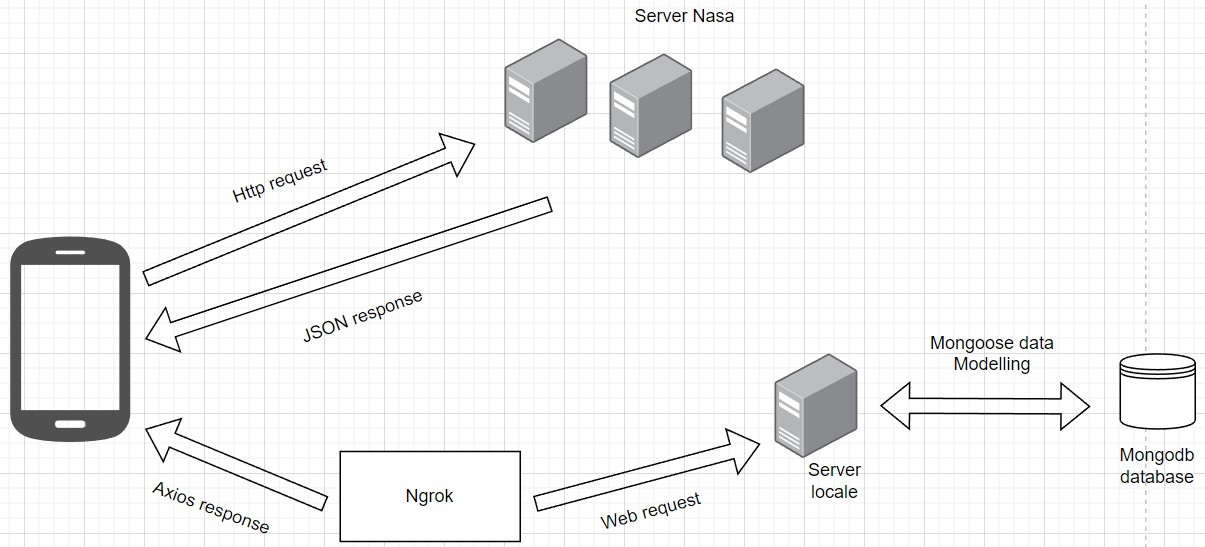
\includegraphics[width=13cm, height=7cm]{images/ModelloDiComunicazioneApplicazione.jpg}
    \caption[differenzeiteot]{Comuncazone tra i vari sistemi costituenti l'applicazione}
    \label{fig:modellodicomunicazione}
\end{figure}
\subsection{Requisiti funzionali}

Ad ogni requisito viene associato un nome mnemonico, una breve descrizione e un codice di priorit\`a in modo tale da indicare quali requisiti devono essere implementati per primi e quindi definire una gerarchia di implementazione.
\begin{center}
    \begin{longtable}{ | l | p{7cm} | l | }
        \hline
        \textbf{Nome}      & \textbf{Descrizione }                                                                                                     & \textbf{Priorit\`a} \\ \hline
        Sign in            & L'utente deve poter accedere all'applicazione tramite le sue credenziali                                                  & Primario            \\ \hline
        Sign up            & L'utente deve potersi registrare tramite la propria e-mail e password in modo da poter accedere all'applicazione          & Primario            \\ \hline
        Search by name     & L'utente deve poter ricercare le immagini tramite il nome di uno dei tre possibili Rover: Spirit, Opportunity e Curiosity & Primario            \\ \hline
        Search by date     & L'utente deve poter ricercare le immagini che sono state scattate in una precisa data solare                              & Primario            \\ \hline
        Hide image         & L'utente deve poter nascondere le immagini che gli vengono presentate                                                     & Primario            \\ \hline
        Restore images     & L'utente deve poter ripristinare le immagini che ha nascosto                                                              & Secondario          \\ \hline
        Logout             & L'utente deve poter uscire dal proprio profilo                                                                            & Secondario          \\ \hline
        Hide all           & L'utente deve poter nascondere nascondere tutte le ommagini relative ad una sua ricerca                                   & Secondario          \\ \hline
        Privacy and Policy & L'utente deve poter conoscere quali condizioni e termini ha accettato scaricando l'applicazione                           & Secondario          \\ \hline
    \end{longtable}
\end{center}
\subsection{Requisiti non funzionali}
In questa sezione vengono descritti i principali requisiti non funzionali necessari per il buon funzionamento dell'applicazione.
\begin{center}
    \begin{longtable}{ | l | p{7cm} | }
        \hline
        \textbf{Nome}    & \textbf{Descrizione }                                                                                                       \\ \hline
        Prestazioni      & L'applicativo deve essere in grado di presentare le immagini entro 6 secondi dall'avvio della ricerca                       \\ \hline
        Portabilit\`a    & L'applicativo deve poter essere scaricabile sia su dispositivi iOS che Android                                              \\ \hline
        Manutenibilit\`a & L'applicativo deve essere strutturato seguendo un architettura modulare in modo da facilitare la fase di test e di modifica \\ \hline
    \end{longtable}
\end{center}

\section{Casi d'Uso}

In questa sezione vengono illustrati i pricipali casi d'uso.%In ognuno di essi gli attori\footnote{L'attore \`e qualsiasi entit\`a che svolge un ruolo in un dato sistema. Questo potrebbe essere una persona, un'organizzazione o un sistema esterno. } sono gli end users e il server locale.
\subsection*{Caso d'uso U1: Sign in}
\begin{itemize}
    \item  \textbf{Use case overview:} l'applicazione deve consentire agli utenti la possibilit\`a di poter accedere al proprio account.
    \item \textbf{Actors:} end user, server locale.
    \item \textbf{Triggers:} si preme sul pulsante ``Sign in".
    \item \textbf{Pre-Condition:} l'utente non deve aver gi\`a effettuato l'accesso all'applicazione oppure si deve trovare nell'Index Screen dove pu\`o effettuare il logout.
    \item \textbf{Post-condition:} si verr\`a indirizzati nell'Index Screen dell'applicazione.
    \item \textbf{Main Flow:} \begin{enumerate}
              \item L'utente ha appena terminato di scaricare l'applicazione e la apre, ritrovandosi come prima schermata lo ``Splash screen". Una volta premuto il pulsante ``Explore" viene reindirizzato sullo screen destinato al log in.
              \item Arrivato allo screen di log in l'utente inserisce la propria e-mail e password e preme sul pulsante ``Sign in".
              \item Viene inviata una richiesta al server locale che va a confrontare le credenziali inserite in precedenza con quelle presenti sul database per verificare che coincidano. In caso affermativo l'utente viene indirizzato sull'Index Screen.

          \end{enumerate}
    \item \textbf{Alternative Flow:}\begin{enumerate}
              \item L'utente si trova nell'Index Screen e sta scorrendo tutta la lista di immagini a lui presentate. Una volta arrivato alla fine della lista preme sul pulsante di ``logout".
              \item L'utente si ritrova nello screen riservato al log in dove inserisce la propria mail e password e preme sul pulsante ``Sign in".
              \item Viene inviata una richiesta al server locale che va a confrontare le credenziali inserite in precedenza con quelle presenti sul database per verificare che coincidano. In caso affermativo l'utente viene indirizzato sull'Index Screen.
          \end{enumerate}

    \item \textbf{Exception Flow:}\begin{enumerate}
              \item Una volta inserite le proprie credenziali viene inviata una richiesta al server locale che va a confrontare queste ultime con quelle presenti sul database.
              \item Le credenziali inserite dall'utente non sono corrette e gli viene presentato un messaggio di errore. \end{enumerate}
\end{itemize}
\subsection*{Caso d'uso U2: Sign up}
\begin{itemize}
    \item  \textbf{Use case overview:} l'applicazione deve consentire agli utenti la possibilit\`a di potersi registrare tramite la propria e-mail e password.
    \item \textbf{Actors:} end user, server locale.
    \item \textbf{Triggers:} si preme sul pulsante ``Sign up".
    \item \textbf{Pre-Condition:} l'utente non deve aver gi\`a effettuato l'accesso all'applicazione.
    \item \textbf{Post-condition:}si viene indirizzati nell'Index Screen dell'applicazione.
    \item \textbf{Main Flow:} \begin{enumerate}
              \item L'utente ha appena terminato di scaricare l'applicazione e la apre, ritrovandosi come prima schermata lo ``Splash screen". Una volta premuto il pulsante "Explore" viene reindirizzato sullo screen destinato al log in. Non avendo alcune credenziale valida l'utente deve premere sul pulsante "Sign up" in modo da essere reindirizzato nello schermo dedicato alla registrazione.
              \item Arrivato allo screen di registrazione l'utente inserisce la propria e-mail e password e preme sul pulsante ``Sign up".
              \item Viene inviata una richiesta al server locale che va a confrontare che l'e-mail inserita dall'utente non sia gi\`a presente nel database. In caso affermativo l'utente viene indirizzato sull'Index Screen.

          \end{enumerate}

    \item \textbf{Exception Flow:}\begin{enumerate}
              \item Una volta inserite le proprie credenziali verr\`a inviata una richiesta al server locale che andr\`a a confrontare che l'e-mail inserita dall'utente non sia gi\`a presente nel database.
              \item Esiste gi\`a un utente registrato con quella e-mail, quindi il sistema restituisce un messaggio di errore. \end{enumerate}
\end{itemize}
\subsection*{Caso d'uso U3: Ricerca immagini tramite nome Rover}
\begin{itemize}
    \item  \textbf{Use case overview:} l'applicazione deve consentire agli utenti di ricercare le immagini in base al nome del Rover.
    \item \textbf{Actors:} End user, server Nasa.
    \item \textbf{Triggers:} si digita il nome di uno dei tre Rover nella Search Bar e si preme ``fatto" sulla propria tastiera.
    \item \textbf{Pre-Condition:} l'utente deve aver effettuato l'accesso oppure essere in possesso di un JSON Web Token.
    \item \textbf{Post-condition:} vengono presentate delle nuove immagini o una modale che informa l'utente che nessuna immagine \`e stata trovata.
    \item \textbf{Main Flow:} \begin{enumerate}
              \item L'utente si trova nella schermata principale e digita il nome del Rover che ha scattato le immagini richieste. Per avviare la ricerca si deve premere sul pulsante ``All".
              \item Viene effettuata una richiesta HTTP verso i server della Nasa i quali rispondono con un oggetto JSON che contiene tutte le foto che sono state trovate.
              \item Le immagini ottenute vengono inserite all'interno di una lista e vengono visualizzate a schermo.

          \end{enumerate}
    \item \textbf{Alternative Flow:}\begin{enumerate}
              \item L'utente si trova nella schermata principale e digita il nome del Rover che ha scattato le immagini le immagini richieste. Per avviare la ricerca si dovr\`e premere sul pulsante ``All".
              \item Viene effettuata una richiesta HTTP verso i server della Nasa i quali rispondono con un oggetto JSON che contiene tutte le foto che sono state trovate.
              \item Il nome del Rover inserito non \`e corretto. L'utente viene informato che non \`e stata trovata alcuna foto e gli viene presentata una lista di immagini vuota.

          \end{enumerate}
\end{itemize}
\subsection*{Caso d'uso U4: Ricerca immagini per data solare}
\begin{itemize}
    \item  \textbf{Use case overview:} l'applicazione deve consentire agli utenti la possibilit\`a di ricercare le immagini in base a una certa data solare.
    \item \textbf{Actors:} end user, server Nasa.
    \item \textbf{Triggers:} si preme sul pulsante ``Search by date".
    \item \textbf{Pre-Condition:} l'utente deve aver effettuato l'accesso oppure essere in possesso di un JSON Web Token.
    \item \textbf{Post-condition:} vengono presentate delle nuove immagini o una modale che informa l'utente che nessuna immagine \`e stata trovata.
    \item \textbf{Main Flow:} \begin{enumerate}
              \item L'utente si trova nell'Index Screen e preme il pulsante ``Data" in modo da spostarsi nello schermo dedicato alla ricerca per data solare. Deve quindi inserire giorno, mese e anno delle foto che vuole ricercare.
              \item Viene effettuata una richiesta HTTP verso i server della Nasa i quali rispondono con un oggetto JSON che contiene tutte le foto che sono state trovate.
              \item Le immagini ottenute vengono inserite all'interno di una lista e vengono visualizzate a schermo.

          \end{enumerate}
    \item \textbf{Alternative Flow:}\begin{enumerate}
              \item L'utente si trova nell'Index Screen e preme il pulsante ``Data" in modo da spostarsi nello schermo dedicato alla ricerca per data solare. Deve quindi inserire giorno, mese e anno delle foto che vuole ricercare.
              \item Viene effettuata una richiesta HTTP verso i server della Nasa i quali rispondono con un oggetto JSON che contiene tutte le foto che sono state trovate.
              \item Nella data solare inserita dall'utente non \`e stata scattata alcuna foto. Si viene quindi informati che non sono state trovate immagini e quindi non viene presentata alcuna foto.

          \end{enumerate}
\end{itemize}

\subsection*{Caso d'uso U5: Nascondere un immagine}
\begin{itemize}
    \item  \textbf{Use case overview:} l'applicazione deve consentire agli utenti la possibilit\`a di nascondere le immagini mostrate in modo che non vengano visualizzate in futuro.
    \item \textbf{Actors:} end user.
    \item \textbf{Triggers:} si preme sul pulsante ``Hide this image".
    \item \textbf{Pre-Condition:} l'utente deve aver effettuato l'accesso oppure essere in possesso di un JSON Web Token.
    \item \textbf{Post-condition:} l'immagine selezionata verr\`a nascosta.
    \item \textbf{Main Flow:} \begin{enumerate}
              \item L'utente si trova nell'Index Screen e premendo su un'immagine accede ai dettagli di quest'ultima.
              \item Premendo sul tasto ``Hide this image" viene nascosta l'immagine in questione e viene notificato all'utente un messaggio di conferma. A questo punto si viene reindirizzati sull'Index Screen.\\ \\ \\

          \end{enumerate}
    \item \textbf{Alternative Flow:}\begin{enumerate}
              \item L'utente si trova nell'Index Screen e premendo su un'immagine accede ai dettagli di quest'ultima.
              \item L'utente decide di non nascondere l'immagine in questione e ritorna sull'Index Screen premendo l'icona con la ``X".

          \end{enumerate}
\end{itemize}

\subsection*{Caso d'uso U6: Ripristinare le immagini nascoste precedentemente}
\begin{itemize}
    \item  \textbf{Use case overview:} l'applicazione deve consentire agli utenti la possibilit\`a di vedere anche le immagini nascoste in precedenza.
    \item \textbf{Actors:} end user.
    \item \textbf{Triggers:} si preme sul pulsante ``Photos".
    \item \textbf{Pre-Condition:} l'utente deve aver effettuato l'accesso oppure essere in possesso di un JSON Web Token.
    \item \textbf{Post-condition:} in base ai parametri di ricerca impostati dall'utente verranno mostrate tutte le immagini, anche quelle nascoste.
    \item \textbf{Main Flow:} \begin{enumerate}
              \item L'utente si trova nell'Index Screen e preme il pulsante ``Photos" il quale passa dal colore grigio ad azzurro in modo da indicare che \`e stato abilitato.
              \item Oltre alle immagini che l'utente stava gi\`a visualizzando, vengono mostrate anche quelle che aveva nascosto in precedenza. In particolare vengono ripristinate solo le foto nascoste che soddisfano i criteri di ricerca dell'utente.
          \end{enumerate}
    \item \textbf{Alternative Flow:}\begin{enumerate}
              \item L'utente si trova nell'Index Screen e preme il pulsante ``Photos" il quale passa dal colore azzurro a grigio in modo da indicare che \`e stato disabilitato.
              \item Tutte le immagini che l'utente aveva nascosto in precedenza vengono nuovamente occultate. Ora l'utente vede solo le foto che soddisfano i suoi parametri di ricerca e che non sono state nascoste.

          \end{enumerate}
\end{itemize}

\chapter{Implementazione}
Successivamente alla definizione dei requisiti funzionali e non funzionali dell'applicazione e alla descrizione dei diversi casi d'uso che coinvologono l'utente e altri sistemi esterni, si passa all'implementazione vera e propria dell'applicativo.
\section{Struttura iniziale di un'Applicazione in React Native}
Come strumento per lo sviluppo dell'applicazione \`e stato usato Expo, il quale permette di creare un nuovo progetto tramite l'utilizzo di questo comando all'interno del proprio terminale:
\begin{itemize}
    \item npx create-expo-app my-app
\end{itemize}
Quando si vuole sviluppare un'applicazione in React Native \`e richiesto di seguire una ``gerarchia delle cartelle" gestita da Expo. Quando si utilizza il comando sopra indicato per la creazione di un nuovo progetto,
queste sono le cartelle e i file che vengono creati:
\begin{itemize}
    \item La cartella ``node modules" contiene tutte le dipendenze e i package necessari al funzionamento dell'applicazione. Ogni volta che viene installato un nuovo package realizzato da terze parti, lo si ritrova in tale cartella.
    \item Il file ``package.json" permette di tenere traccia delle varie dipendenze, indicando quale versione di ogni package deve essere scaricata.
    \item Il file ``App.js" contiene il primo componente che viene mostrato ogni volta che viene aperta l'applicazione.
    \item La cartella ``assets" contiene le immagini che verranno utilizzate all'interno dell'applicazione.
\end{itemize}
\begin{figure}[h]
    \centering
    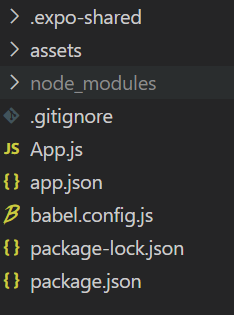
\includegraphics[width=5cm, height=7cm]{images/ExpoFileCartelle.png}
    \caption[differenzeiteot]{}
    \label{fig:ExpoCartelleFile}
\end{figure}
\section{Navigazione all'interno dell'Applicazione}
Ogni applicazione \`e composta da diversi screen ed \`e necessario permettere all'utente di transitare tra di essi. Per svolgere questa operazione \`e stata usata la
libreria \textit{React Navigation}, la quale fornisce diversi componenti e funzioni per la gestione della navigazione all'interno dell'app. In particolare all'interno
dell'applicativo ho utilizzati \cite{ReactNavigationContainer} \cite{ReactNavigationStackNavigator}:
\begin{itemize}
    \item NavigationContainer: \`e un componente responsabile della gestione dello stato dell'applicazione, del collegamento del top-level navigator all'ambiente dell'applicazione e dell'integrazione con la piattaforma specifica su cui verr\`a installata.
          Solitamente viene utilizzato una sola volta all'interno dell'applicativo e viene inserito nel file App.js/App.tsx. Lo scopo principale di questo componente \`e la gestione della navigazione tra i vari navigator che verranno inseriti all'interno dell'applicazione. Per poterlo utilizzare \`e necessario importarlo dalla libreria \textit{react-navigation}.
    \item Stack Navigator: fornisce all'applicazione la possibilit\`a di transitare attraverso gli screen e gestire la storia della navigazione. Ogni volta che l'utente transita da uno screeen ad un altro viene fatta un'operazione di ``push" e fa s\`i che il nuovo screen venga messo in cima allo stack. Invece, ogni volta che l'utente vuole tornare
          alla schermata precedente, viene fatta un'operazione di ``pop" e lo screen in cima allo stack viene rimosso. Per poterlo utilizzare \`e necessario importare la funzione ``createStackNavigator", la quale restituisce un oggetto che contiene due propriet\`a: \textit{Screen} e \textit{Navigator}.
          Entrambi sono dei ``React component" che vengono utilizzati per configurare il navigator. Il \textit{Navigator} permette di definire la route iniziale, ossia lo screen da mostrare per primo ogni volta che viene invocato lo Stack Navigator; questo componente dovr\`a contenere i vari \textit{Screen} i quali consentono di definire i vari schermi verso cui l'utente pu\`o transitare.
          Lo \textit{Screen} presenta 3 prop:
          \begin{list}{*}{}
              \item Name: il nome della route.
              \item Component: il JSX component da mostrare.
              \item Option: un oggetto che definisce alcune propriet\`a con cui lo schermo dovr\`a essere presentato.
          \end{list}
\end{itemize}
Tramite l'utilizzo della libreria {}(\textit{React Navigation}) \`e possibile annidare pi\`u navigator in modo da definire una gerarchia. L'importante \`e che in cima ad essa si abbia il NavigationContainer.\\
\begin{figure}[h]
    \centering
    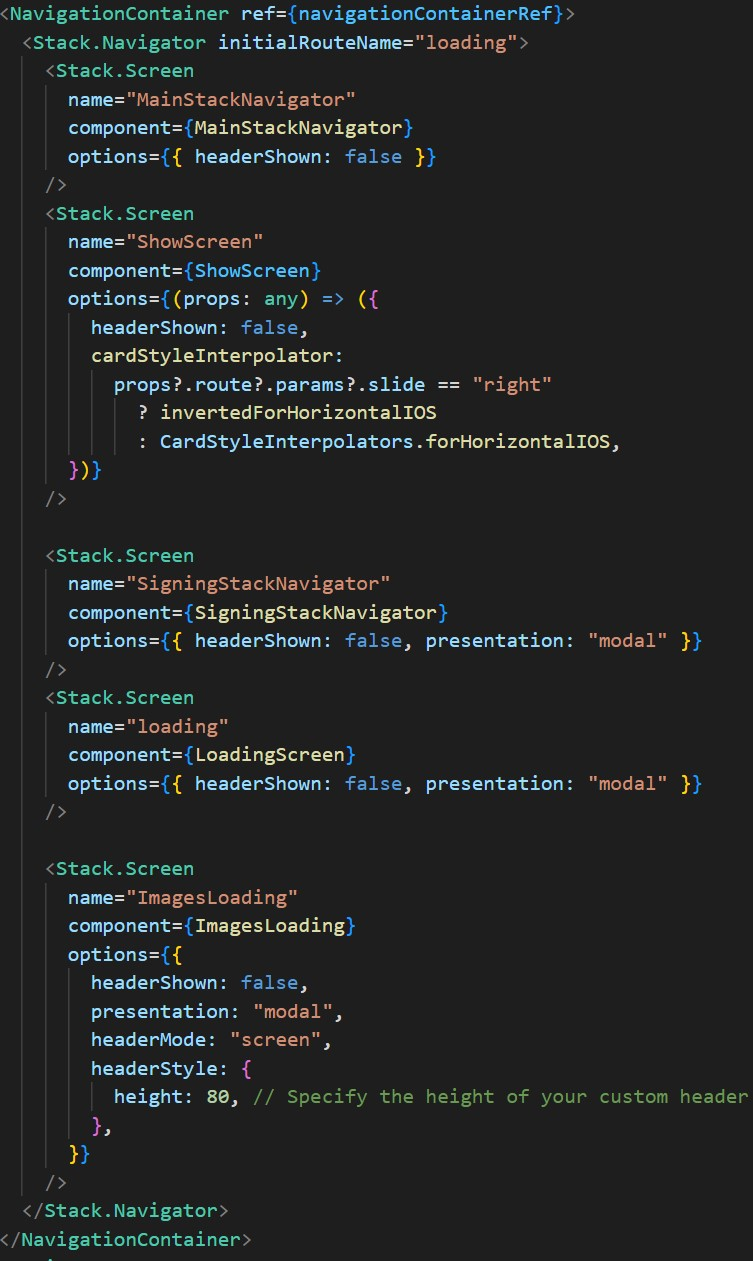
\includegraphics[width=9cm, height=15cm]{images/navigationCode.jpg}
    \caption[differenzeiteot]{Frammento di codice che gestisce la navigazione tra gli schermi}
    \label{fig:Navigation code}
\end{figure}

nella Fig 3.2, viene mostrato un frammento di codice \`e stato preso dal file App.tsx . Come si pu\`o vedere il NavigationContainer \`e il componente in cima alla gerarchia e va ad avvolgere i vari Stack Navigator:
\begin{enumerate}
    \item Il primo \`e quello immediatamente successivo al NavigationContainer e viene utilizzato per gestire la transizione verso:
          \begin{list}{*}{}
              \item Gli altri due Stack Navigator
              \item Lo schermo di loading iniziale
              \item Lo schermo per la visualizzazione delle immagini memorizzate in cache
              \item Lo screen che mostra i dettagli di un'immagine
          \end{list}
    \item Il Secondo si chiama MainStackNavigator e gestisce la navigazione tra l'index Screen e il Seach Screen.
    \item Il terzo si chiama SigningStackNavigator e gestisce la navigazione tra lo screen di sign in e quello di sign up.
\end{enumerate}

\section{Stati all'Interno dell'Applicazione}
All'interno dell'applicazione vi sono diversi stati che vengono continuamente aggiornati; per tenere traccia di ognuno di essi sono stati utlizzati le librerie \textit{redux} e \textit{react-redux}.
Attraverso di esse si va a creare uno \textit{store} che contiene l'intero stato dell'applicazione come un semplice oggetto JavaScript.

Per poter modificare gli stati vengono utilizzate delle funzioni pure chiamate
\textit{reducers} che specificano come cambia lo stato in risposta ad una \textit{action}. I \textit{reducers} prendono come argomento un'azione con un payload e restituiscono un nuovo stato basato sull'azione passata. Essendo funzioni pure non modificano i dati
dell'oggetto che viene passato e non eseguono alcun effetto collaterale nell'applicazione; dato lo stesso stesso oggetto dovrebbero produrre sempre lo stesso risultato.
Le \textit{action} devono avere una propriet\`a ``type" per indicare il tipo di azione da eseguire. Esse rappresentano l'unica fonte di informazioni per lo \textit{store} \cite{ReduxSite}.
%Le \textit{action} passate ad ogni reducer sono degli oggetti JavaScript inviati attraverso il metodo nativo di React, chiamato dispatch(). 

\begin{figure}[h]
    \begin{minipage}[b]{0.47\textwidth}
        \centering
        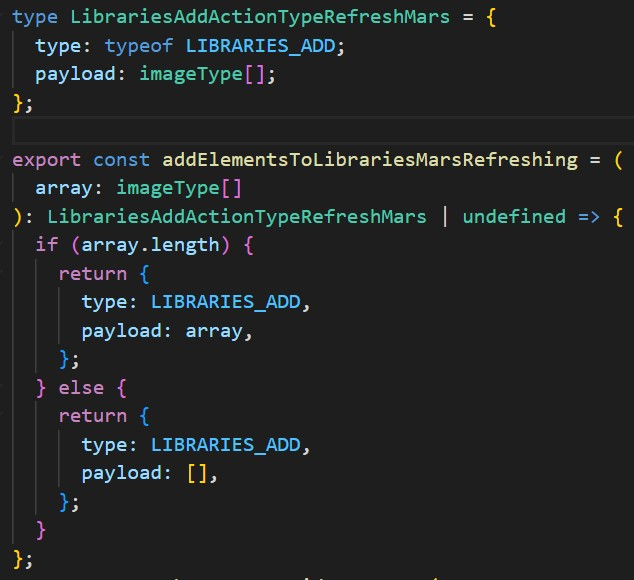
\includegraphics[width=6cm, height=6cm]{images/ActionRedux.jpg}
        \caption{\label{f_etichetta1} Esempio di \textit{action}}
    \end{minipage}
    \hfill
    \begin{minipage}[b]{0.47\textwidth}
        \centering
        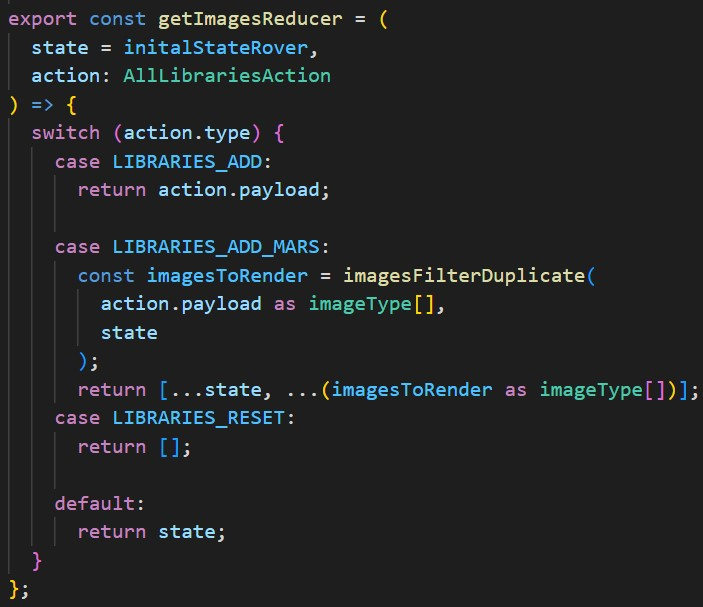
\includegraphics[width=6cm, height=6cm]{images/ReduxReducersFunction.jpg}
        \caption{\label{f_etichetta2}Esempio di \textit{reducer}}
    \end{minipage}
\end{figure}

Sia le \textit{action} che i \textit{reducer} vengono definiti come delle arrow function. La \textit{action} rappresentata nella Fig 3.3 viene utilizzata per indicare che l'array contenente le immagini che devono essere visualizzate a schermo, deve essere aggiornato.
Un \textit{action} ritorna sempre un oggetto che contiene due propriet\`a ovvero type e payload: La prima viene utilizzata per indicare al \textit{reducer} quale azione deve essere eseguita, mentre la seconda rappresenta il contenuto con cui deve essere aggiornato lo stato all'interno dello store.

Il \textit{reducer} rappresentato nella Fig 3.4, riceve sempre due parametri, che sono state e action: il primo rappresenta lo stato memorizzato nello store e viene sempre passato da quest'ultimo ogni volta che il \textit{reducer} viene invocato; l'\textit{action} rappresenta l'azione che il \textit{reducer} deve eseguire.
In base all'azione passata si entrer in uno dei diversi ``case" dello switch.

Supponendo che venga eseguita l'\textit{action} mostrata nella Fig 3.3, si entrerebbe nel primo ``case" dello switch e si andrebbe a sostituire lo stato attuale con il payload fornito dall'\textit{action}.

Le \textit{action} passate ad ogni reducer sono degli oggetti JavaScript inviati attraverso il metodo nativo di React, chiamato dispatch() che prende come parametro la \textit{action} stessa. Per poter invocare questo metodo
\`e necessario utilizzare un hook, chiamato ``useDispatch".

Oltre a poter memorizzare gli stati all'interno dello store \`e anche possibile accedere ai dati contenuti in essi attraverso un altro hook, chiamato ``useSelector".
Gli state memorizzati nello store sono:
\begin{enumerate}
    \item dataRover: un oggetto JavaScript che contiene le informazioni riguardanti la ricerca fatta dall'utente.
    \item images: un array che contiene tutte le immagini che, una volta filtrate, devono essere visualizzate a schermo.
    \item imagesHide: un array che contiene tutte le immagini che sono state occultate dall'utente.
    \item loading: \`e una variabile booleana che indica quando deve essere presentata all'utente un'animazione.
    \item search: \`e una variabile booleana che permette di avviare una procedura di ricerca.
    \item sign: viene utilizzato per memorizzare il JWT che \`e stato fornito all'utente in fase di registrazione o login.
\end{enumerate}
\begin{figure}[h]
    \centering
    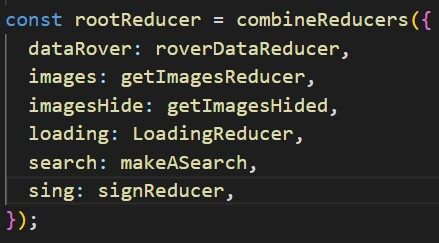
\includegraphics[width=9cm, height=5cm]{images/state.jpg}
    \caption[differenzeiteot]{A sinistra lo state memorizzato nello store e a destra il rispettivo reducer}
    \label{fig:state}
\end{figure}
\section{Fetching delle Immagini}
Ogni volta che l'utente effettua una nuova ricerca digitando il nome di un Rover oppure la data solare in cui sono state scattate le immagini, viene effettuata una richiesta HTTP ai server della Nasa; in particolare, viene effettuata una GET request \cite{Axios}.

Per effettuare richieste HTTP \`e stato utilizzato Axios, un Client HTTP che ritorna una \textit{Promise}, la quale rappresenta l'eventuale completamento {}(o fallimento) di un'operazione asincrona e il suo conseguente valore \cite{Promise}.
\begin{figure}[h]
    \centering\`a
    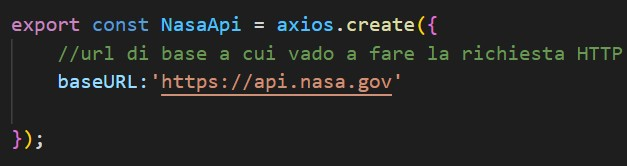
\includegraphics[width=6cm, height=2cm]{images/baseUrl.jpg}
    \caption[differenzeiteot]{Base URL}
    \label{fig:baseUrl}
\end{figure}
\begin{figure}[h]
    \centering
    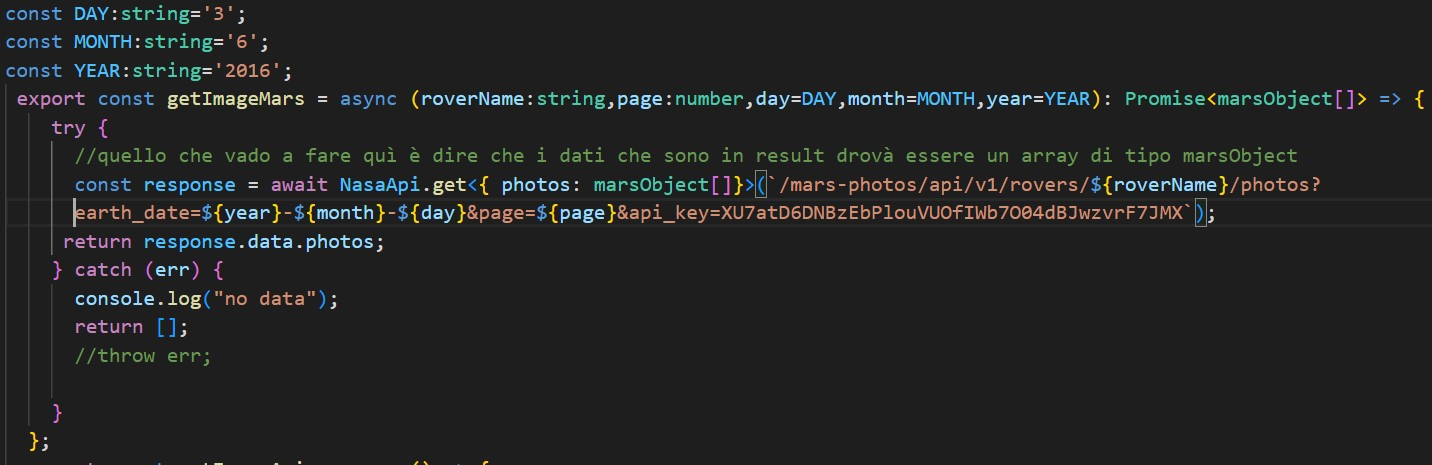
\includegraphics[width=14cm, height=5cm]{images/getRequest.jpg}
    \caption[differenzeiteot]{Esempio di richiesta GET}
    \label{fig:getRequest}
\end{figure}

Per poter eseguire una GET request finalizzata al recupero delle immagini, come nella Fig 3.7, \`e necessario fornire al metodo ``get" dell'Axios instance {}(creata nella Fig 3.6) L'URL a cui deve deve essere effettuata la richiesta e i parametri per ricercare le immagini; in particolare questi ultimi sono:
\begin{list}{*}{}
    \item Il nome del Rover {}(required)
    \item La data solare in cui sono state scattate le foto {}(required)
    \item Il numero di pagina a cui si vuole accedere {}(optional)
\end{list}
Si evidenzia che la data solare viene impostata ad un valore iniziale in modo da poter presentare all'utente un certo tipo di immagini nel momento in cui apre l'applicazione per la prima volta.

Il metodo GET utilizzato ritorna una ``Axios Response", la quale \`e un oggetto che contiene diverse propriet\`a tra cui ``data". Attraverso essa \`e possibile accedere alla risposta fornita dai server della Nasa in formato JSON.

\section{Presentazione delle Immagini}
Per visualizzare le immagini che sono state recuperate dai server della Nasa, viene utilizzato un Core Component chiamato FlatList, reso disponibile da React Native.
Questo componente presenta diverse \textit{prop}, in particolare nel mio Applicativo sono state usate le seguenti \cite{FlatList}:
\begin{itemize}
    \item data: a questa \textit{prop} deve sempre essere passata un array; in questo caso l'array di immagini che devono essere visualizzate a schermo.
    \item renderItem: a questa \textit{prop} deve essere passata una funzione o un function component che verr\`a eseguito per ogni elemento dell'array che \`e stato fornito alla prop data.
          Nel caso di questa applicazione a renderItem viene passato un ``Function Component" chiamato \textit{PhotoComponent} il quale permette di visualizzare ognin immagine e il suo id.
    \item keyExtractor: questa \textit{prop} viene utilizzata per estrarre una chiave univoca per ogni elemento della lista. In questo modo \`e possibile riodinare gli elementi se alcuni di essi venissero
          eliminati o ne venissero aggiunti altri. In questo applicativo ad ogni elemento della lista viene associato come chiave univoca l'id di ogni immagine.
    \item listFooterComponent: questa \textit{prop} permette di visualizzare un React Element/Component alla fine della lista; in questo applcativo le viene passato un React Element chiamato \textit{FooterComponent} che permette di visualizzare due link: Privacy and Policy e Log Out.
    \item onEndReached: a questa \textit{prop} viene passata una funzione invocata ogni volta che viene raggiunta la fine della lista.
          In questo applicativo, una volta raggiunta l'ultima immagine recuperata dalla ricerca precedente, viene effettuata una nuova richiesta ai server della Nasa, utilizzando gli stessi parametri di ricerca, recuperando la pagina di immagini successiva. Quest'ultima potrebbe o meno contenere delle immagini: nel caso
          in cui ve ne siano, verranno inserite in coda all'array visualizzate a schermo; in caso contrario le immagini visibili all'utente rimarranno le stesse.
\end{itemize}

\begin{figure}[h]
    \centering
    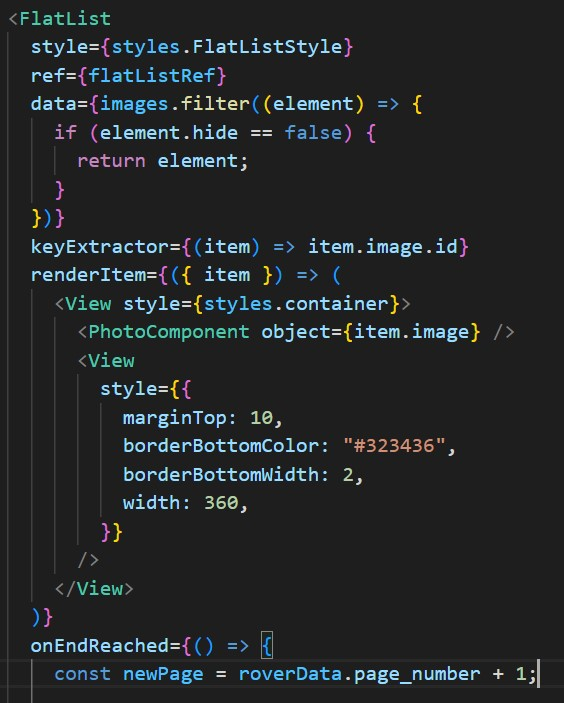
\includegraphics[width=7cm, height=10cm]{images/FlatListPrimaParte.jpg}
    \label{fig:FlatListPrimaParte}
\end{figure}

\begin{figure}[h]
    \centering
    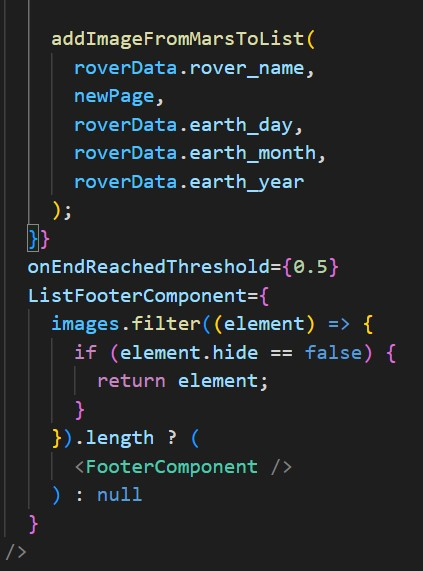
\includegraphics[width=7cm, height=10cm]{images/FlatListSecondaParte.jpg}
    \caption[differenzeiteot]{Esempio di uso della Flat List}
    \label{fig:FlatListSecondaParte}
\end{figure}

Ogni volta che l'utente chiude l'applicazione e poi la riapre, gli vengono subito mostrate delle immagini secondo dei parametri di ricerca predefiniti. Per andare a recuperare queste immagini
viene utilizzato un hook di React chiamato useEffect, al quale vengono assegnate due dipendenze: Search e allButtonColor. La prima dipendenza \`e uno state
che viene aggiornato ogni volta che un utente vuole effettuare una nuova ricerca di immagini; il secondo \`e uno state che viene aggiornato ogni volta che l'utente preme sul
pulsante ``all", esprimendo in questo modo l'intenzione di voler eseguire una ricerca.

Lo useEffect mostato nella Fig 3.9 non viene eseguito solo quando l'utente apre l'applicazione per la prima volta, ma anche ogni volta che effettua una nuova ricerca di immagini.
Tutte le volte che viene eseguito il frammento di codice nella Fig 3.9 viene aggiornato lo state \textit{dataRover}, andando a modificare il numero di pagina da recuperare. Inoltre viene invocata una funzione chiamata ReplaceImageFromMarsList{}(),
la quale va a recuperare le nuove immagini da mostrare all'utente.
\begin{figure}[h]
    \centering
    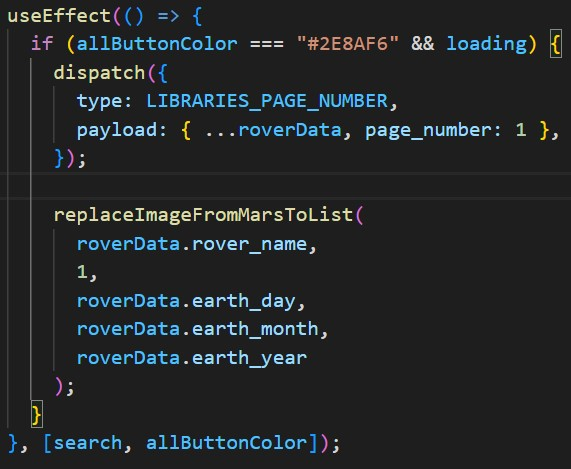
\includegraphics[width=7cm, height=7cm]{images/useEffect.jpg}
    \caption[differenzeiteot]{UseEffect per il caricamento delle immagini}
    \label{fig:useEffect}
\end{figure}
\subsection*{ReplaceImageFromMarsList()}
Come si pu\`o vedere nella Fig 3.10, questa funzione richiede che le vengono passati alcuni parametri:
\begin{itemize}
    \item Il nome del Rover per cui deve essere eseguita la ricerca.
    \item La pagina che contentiene le immagini da recuperare: questa funzione viene eseguita ogni volta che l'utente vuole ricercare nuove immagini, quindi sar\`a necessario recuperare sempre la prima pagina.
    \item Gli ultimi tre parametri corrispondono al giorno, mese e anno terrestre in cui sono state scattate le foto.
\end{itemize}

Questa funzione va ad invocare un metodo, chiamato getImageMars(), il quale va ad eseguire una GET request per recuperare le nuove immagini; una volta ottenute, si controlla che l'utente abbia premuto il tasto ``Photos" e quindi voglia visualizzare o meno le immagini nascoste.
Nel primo caso si va ad aggiornare lo state ``images" con tutte le foto recuperate; nel secondo caso viene aggiornato lo state "images" solo con le immagini che l'utente non ha occultato in precedenza.

Potrebbe accadere che l'utente fornisca dei parametri di ricerca errati e in tal caso verr\`a mostrato un messaggio di errore.

Le immagini recuperate vengono mostrate a schermo solo dopo che lo state ``loading" verr\`a posto a ``false": questo avviene dopo quattro secondi tramite l'utilizzo di una funzione asincrona, chiamata setTimeout.
\begin{figure}[h]
    \centering
    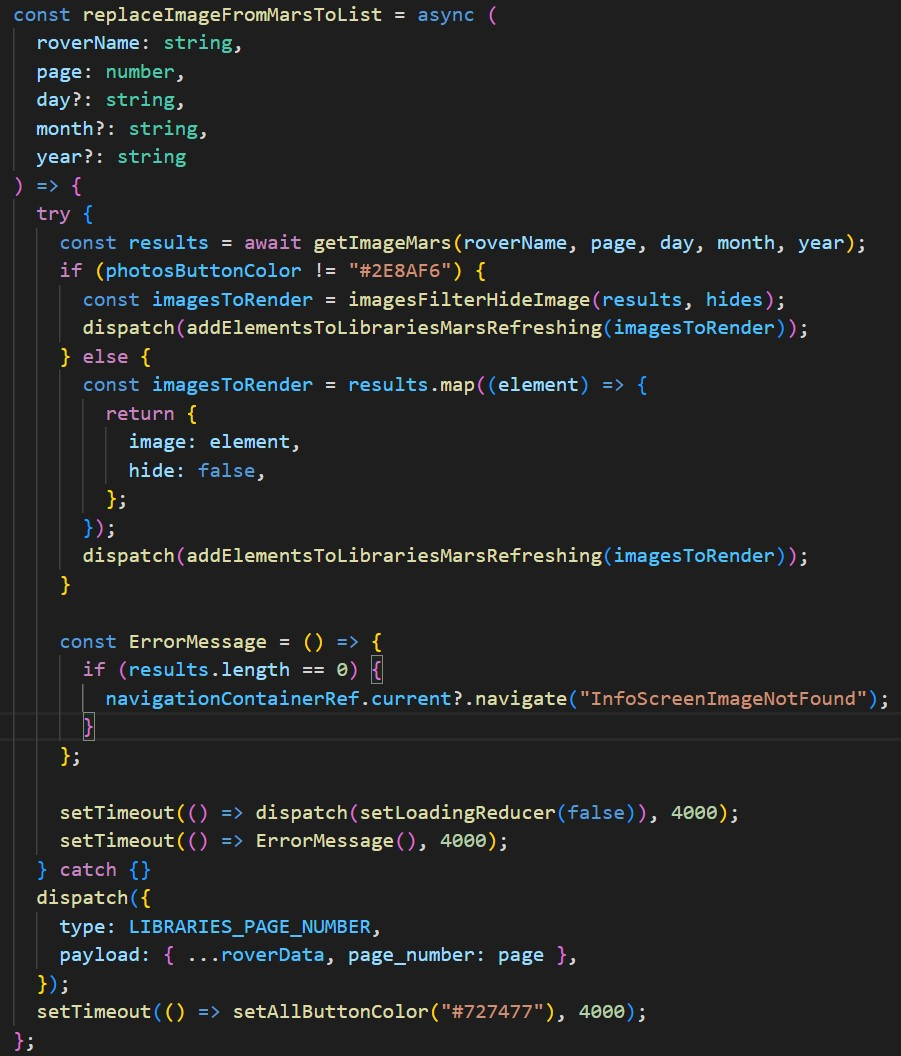
\includegraphics[width=10cm, height=14cm]{images/ReplaceImageFunction.jpg}
    \caption[differenzeiteot]{Funzione replaceImageFromMarsList}
    \label{fig:replaceImageFunction}
\end{figure}

\section{Ricerca Immagini per Nome Rover e per Data Solare}
Per poter ricercare delle immagini tramite il nome del Rover, viene fornita una search-bar il cui componente corrsipendente \`e mostrato nella fi 3.11. Quando l'utente abilita la ricerca premendo sul pulsante ``All" e poi digita nella Search-bar il nome di uno dei Rover, vengono emesse tre azioni:
\begin{itemize}
    \item Viene modificato lo state che mantiene le informazioni sui parametri di ricerca forniti dall'utente, aggiornando quindi il campo RoverName.
    \item Viene posto a true lo state ``loading", in modo da mostrare un'animazione che informi l'utente dell'avvio della ricerca.
    \item Viene modificato lo state ``search", in modo che venga eseguito lo useEffect mostrato in Fig 3.9.
\end{itemize}
\begin{figure}[h]
    \centering
    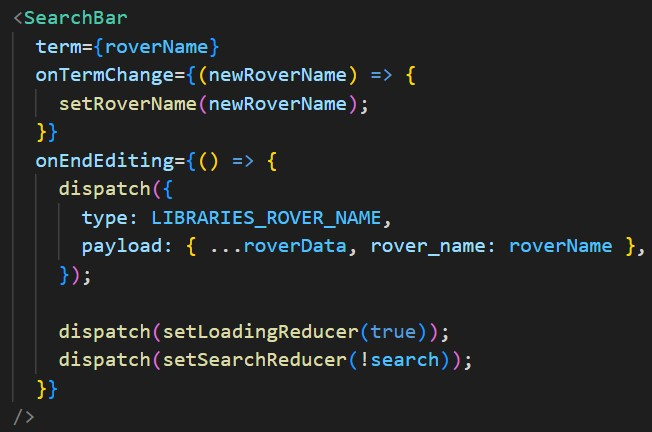
\includegraphics[width=8cm, height=6cm]{images/SearchBar.jpg}
    \caption[differenzeiteot]{Search-bar}
    \label{fig:Search-bar}
\end{figure}

Per poter ricercare delle immagini in base alla data solare vengono forniti all'utente tre campi ``input text", nei quali deve inserire giorno, mese e anno in cui sono state scattate.
Quando viene premuto il tasto ``Search by date" avviene un aggiornamento degli stati simile a quello della Fig 3.11. L'unica differenza riguarda l'aggiornamento dello stato ``dataRover": invece di
modificare il campo roverName vengono aggiornati i campi earth-day, earth-month, earth-year.

\section{Immagini Persistenti}
L'applicazione oltre a recuperare delle immagini in base ai parametri di ricerca inseriti dall'utente, deve far s\`i che vengano visualizzate solo le foto che non occultate in precedenza. Inoltre, le ultime immagini visualizzate dall'utente, devono essere presentate a quest'ultimo quando andr\`a a riaprire l'applicazione.
Per soddisfare entrambe le richieste \`e necessario rendere gli ``state" persistenti all'interno dello store fornito da Redux: ci\`o significa che quando l'applicazione viene chiusa i dati all'interno dello store non vengano persi.

Per ottenere questo risultato \`e stata usata una libreria, chiamata \textit{react-redux}; essa richiede che venga uitlizzato un altro storage {}(AsyncStorage), che non sia quello di Redux, per memorizzare i dati che si vogliono mantenere in modo persistente.
\begin{figure}[h]
    \centering
    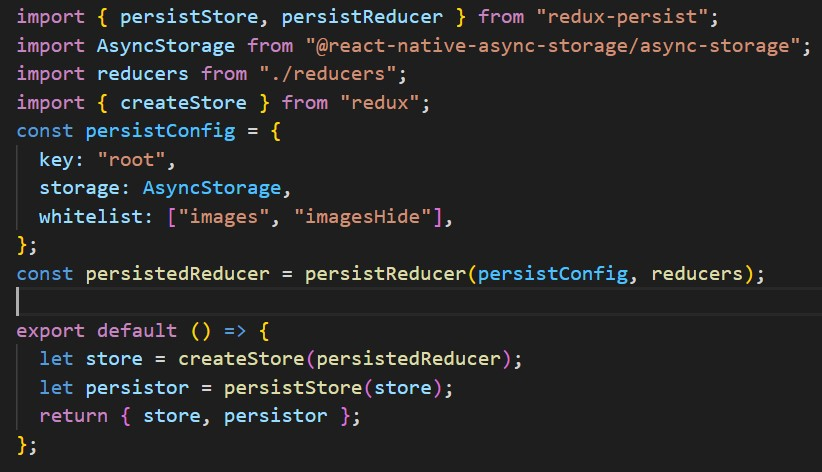
\includegraphics[width=10cm, height=7cm]{images/persistStore.jpg}
    \caption[differenzeiteot]{Creazione dello store persistente}
    \label{fig:persistStore}
\end{figure}

Come si pu\`o osservare nella Fig 3.12, react-redux richiede che vengano indicati quali stati dello store debbano essere mantenuti in modo persistente e quali no; in questo applicativo solo gli state ``images" e ``imagesHide" vengono mantenuti in questo modo.
\`E necessario poi creare lo store utilizzando la configurazione persistConfig, fornita da react-redux.

Per completare la configurazione dello store persistente si deve ``avvolgere" il NavigationContainer, che a sua volta ``avvolge" l'intera applicazione, come mostrato nella Fig 3.8.
\begin{figure}[h]
    \centering
    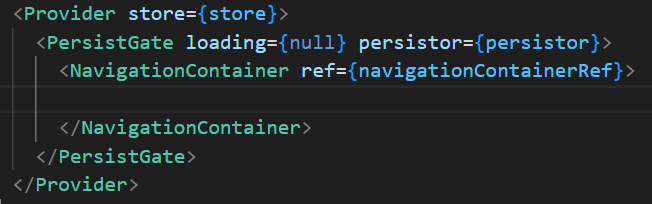
\includegraphics[width=10cm, height=4cm]{images/WrapNavigationConteiner.png}
    \caption[differenzeiteot]{Uso dello store persistente}
    \label{fig:usoStorePersistente}
\end{figure}

\section{Ripristinare le Immagini Occultate}
Una volta occultate, le immagini non vengono pi\`u visualizzate a meno che non sia l'utente a deciderlo. \`E stato realizzato un pulsante, chiamato ``Photos", che permette di ripristinare le immagini nascoste.

Nella schermata principale si hanno diversi pulsanti con uno stile simile, tra cui ``Photos": ho deciso quindi di realizzare un ``Custom component" in modo da poterlo riutilizzare per tutti i pulsanti.
Come si pu\`o osservare nella Fig 3.14, a FilterButtonComponent {}(il ``Custom component") vengono passate cinque prop: tre per configurarne lo stile e due per configurarne il funzionamento.

Ogni volta che il pulsante Photos viene premuto, il suo colore cambia da azzurro a grigio e viceversa: questo avviene grazie alla prop ``setColor".
Il cambio di colore indica una precisa azione del filtro:
\begin{itemize}
    \item Blu: vengono visualizzate anche le immagini nascoste. L'array ``images" contiene sia le foto da visualizzare che quelle nascoste, e vengono visualizzate solo quelle che possiedono la propriet\`a ``hide"= false; affinch\`e tutte le immagini vengano mostrate si deve settare la propriet\`a ``hide"
          di ogni oggetto all'interno dell'array al valore ``false". Per poter aggiornare la FlatList \`e richiesto l'aggiornamento dello stato ``images" all'interno dello store.
    \item Grigio: vengono visualizzate solo le immagini che non sono state nascoste in precedenza.
          Per ritornare alla condizione in cui solo le immagini non occultate vengono visualizzate, viene invocata la funzione dontShowImagesHide(); questa va a ripristinare l'array ``images", andando a settare correttamente la propriet\`a ``hide" di ogni oggetto all'interno di esso.
          Per poter aggiornare la FlatList \`e richiesto l'aggiornamento dello stato ``images" all'interno dello store.
\end{itemize}

\begin{figure}[h]
    \centering
    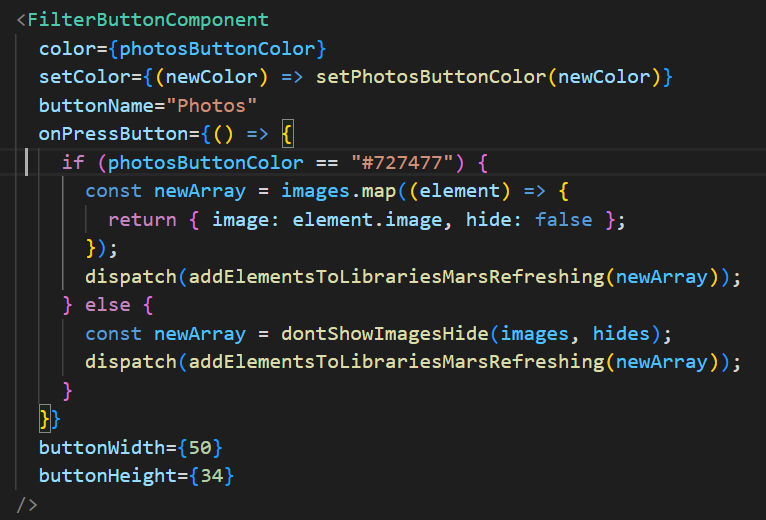
\includegraphics[width=11cm, height=8cm]{images/photoButton.png}
    \caption[differenzeiteot]{Filtro Photos}
    \label{fig:photoButton}
\end{figure}
\section{Procedura di Sign In e Sign Up}
Ogni utente prima di poter accedere all'applicazione deve disporre di un JWT (JSON Web Token); per poterlo ottenere \`e necessario fornire
e-mail e password nella schermata di login o di registrazione, a seconda che le credenziali siano gi\`a registrate nel database o meno.
Sia la procedura di \textit{sign in}  che quella di \textit{sign up} richiedono che venga contattato il server locale. In particolare, nella prima procedura viene
contattata la route localhost3000/signin, mentre nella seconda viene contattata la route localhost3000/signup.
\begin{figure}[h]
    \centering
    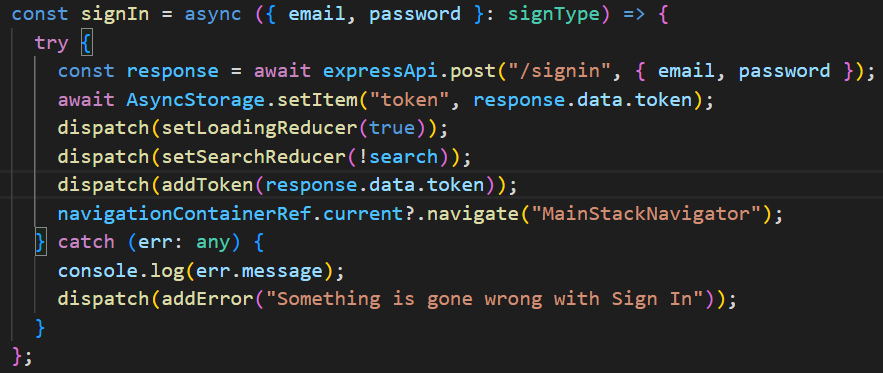
\includegraphics[width=10cm, height=5cm]{images/signInApplication.png}
    \caption[differenzeiteot]{Funzione di sign in}
    \label{fig:sign in}
\end{figure}

Come si pu\`o notare nella Fig 3.15 l'utente invia un oggetto contenente la propria e-mail e password utilizzato il metodo post della libreria Axios;
il quale invier\`a l'oggetto in formato JSON.

Se la procedura di \textit{sign in} va andare a buon fine, il server risponde con il JWT dell'utente, il quale viene salvato all'interno dell'``asyncStorage"; cos\`i facendo quando l'utente riapre
l'applicazione non deve nuovamente inserire le proprie credenziali, ma viene automaticamente loggato all'interno dell'applicazione.\\
Se invece la procedura di \textit{sign in} non va a buon fine, viene mostrato un errore all'utente in modo che capisca che le proprie credenziali non sono corrette.

La procedura di \textit{sign up} \`e identica tranne per la route che l'applicazione contatta.

Vediamo ora nel dettaglio la route di \textit{sign in} e \textit{sign up} all'interno del server.
\subsection*{Sign Up}
Come si pu\`o vedere nella Fig 3.16, la prima operazione svolta dalla route di \textit{sign up} consiste nell'andare ad estrarre le credenziali
fornite dall'utente; una volta ottenute viene creato e poi salvato un nuovo ``user" all'interno del database tramite il metodo ``save".

Se il salvataggio avviene correttamente, si genera un JWB che viene inserito nel body della risposta inviata dal server all'applicazione.
\begin{figure}[h]
    \centering
    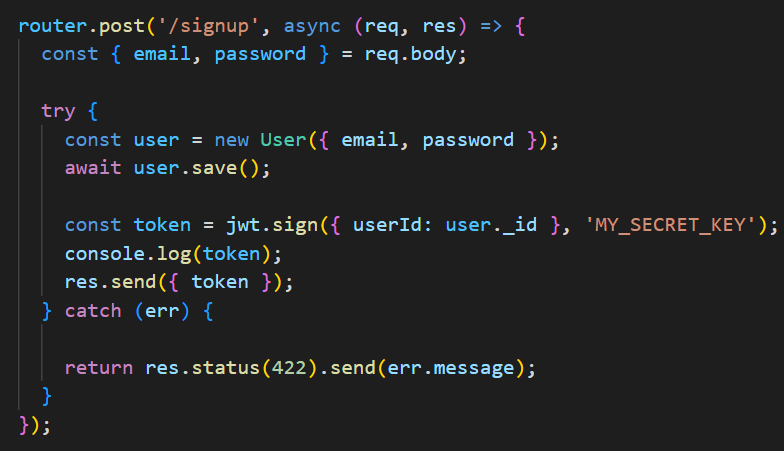
\includegraphics[width=10cm, height=6cm]{images/signUpServer.png}
    \caption[differenzeiteot]{Route di sign up}
    \label{fig:sign up}
\end{figure}

Prima di effettuare il salvataggio dell'utente nel database viene eseguita una operazione di pre-saving come mostrato nella Fig 3.17. In questa operazione viene cifrata la password fornita dall'utente.
Per eseguire la cifratura vengono usati due metodi della libreria bcrypt; ossia genSalt e hash: in particolare, il secondo permette di eseguire l'hash
della password. Quest'ultima viene poi sostituita a quella inserita dall'utente in modo che venga inserita nel database.

\begin{figure}[h]
    \centering
    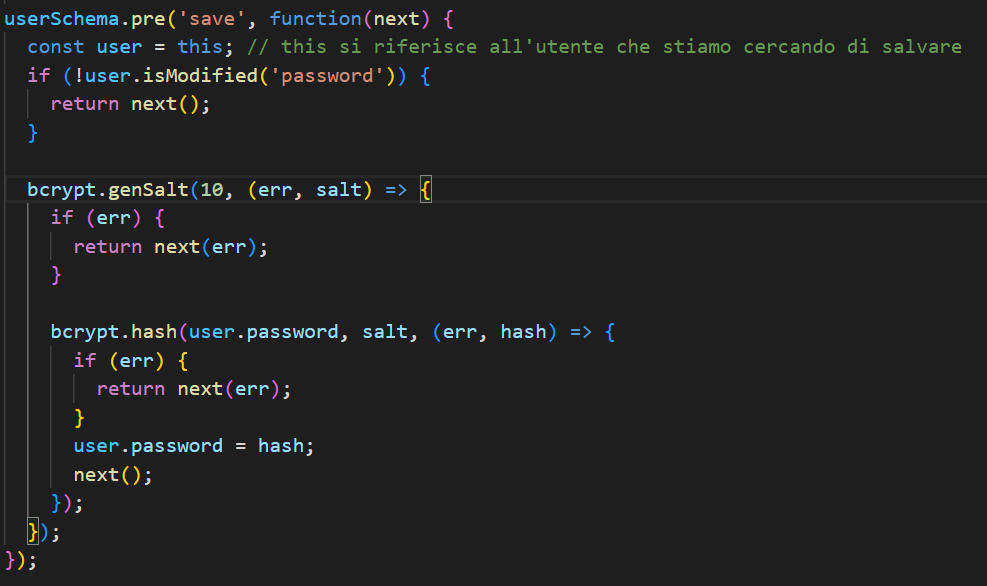
\includegraphics[width=9cm, height=6cm]{images/preSaveFunction.png}
    \caption[differenzeiteot]{Funzione di pre-saving}
    \label{fig:pre-saving}
\end{figure}


\subsection*{Sign In}

\begin{figure}[H]
    \centering
    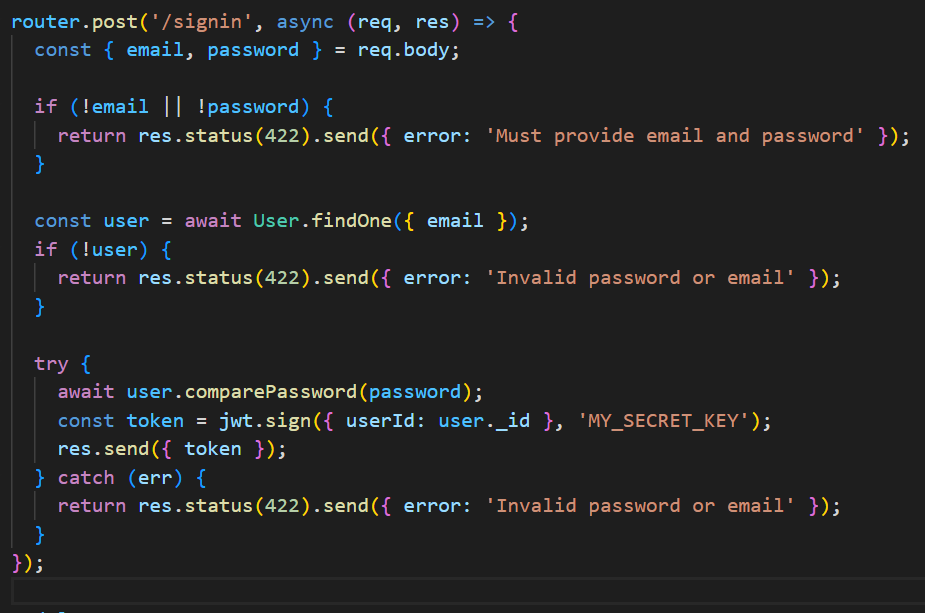
\includegraphics[width=9cm, height=6cm]{images/signinServer.png}
    \caption[differenzeiteot]{Route di sign in}
    \label{fig:Route sign in}
\end{figure}

Come si pu\`o vedere nella Fig 3.18, per prima cosa si accede alle credenziali inviate dall'utente e si controlla che siano state fornite sia un'email che una password. In seguito, attraverso l'email fornita, viene recuperata la password cifrata presente
nel database e tramite la funzione comparePassword() si confrontano le due password. Questa funzione fa uso dl metodo compare del modulo bcrypt per andare a verificare che la password fornita dall'utente e quella cifrata presente sul database siano uguali.
Se la verifica da esito positivo, viene generato un JWT tramite il metodo sign del modulo ``jsonwebtoken". il token generato viene poi inserito nel body della riposta per l'utente.


\chapter{Risultati}
In questo capitolo viene dimostrato il funzionamento dell'applicazione su un Samsung s9 e un Iphone 13, in modo da visualizzare le piccole
differenze di funzionamento e grafica sui due dispositivi.
\section{Splash Screen}
Ogni volta che l'utente apre l'applicazione viene presentato lo Splash Screen mostrato nelle Fig 4.1 e 4.2 . Osservando attentamente le due figure non si notano differenze significative, se non che la dimensione del testo nell'iPhone 13 \`e notevolmente pi\`u piccola.
Inoltre, nel dispositivo Apple il testo \`e posto pi\`u in basso nello schermo: ci\`o \`e  dovuto ad una dimensione maggiore del dispotivo fisico.

Cliccando sul pulsante ``Explore" l'utente potrebbe essere reindirizzato su due screen alternativi: ``Sign in" o ``Images Cache" .\\ \\ \\
\begin{figure}[h]
    \begin{minipage}[h]{0.47\textwidth}
        \centering
        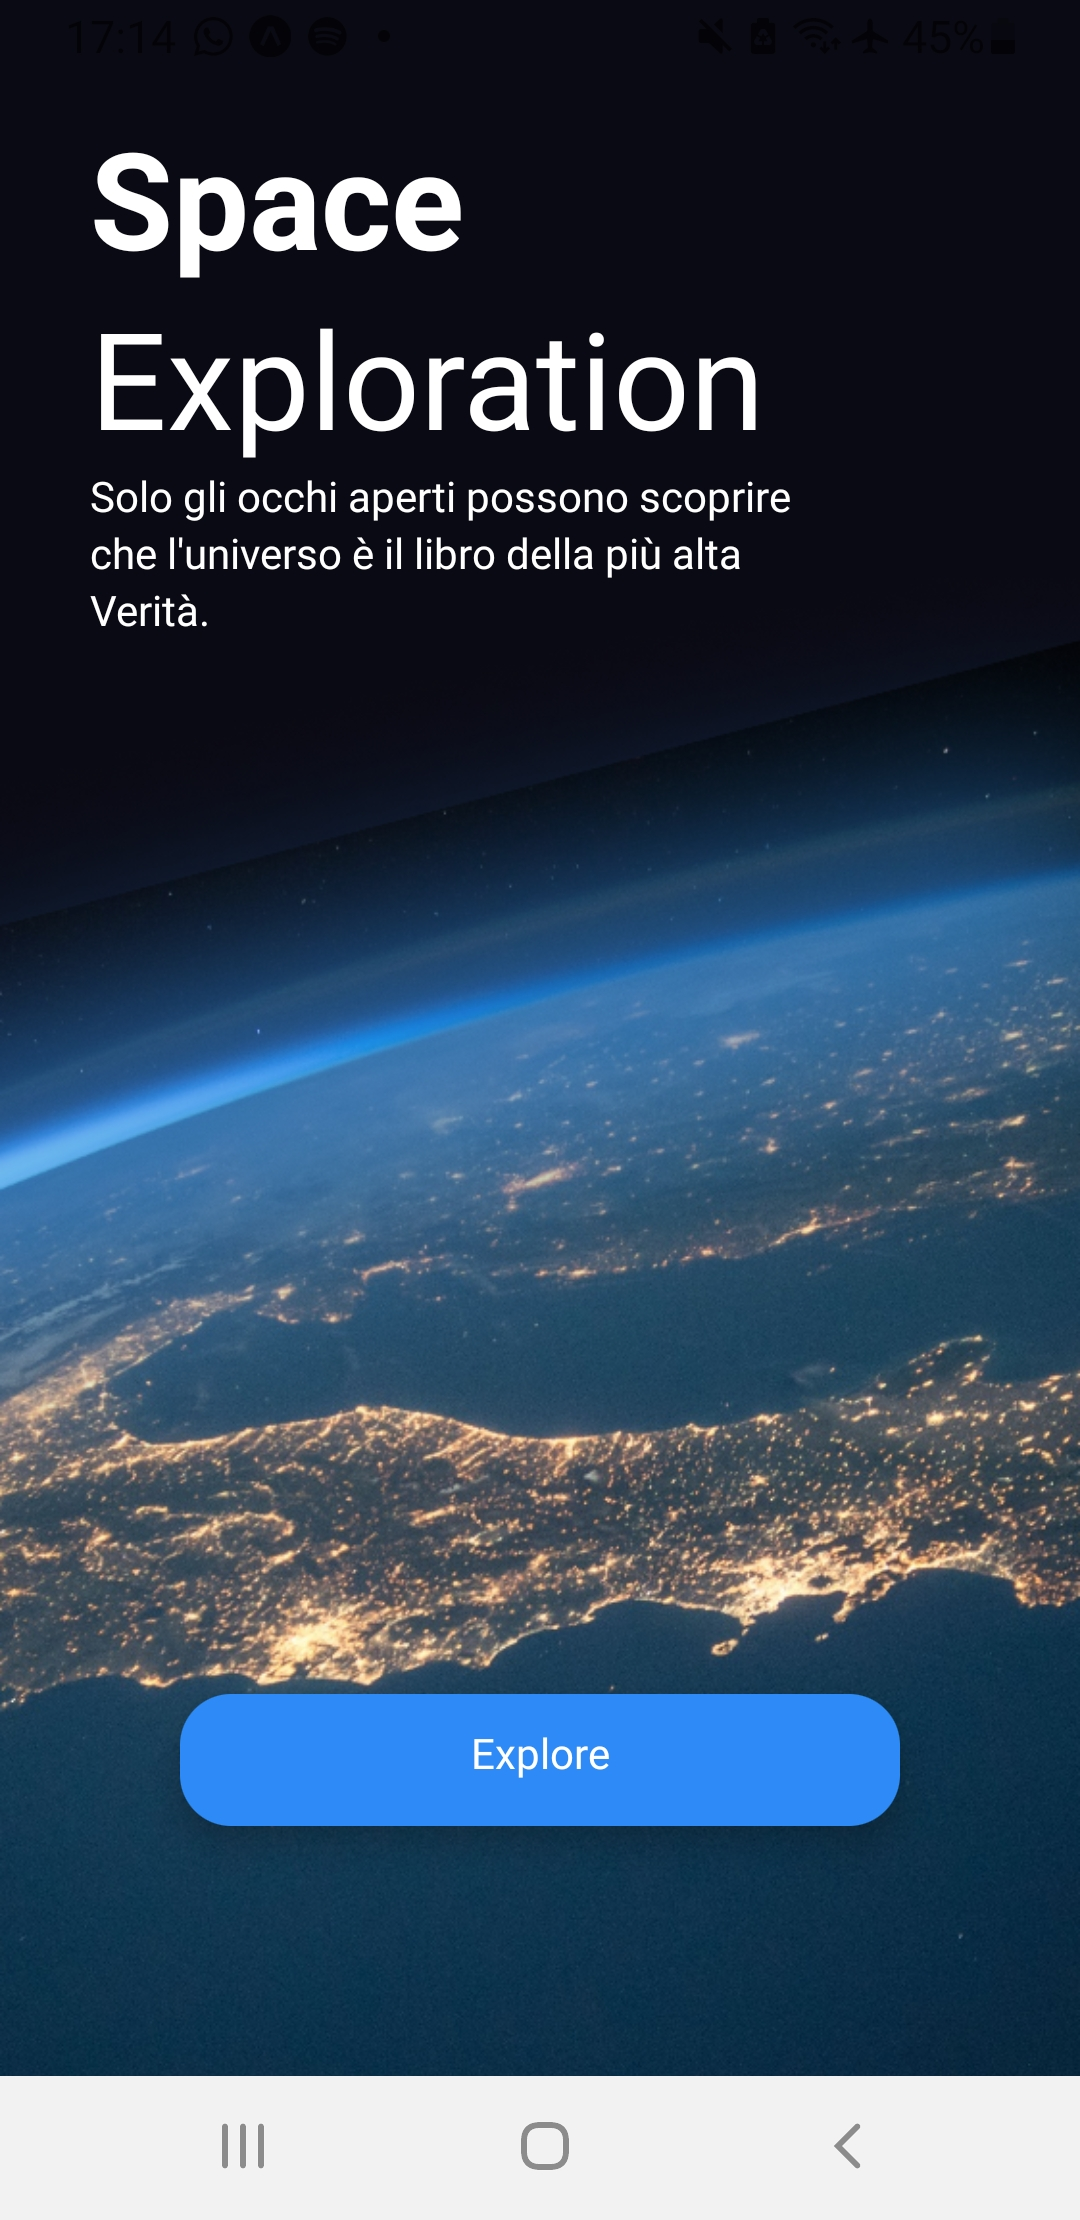
\includegraphics[width=5cm, height=10cm]{images/immaginiAndroid/splashScreen.jpg}
        \caption{\label{SpalshScreenAndroid} Android Splash Screen}
    \end{minipage}
    \hfill
    \begin{minipage}[h]{0.47\textwidth}
        \centering
        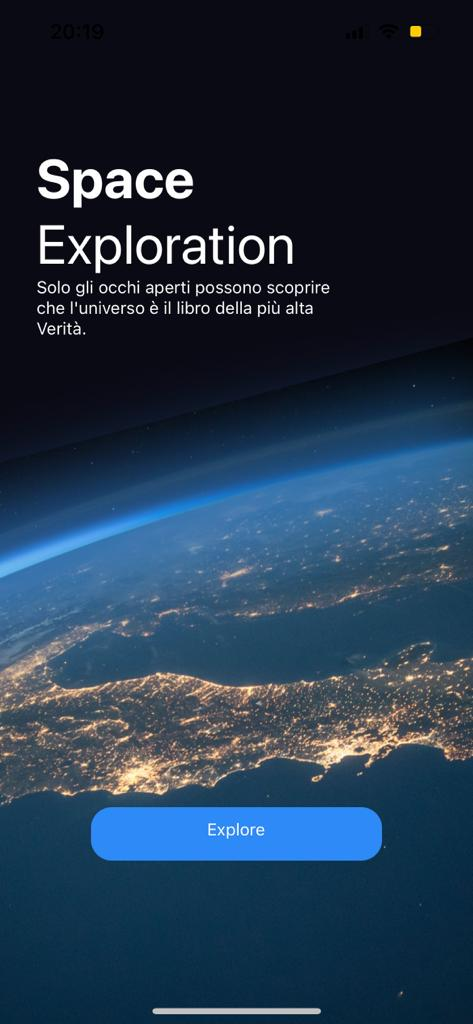
\includegraphics[width=5cm, height=10cm]{images/immaginiPhone/splashScreen.jpeg}
        \caption{\label{splashScreenIphone}iPhone Splash Screen}
    \end{minipage}
\end{figure}


\section{Sign In e Sign Up}
Se l'utente non ha mai effettuato l'accesso all'applicazione, dallo splash screen viene reindirizzato allo schermo di ``Sign in", mostrato nella Fig 4.3 (4.4 per iOS), dove pu\`o accedere al suo profilo con le proprie credenziali.
Nel caso in cui l'utente non abbia gi\`a un profilo , cliccando sul pulsante ``Sign up" viene portato nella schermata di registrazione mostrata nella Fig
4.5 (4.6 per iOS); in quest'ultima inserendo la propria e-mail e password pu\`o registrarsi ed accedere alla schermata principale.
Nel caso in cui l'utente cerchi di accedere con delle credenziali non valide oppure voglia registrarsi con una e-mail gi\`a
presente nel database, viene presentato un messaggio di errore.
\begin{figure}[H]
    \begin{minipage}[h]{0.47\textwidth}
        \centering
        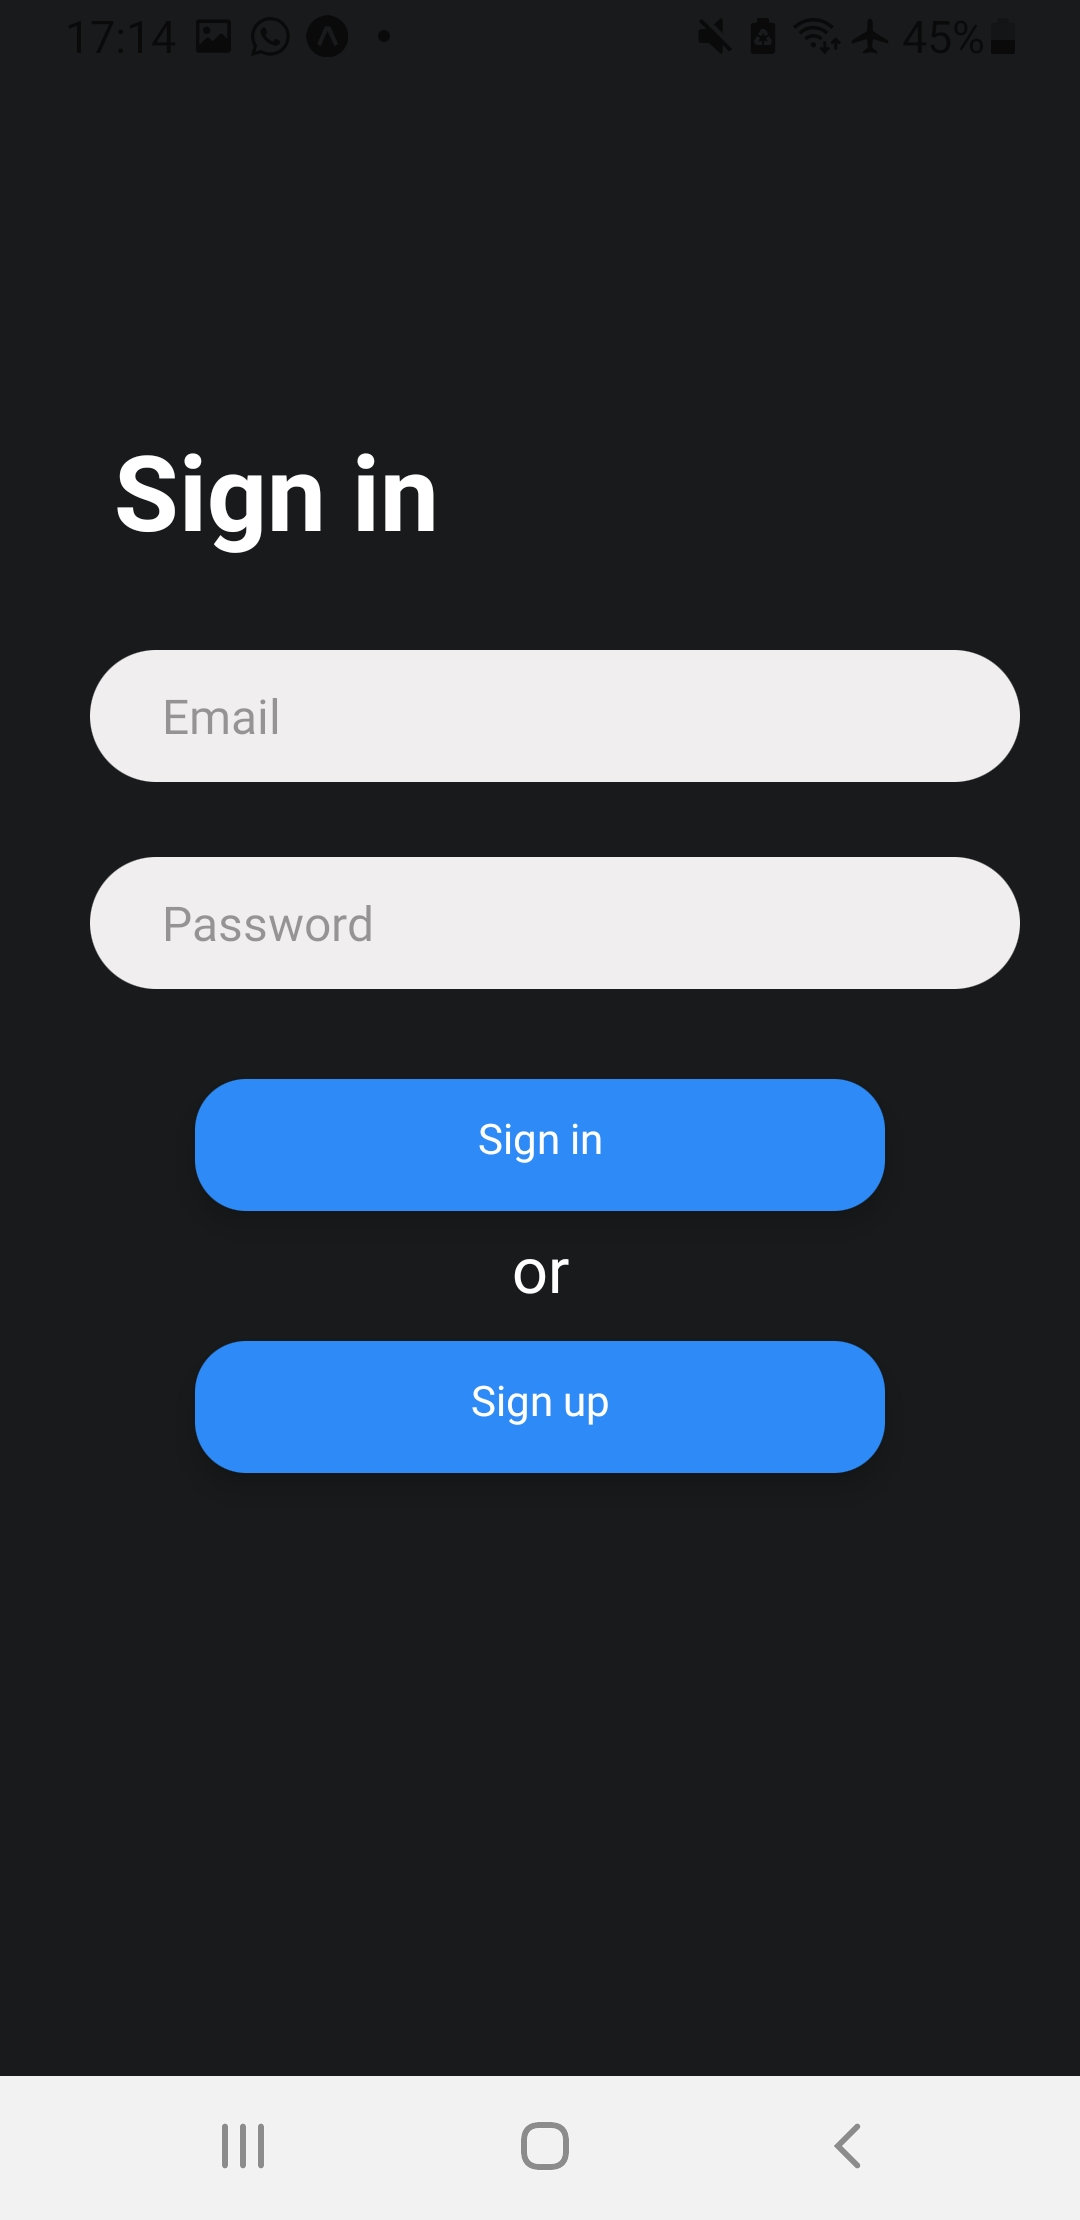
\includegraphics[width=5cm, height=10cm]{images/immaginiAndroid/signIn.jpg}
        \caption{\label{signInAndroid} Android schermo Sign In}
    \end{minipage}
    \hfill
    \begin{minipage}[h]{0.47\textwidth}
        \centering
        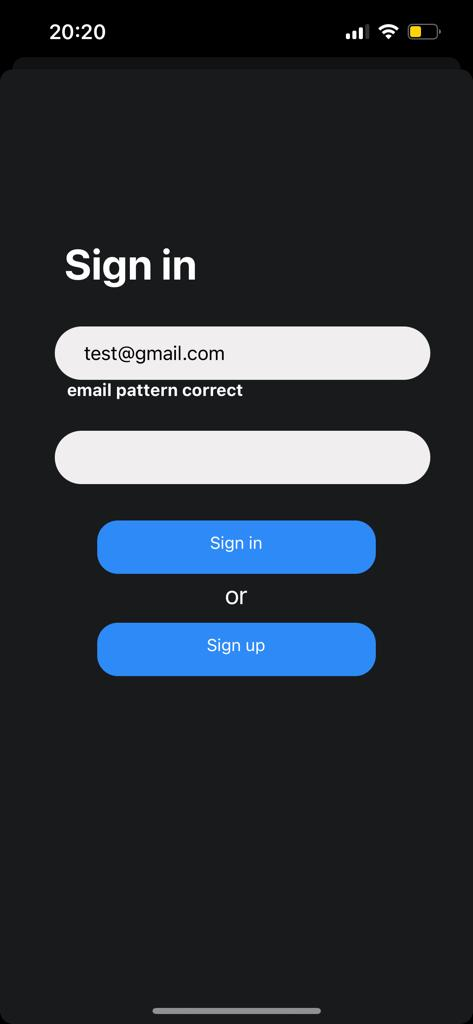
\includegraphics[width=5cm, height=10cm]{images/immaginiPhone/signIn.jpeg}
        \caption{\label{signIniPhone}iPhone schermo Sign In}
    \end{minipage}
    \begin{minipage}[h]{0.47\textwidth}
        \centering
        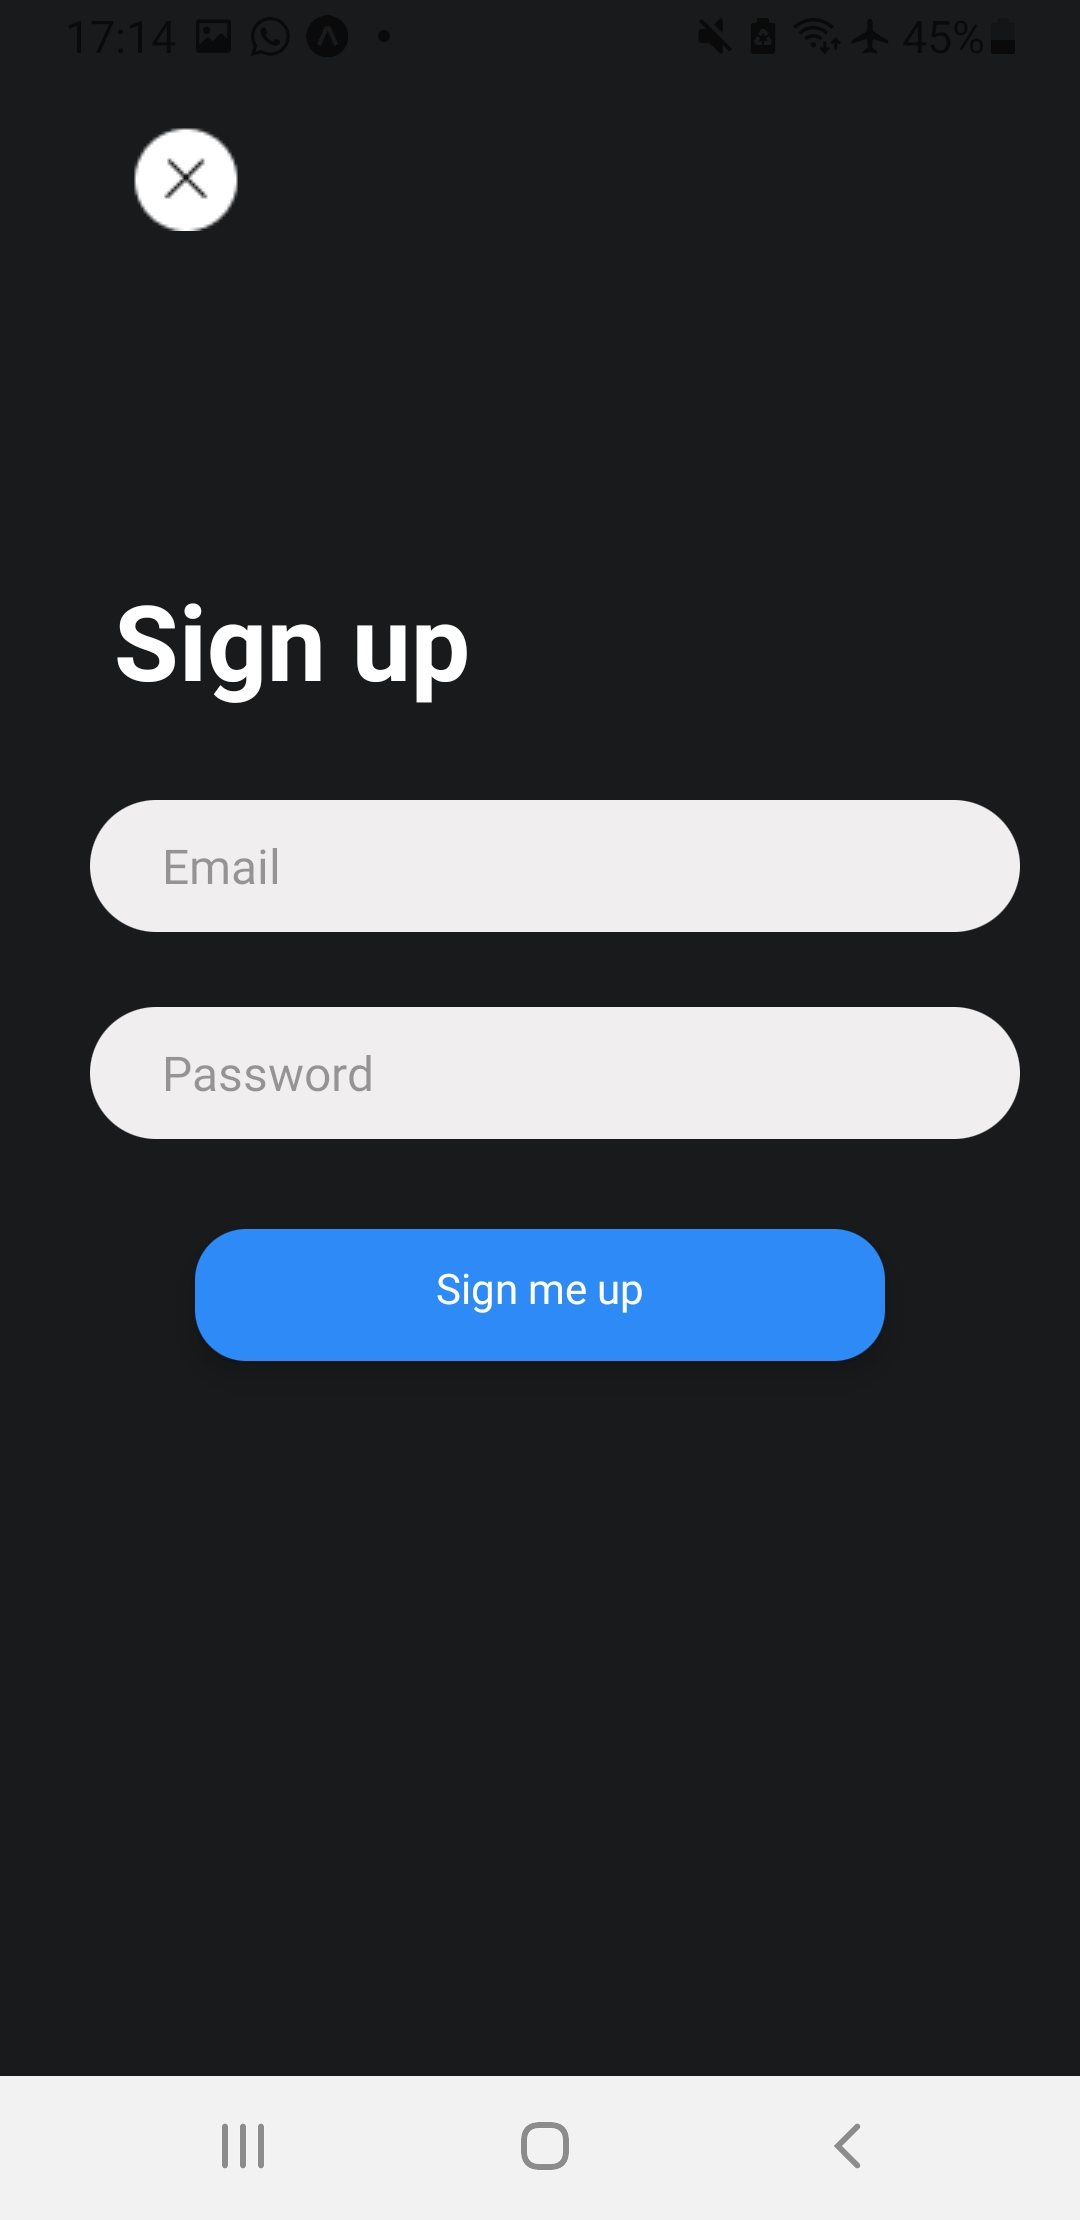
\includegraphics[width=5cm, height=10cm]{images/immaginiAndroid/signUp.jpg}
        \caption{\label{signUnAndroid} Android schermo Sign Up}
    \end{minipage}
    \hfill
    \begin{minipage}[h]{0.47\textwidth}
        \centering
        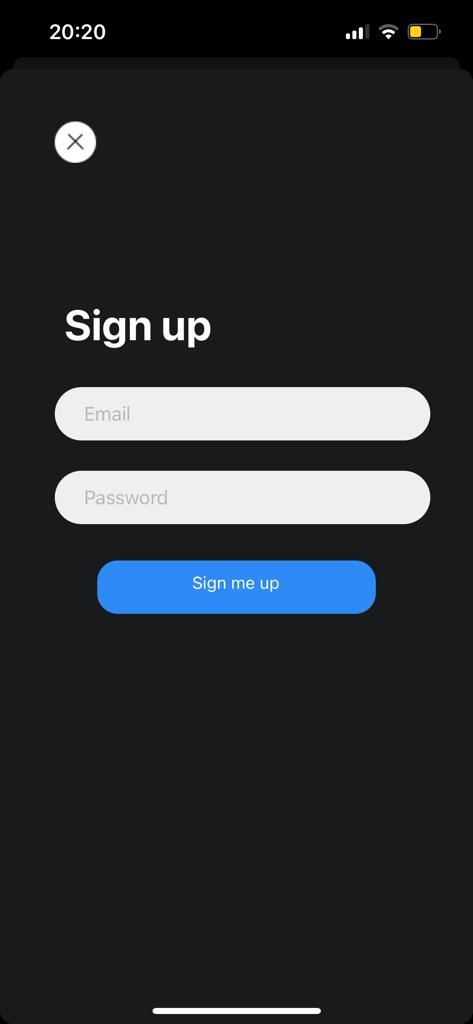
\includegraphics[width=5cm, height=10cm]{images/immaginiPhone/signUp.jpeg}
        \caption{\label{signUniPhone}iPhone schermo Sign Up}
    \end{minipage}
\end{figure}
Una volta acceduto al proprio profilo, l'utente viene reindirizzato nella schermata principale, nella quale vengono visualizzate di volta in volta le immagini ricercate.
\section{Immagini Memorizzate nella Cache}
Se l'utente ha gi\`a effettuato in precedenza l'accesso all'applicazione, nel proprio dispotivo \`e gi\`a stato memorizzato un JWT;
essendo gi\`a in possesso di questo oggetto l'utente viene reindirizzato dallo Splash Screen allo screen destinato alle immagini memorizzate nella Cache. Tale schermo \`e mostrato
nella Fig 4.7 (4.8 per iPhone) e mostra le ultime immagini che l'utente ha visualizzato prima di chiudere l'applicazione.
\begin{figure}[h]
    \begin{minipage}[h]{0.47\textwidth}
        \centering
        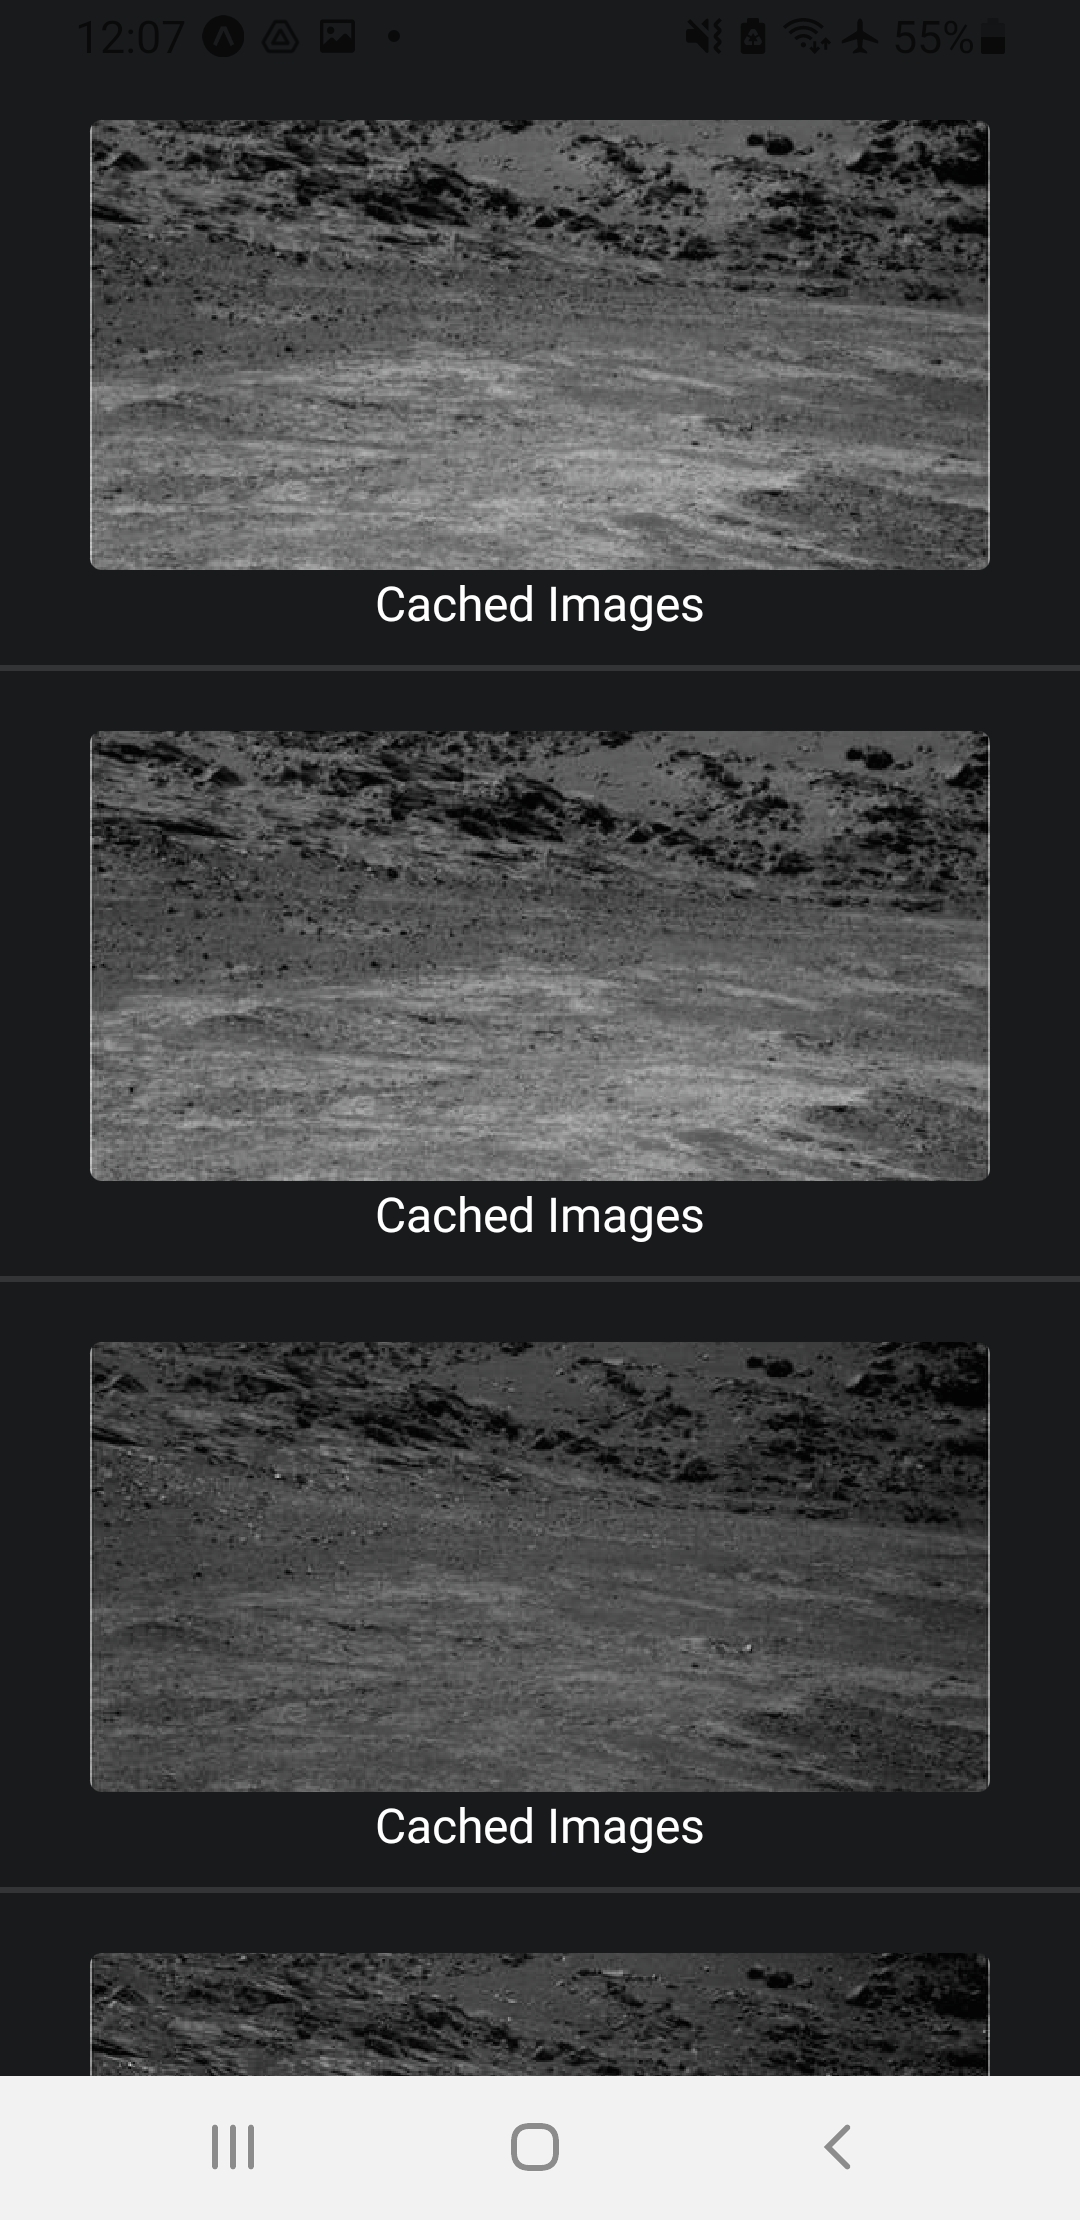
\includegraphics[width=5cm, height=10cm]{images/immaginiAndroid/imagesLoadin.jpg}
        \caption{\label{imagesLoadinAndroid} Android schermo per immagini memorizzate in cache}
    \end{minipage}
    \hfill
    \begin{minipage}[h]{0.47\textwidth}
        \centering
        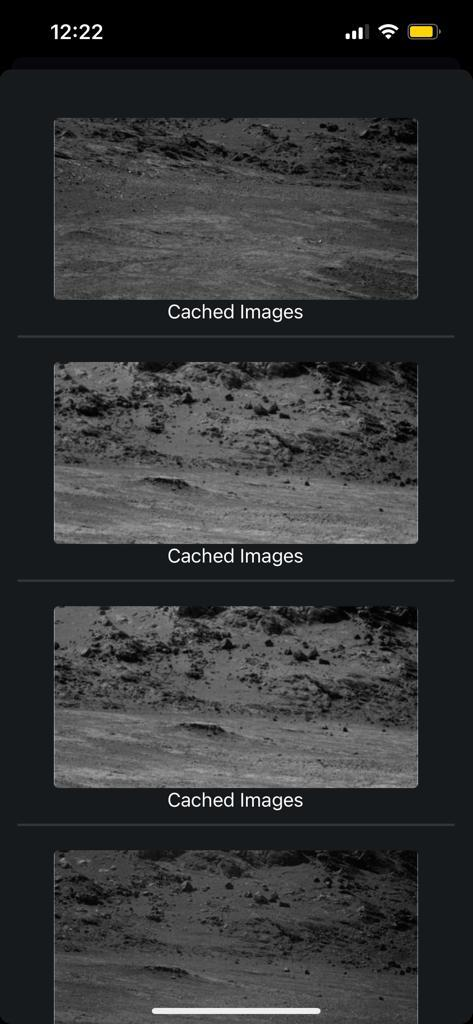
\includegraphics[width=5cm, height=10cm]{images/immaginiPhone/imagesLoading.jpeg}
        \caption{\label{imagesLoadinIphone}iPhone schermo per immagini memorizzate in cache}
    \end{minipage}
\end{figure}

Dalle Fig 4.7 e 4.8 si pu\`o evincere che l'unica differenza tra Android e iPhone \`e una maggiore distanza dall'header dello schermo.
\section{Ricerca Immagini per Nome Rover}
Per poter ricercare le immagini tramite il nome del Rover, l'utente deve:

\begin{enumerate}
    \item Assicurarsi che il pulsante ``All" non sia stato premuto, quindi sia di colore grigio.
    \item Digitare uno dei tre nomi possibili nella Search-Bar: Curiosity, Opportunity e Spirit.
    \item Cliccare sul pulsante ``All" avviando la ricerca.
\end{enumerate}

\begin{figure}[h]
    \begin{minipage}[h]{0.47\textwidth}
        \centering
        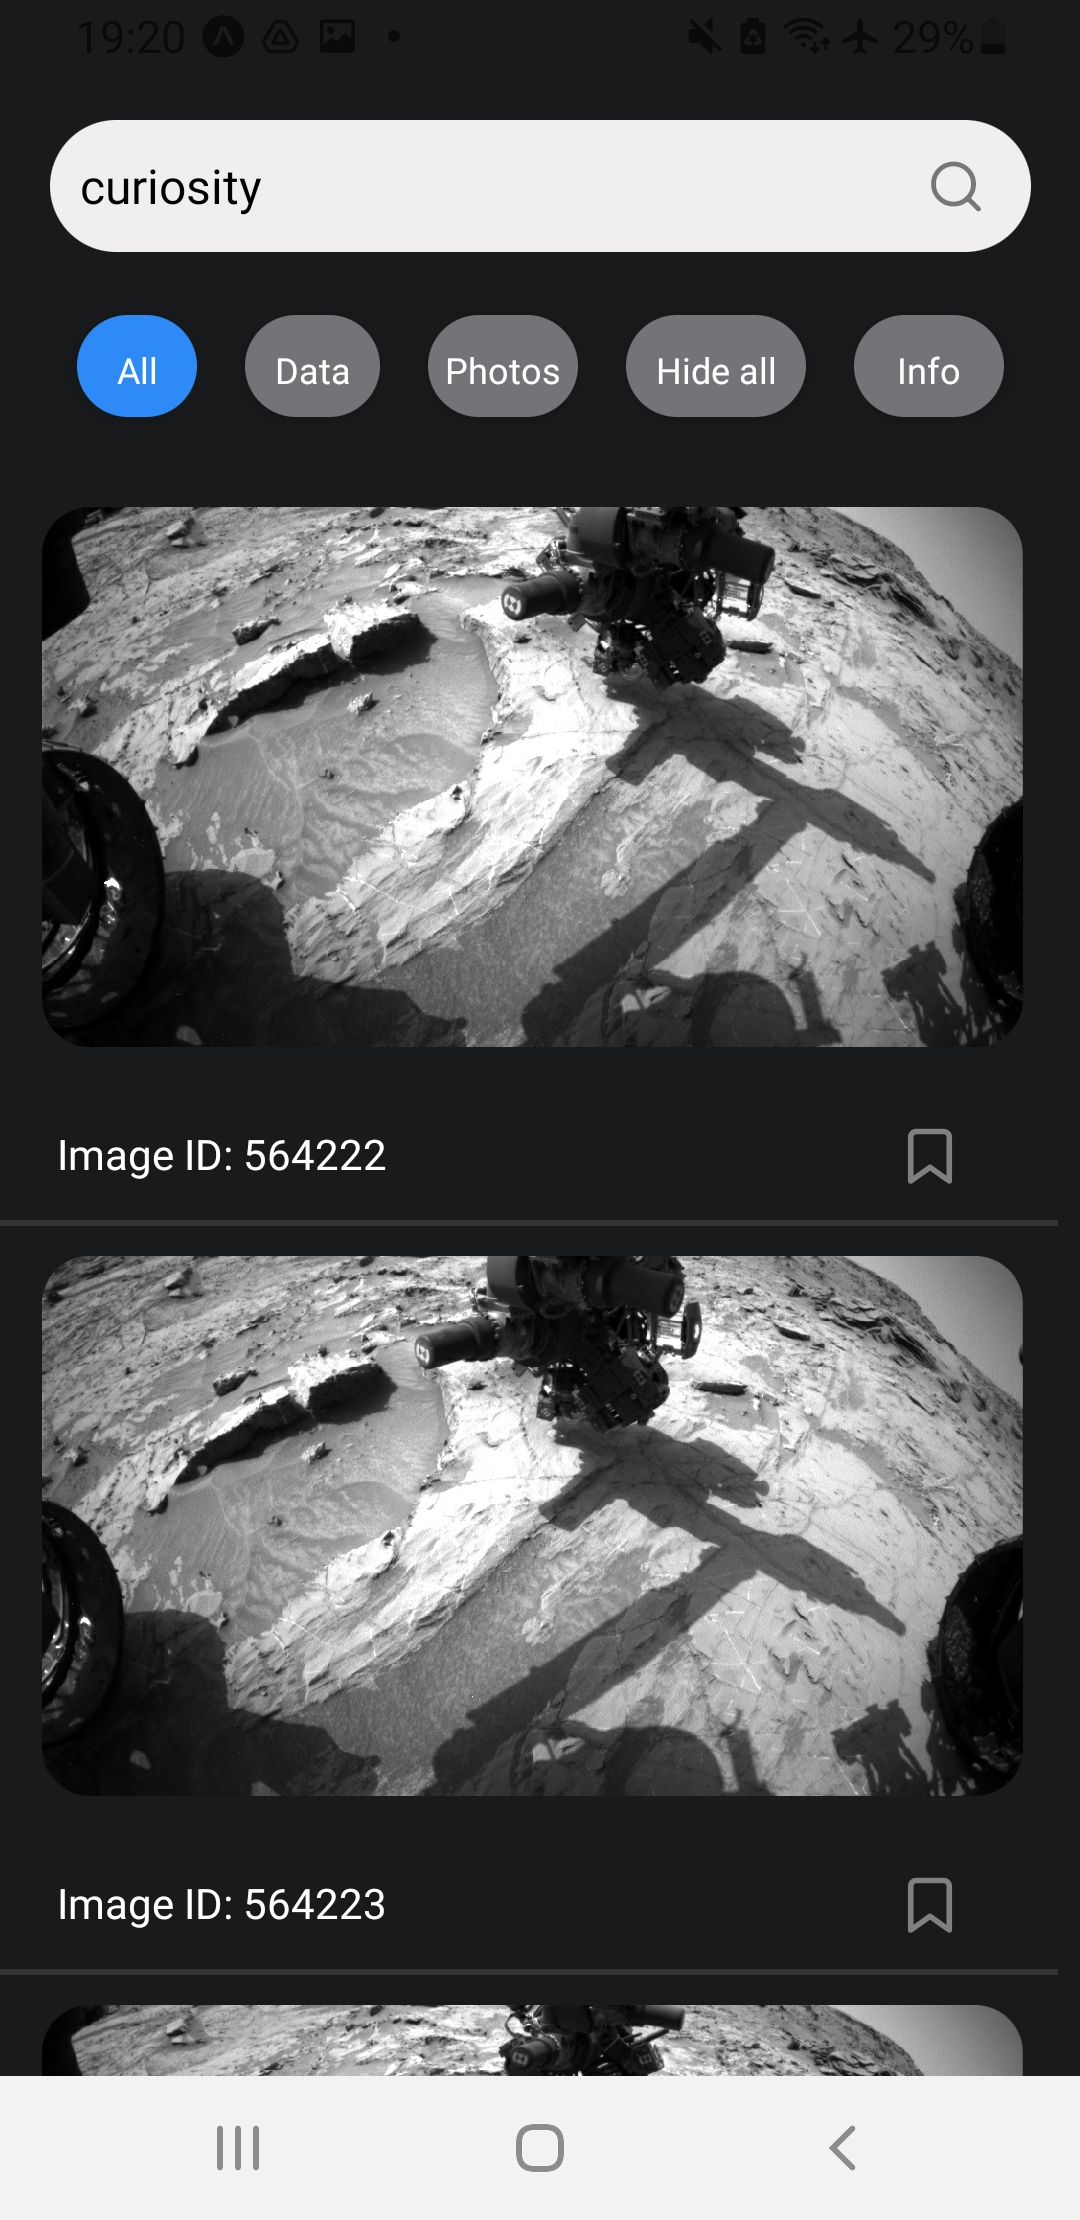
\includegraphics[width=5cm, height=10cm]{images/immaginiAndroid/ricercaNomeRover.jpg}
        \caption{\label{ricercaNomeRoverAndroid} Android ricerca per nome}
    \end{minipage}
    \hfill
    \begin{minipage}[h]{0.47\textwidth}
        \centering
        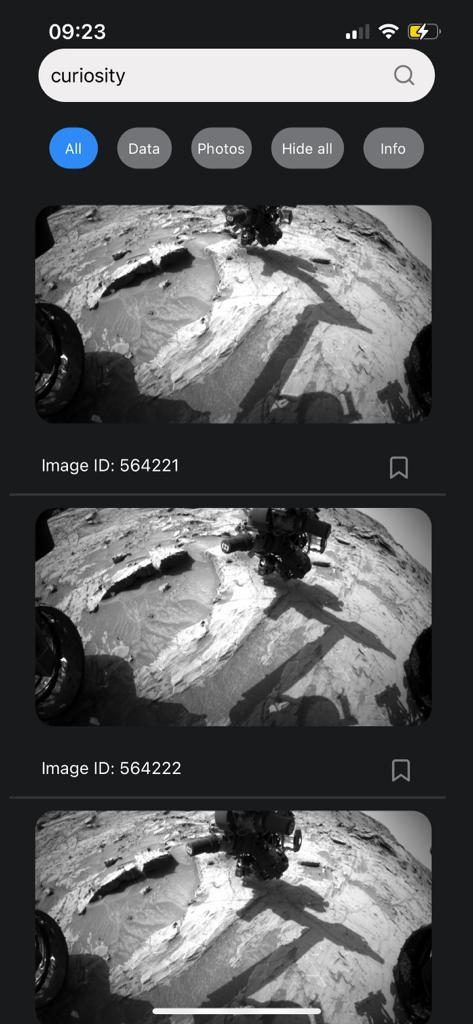
\includegraphics[width=5cm, height=10cm]{images/immaginiPhone/ricercaNomeRover.jpeg}
        \caption{\label{ricercaNomeRoverIphone}iPhone ricerca per nome}
    \end{minipage}
\end{figure}

Dalla Fig 4.9 e 4.10 non si nota nessuna differenza tra i due dispositivi: per la realizzazione di questi screen \`e stato infatti utilizzato uno stile di
presentazione chiamato ``FlexBox", il quale si adatta ai vari dispositivi su cui \`e utilizzato.

\section{Ricercare Immagini per Data Solare}
Per ricercare immagini per data solare l'utente deve premere il pulsante ``data" in modo da essere reindirizzato nello screen mostrato nella Fig 4.11 (4.12 per iPhone).
In questa schermata si possono inserire giorno, mese e anno in cui sono state scattate le immagini e premere su ``Search by date" per iniziare la ricerca.
\begin{figure}[h]
    \begin{minipage}[h]{0.47\textwidth}
        \centering
        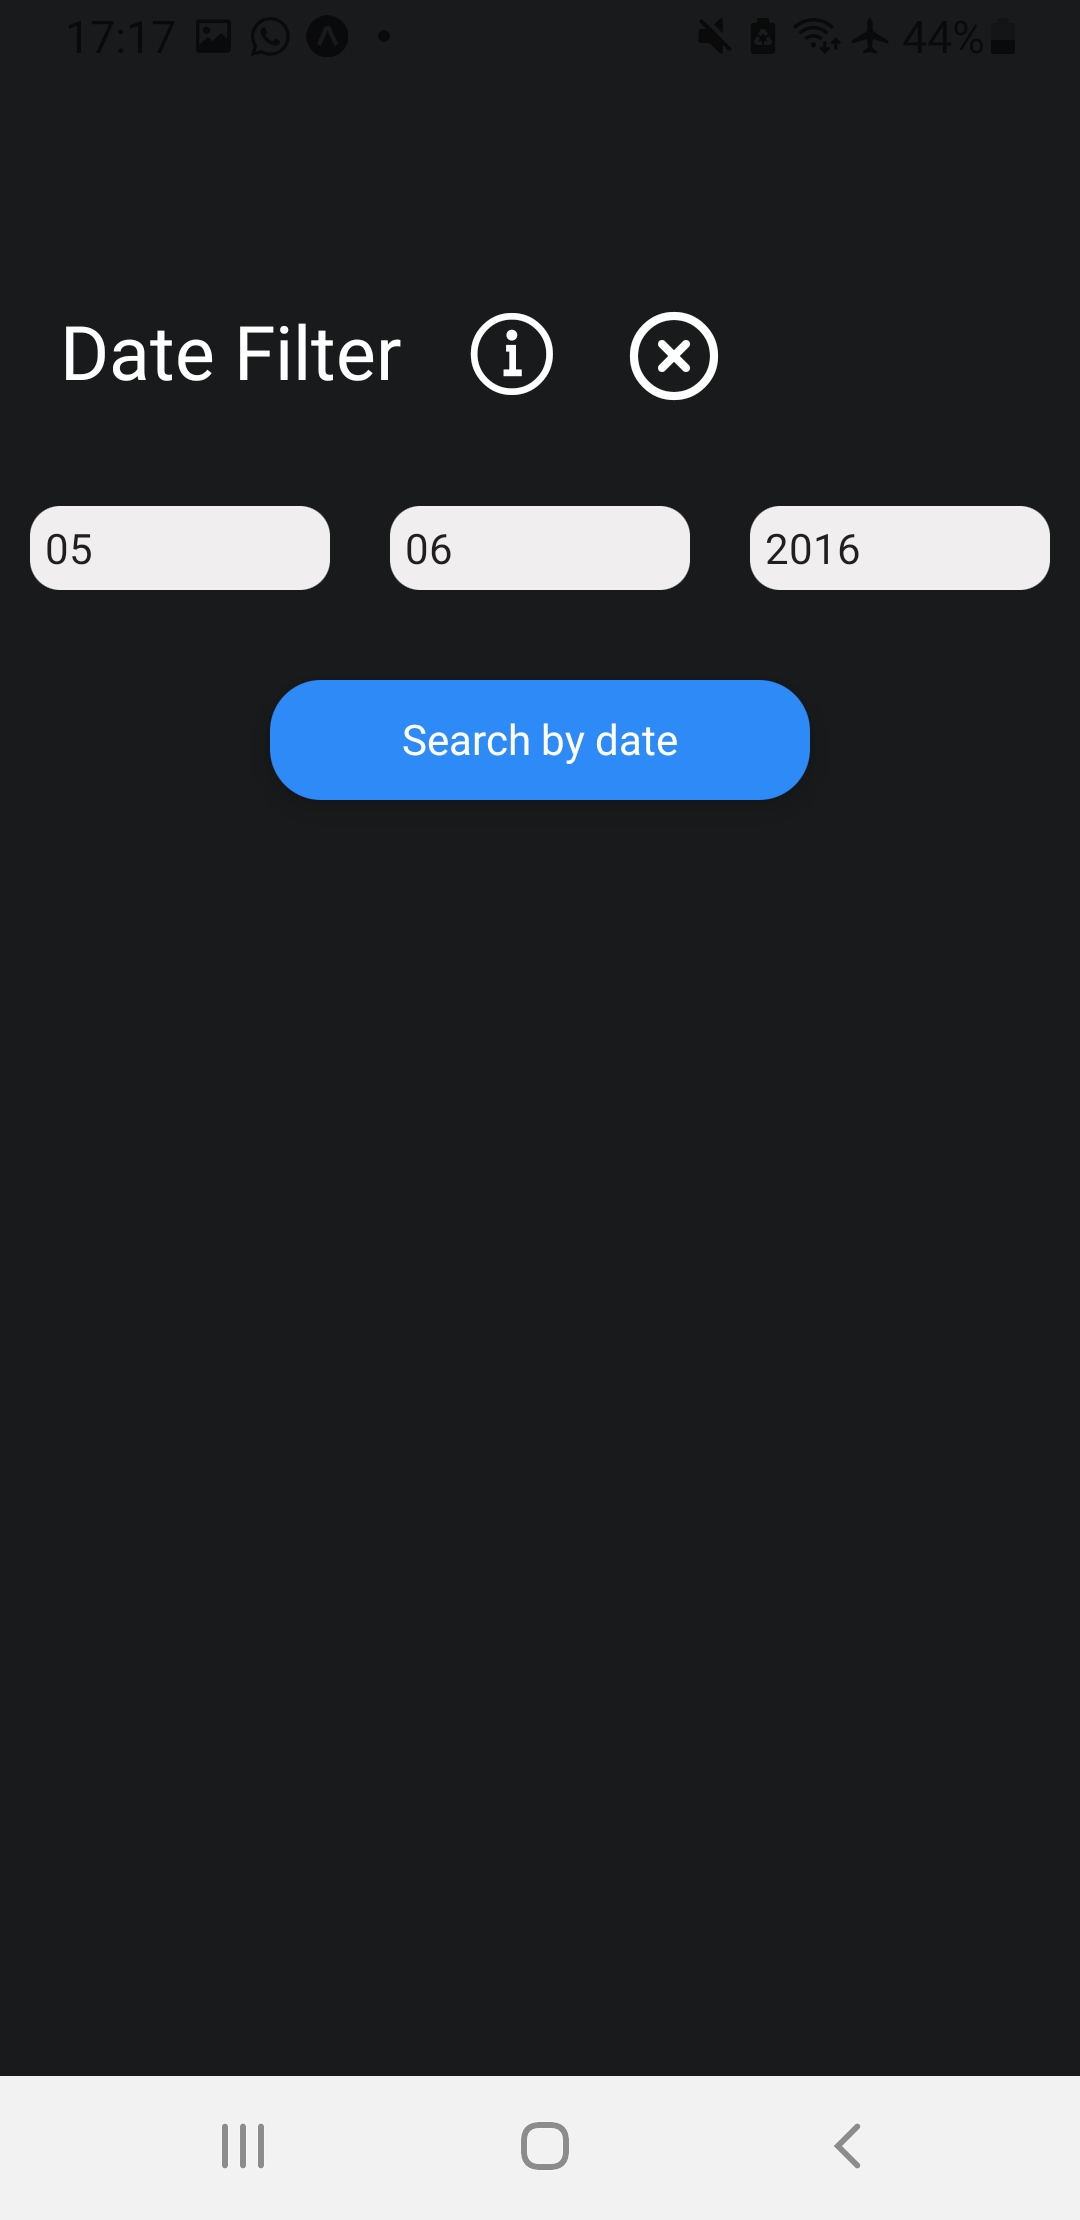
\includegraphics[width=5cm, height=10cm]{images/immaginiAndroid/SearchbyDate.jpg}
        \caption{\label{SearchbyDateAndroid} Android ricerca per data solare}
    \end{minipage}
    \hfill
    \begin{minipage}[h]{0.47\textwidth}
        \centering
        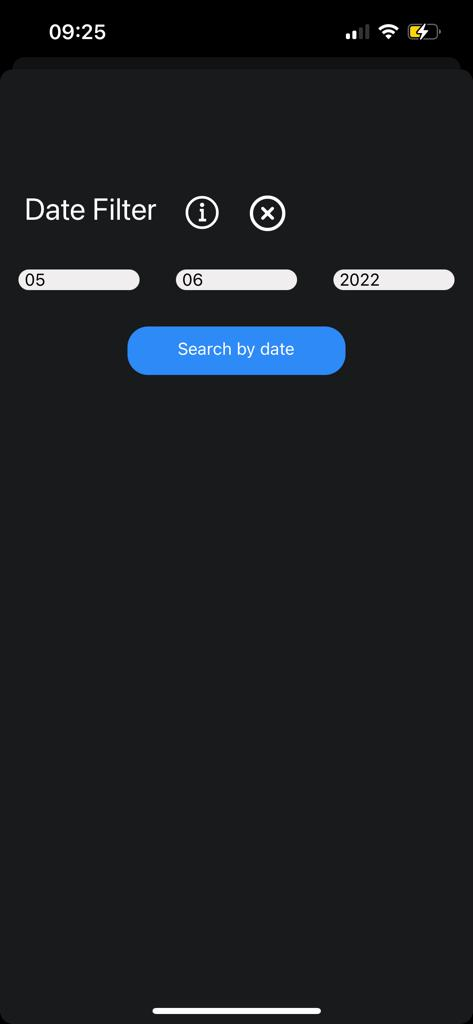
\includegraphics[width=5cm, height=10cm]{images/immaginiPhone/SearchbyDate.jpeg}
        \caption{\label{SearchbyDateIphone}iPhone ricerca per data solare}
    \end{minipage}
\end{figure}

Osservando attentamente le Fig 4.11 e 4.12 si possono notare due principali differenze tra i due dispositivi:
\begin{itemize}
    \item I campi dove l'utente pu\`o digitare il testo sono diversi, in quanto il componente TextInput di React Native viene reindirizzato in un componente nativo diverso a seconda della piattaforma di destinazione \cite{ReactNativeComponent}.
    \item Il pulsante ``Search by date" \`e diverso per lo stesso motivo descritto sopra.
\end{itemize}

\section{Dettagli delle Immagini}
Oltre a poter ricercare delle immagini \`e possibile visualizzare i dettagli di esse, come: l'ID del Rover, il nome del Rover e la camera che ha scattato la foto.
Per poter accedere ai dettagli di ogni immagine \`e necessario premere su una di esse, in modo da essere reindirizzati nello screen mostrato nella Fig 4.13 (4.14 per iOS).
In questo screen oltre a poter vedere i dettagli di una immagine \`e anche possibile nascondere la stessa premendo sul pulsante ``Hide this image".
Una volta occultata, l'immagine non viene pi\`u mostrata nella schermata principale a meno che l'utente non prema il pulsante ``Photos".

Osservando le Fig 4.13 e 4.14 possiamo notare alcune differenze tra i due dispositivi:
\begin{enumerate}
    \item Il pulsante ``Hide this image" viene presentato in modo diverso poich\`e il componente Button di React Native viene reindirizzato differentemente a seconda della piattaforma di destinazione \cite{ReactNativeComponent}.
    \item L'icona rappresentata con una ``X" si trova in due posizioni diverse sui dispositivi; in iOS \`e molto vicino all'Header dello schermo, mentre in Android si trova pi\`u in basso. Questa differenza di locazione
          \`e dovuta al fatto che l'icona \`e stata posizionata utilizzando come dimensione i pixel dello schermo e quindi non \`e responsive rispetto alle dimensioni di ogni dispotivo.
\end{enumerate}

\begin{figure}[h]
    \begin{minipage}[h]{0.47\textwidth}
        \centering
        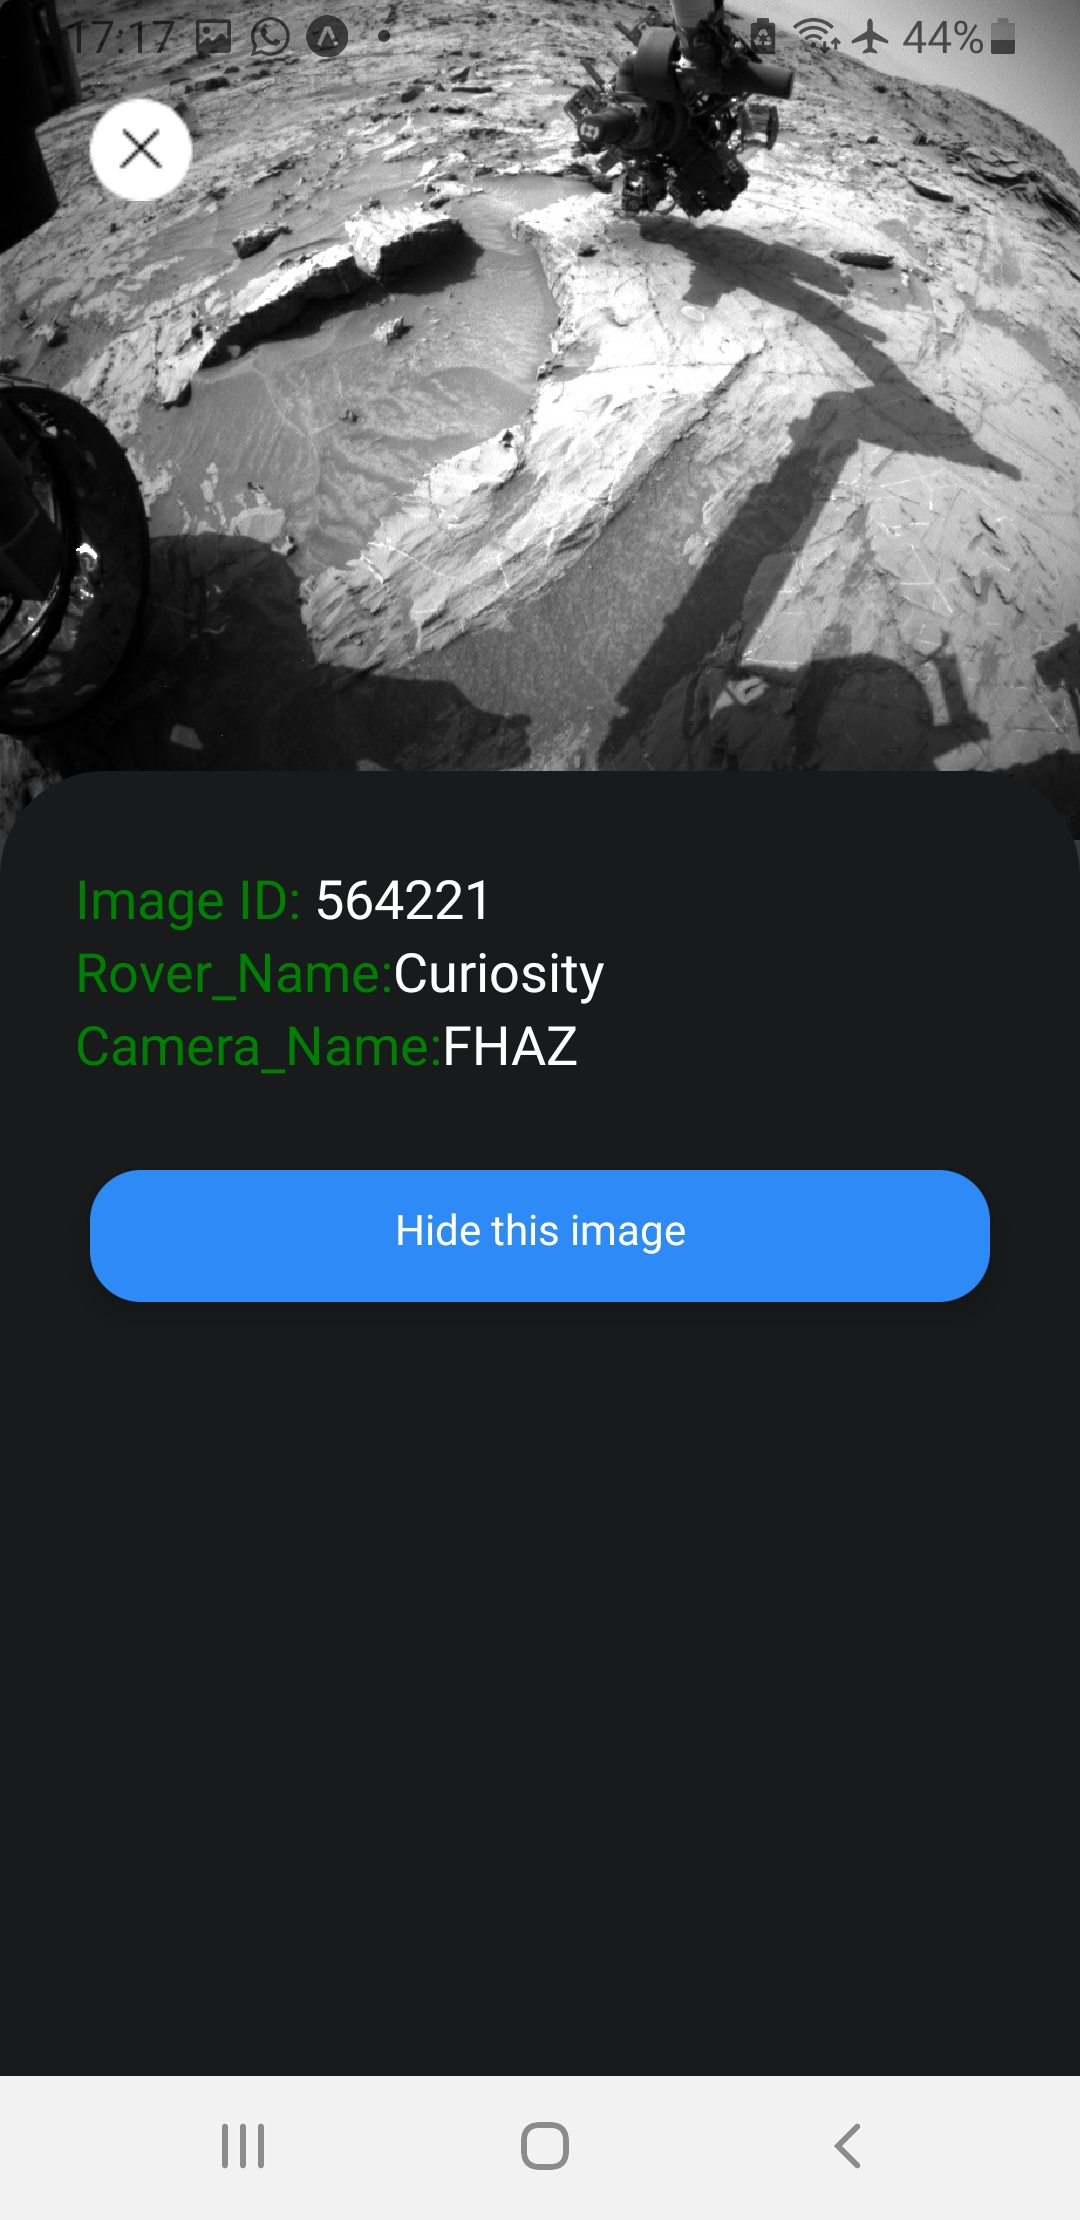
\includegraphics[width=5cm, height=10cm]{images/immaginiAndroid/imageDetail.jpg}
        \caption{\label{imageDetailAndroid} Android dettagli immagine}
    \end{minipage}
    \hfill
    \begin{minipage}[h]{0.47\textwidth}
        \centering
        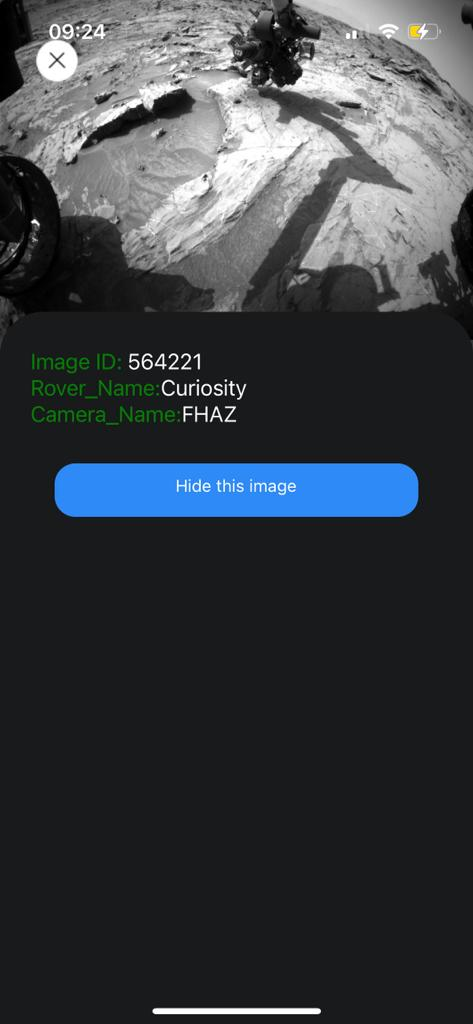
\includegraphics[width=5cm, height=10cm]{images/immaginiPhone/imageDetail.jpeg}
        \caption{\label{imageDetailIphone}iPhone dettagli immagine}
    \end{minipage}
\end{figure}

\section{Filtri Photos e Hide All}
Una volta nascoste le immagini, queste non vengono mostrate all'utente quando effettua una ricerca: possono per\`o essere ripristinate tramite l'utilizzo del filtro ``Photos".
Nella Fig 4.15 si pu\`o notare che l'immagine con ID=564234 non \`e visibile prima di premere il pulsante ``Photos"; questa viene visualizzata dopo averlo premuto.

All'utente viene fornita la possibilit\`a di nascondere tutti gli elementi di una ricerca premendo il pulsante ``Hide All".
\begin{figure}[h]
    \begin{minipage}[h]{0.47\textwidth}
        \centering
        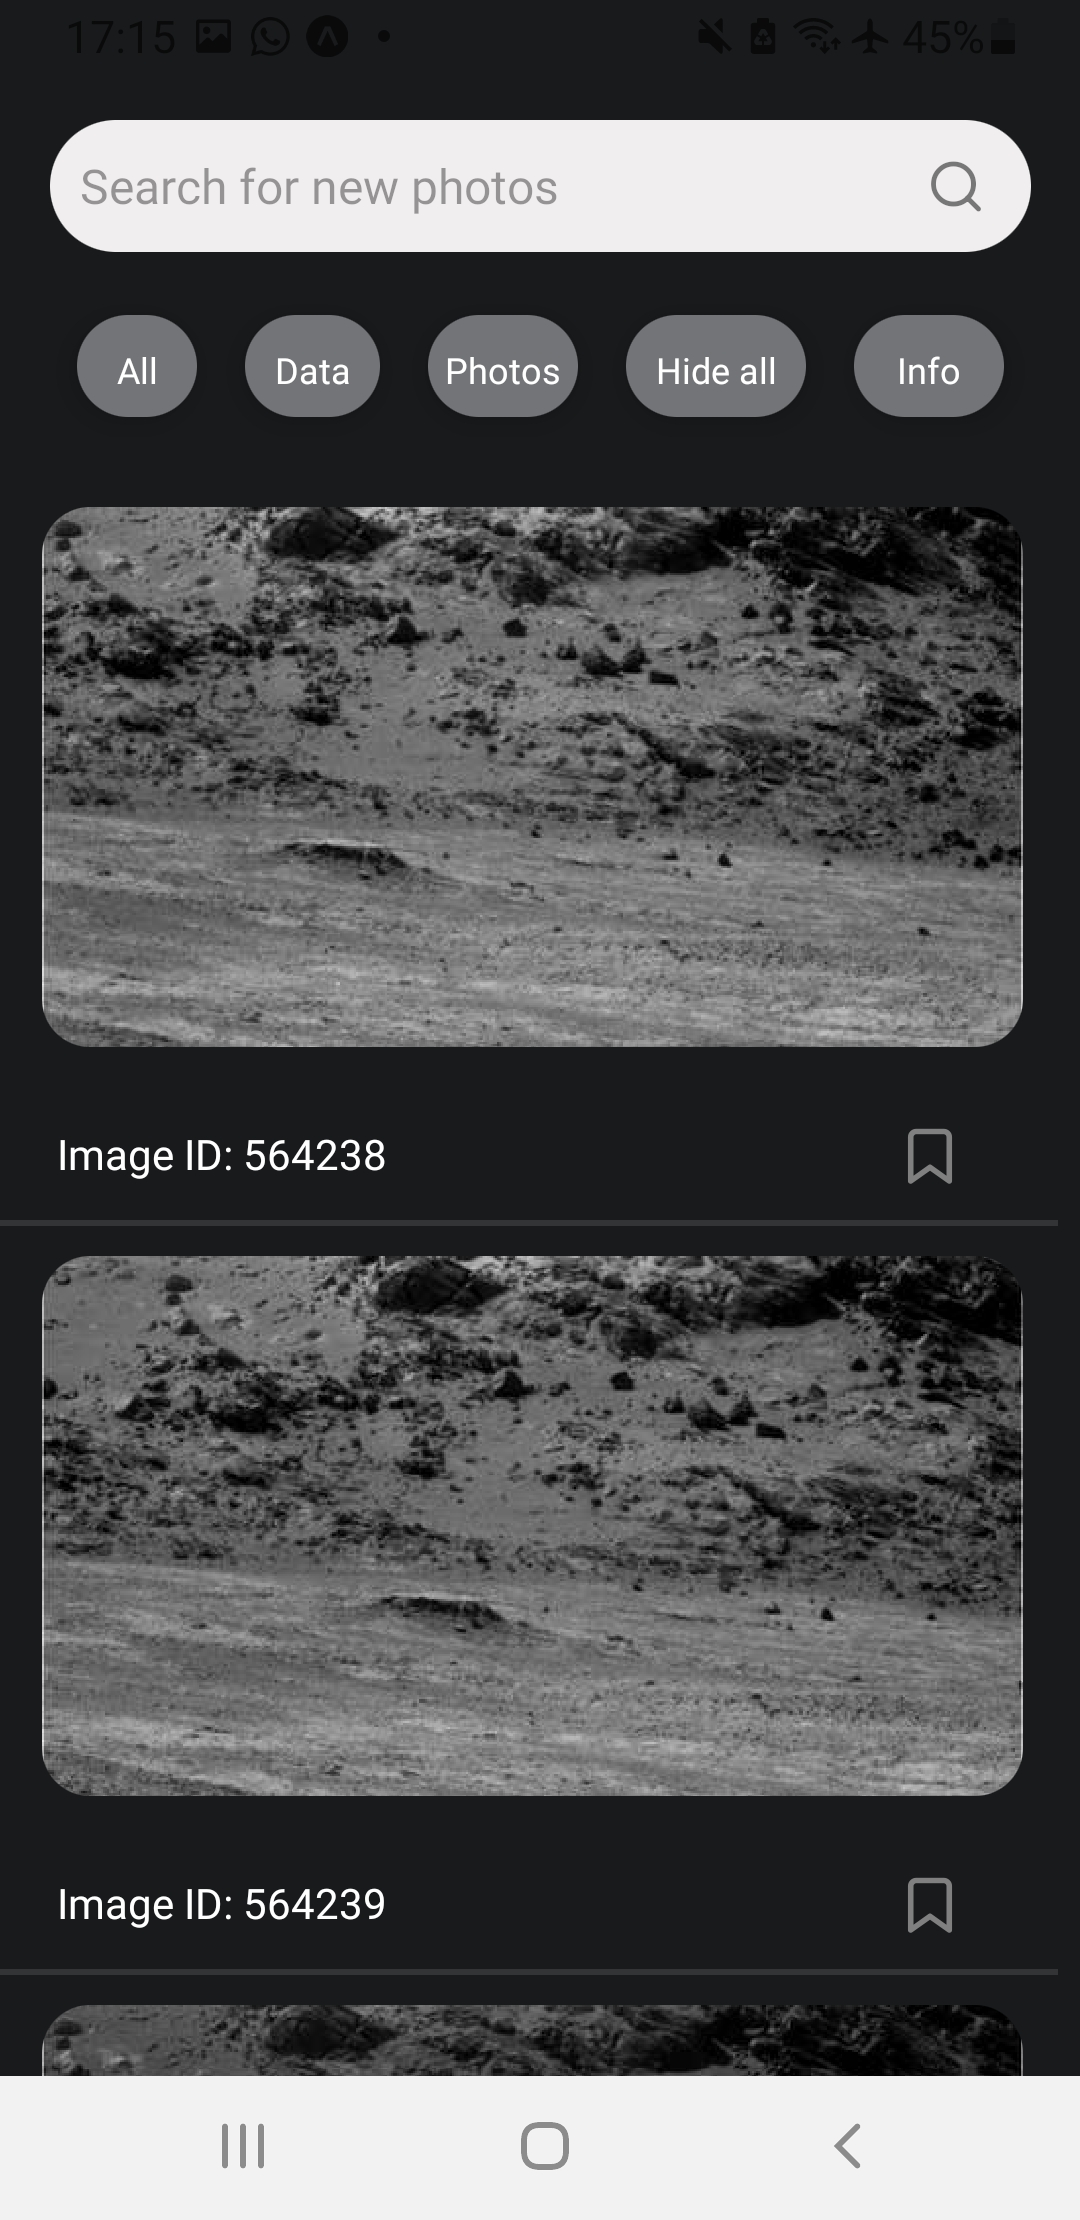
\includegraphics[width=5cm, height=10cm]{images/immaginiAndroid/prePhotos.jpg}
        \caption{\label{prePhotosAndroid} Lista delle immagini prima di usare il filtro Photos}
    \end{minipage}
    \hfill
    \begin{minipage}[h]{0.47\textwidth}
        \centering
        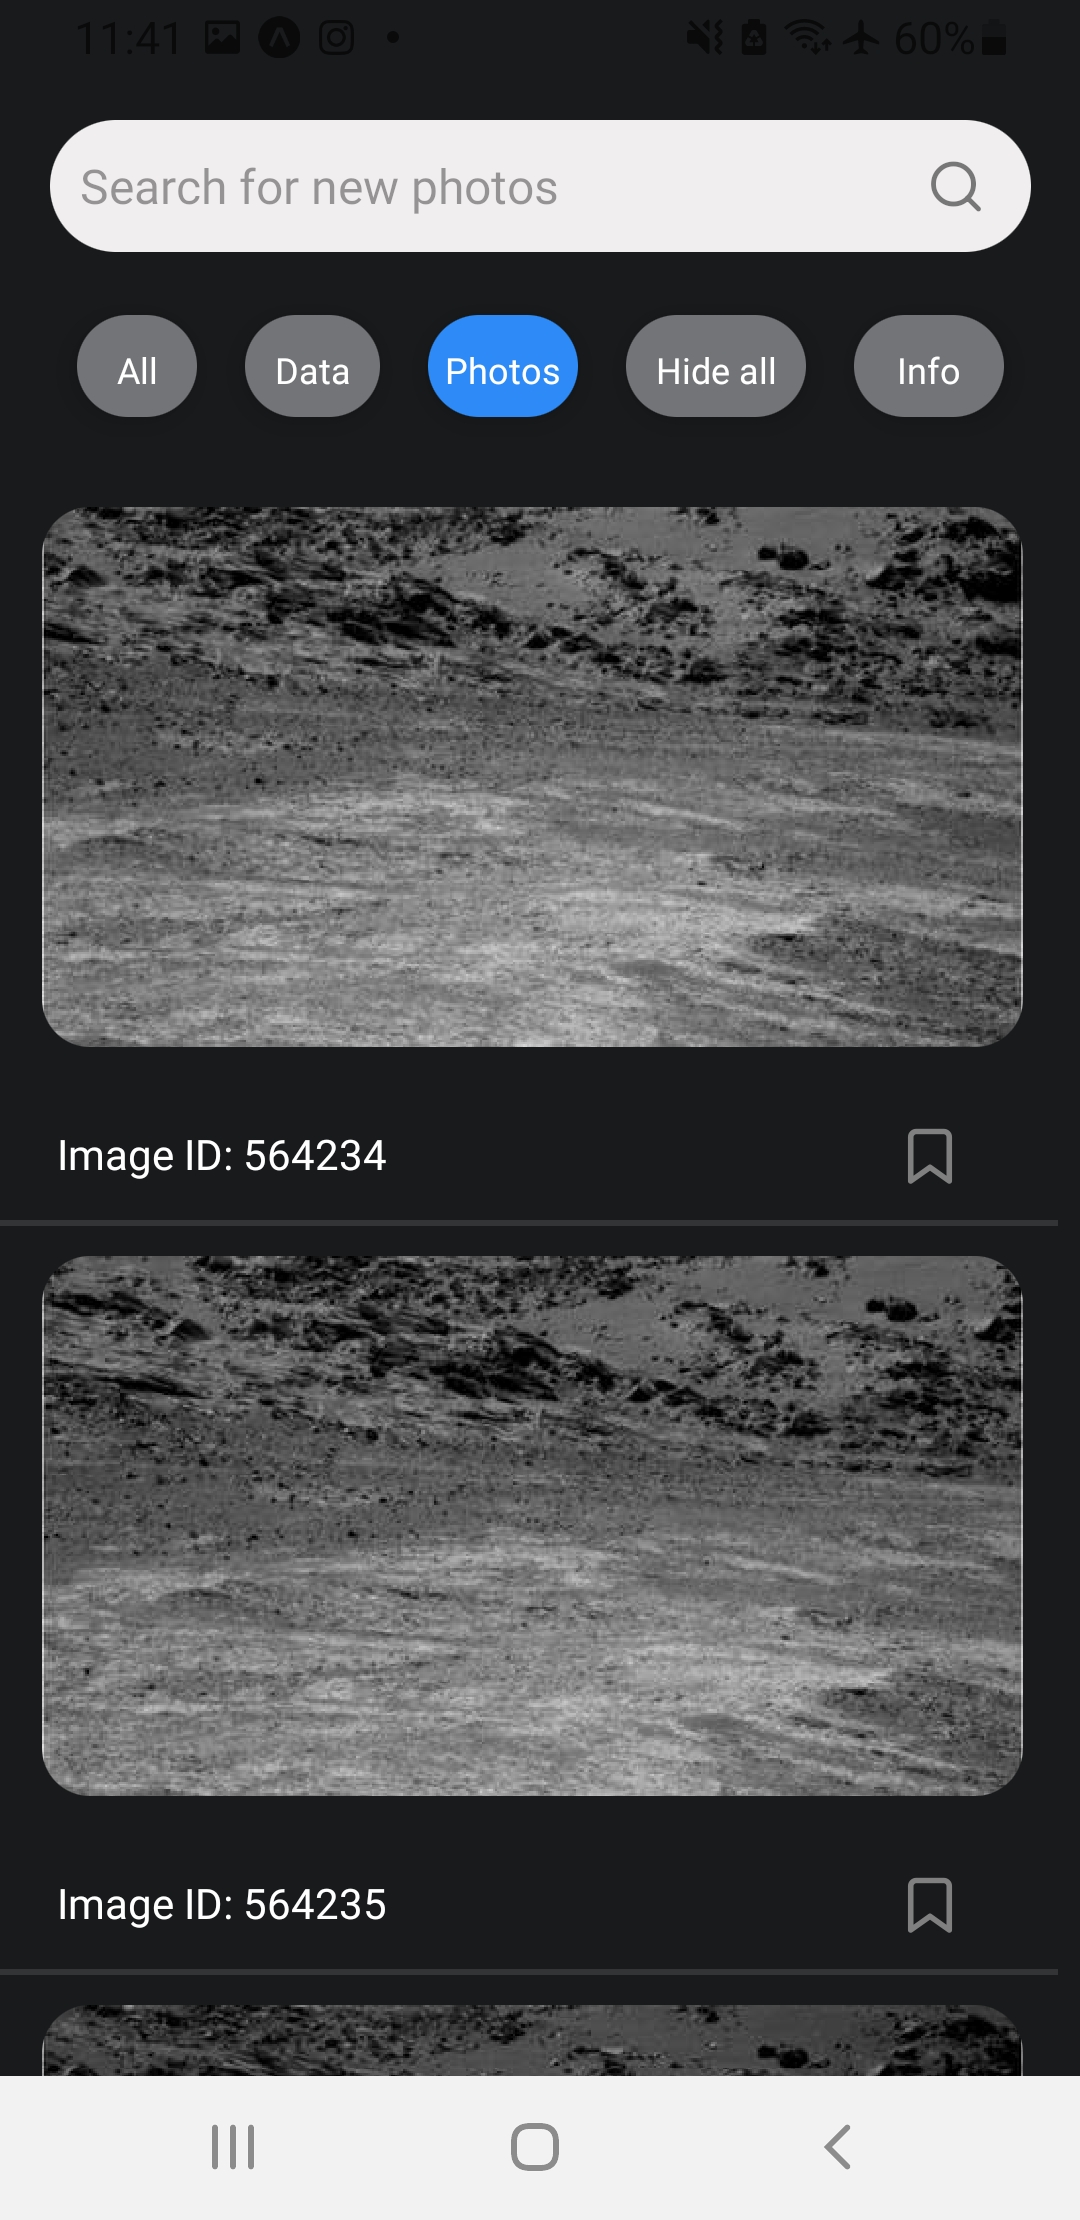
\includegraphics[width=5cm, height=10cm]{images/immaginiAndroid/postPhotos.jpg}
        \caption{\label{postPhotosAndroid} Lista delle immagini dopo l'uso del filtro Photos}
    \end{minipage}
\end{figure}
\section{Parametri di Ricerca Errati}
Quando l'utente effettua una nuova ricerca di immagini, potrebbe inserire dei parametri di ricerca errati come ad esempio il nome del Rover errato e la data solare in formato errato;
in tal caso nessuna immagine viene recuperata. In queste situazioni l'applicativo si occupa di informare l'utente del fatto che nessuna immagine \`e
stata trovata e viene visualizzata a schermo una lista vuota.

Osservando le Fig 4.17 e 4.18 possiamo notare che le visualizzazione delle modali non cambia tra Android e iOS; l'unica differenza percepibile nei due dispositivi consiste in un testo pi\`u marcato in Android.
\begin{figure}[h]
    \begin{minipage}[h]{0.47\textwidth}
        \centering
        \includegraphics[width=5cm, height=10cm]{images/immaginiAndroid/ricercaErrata.jpg}
        \caption{\label{ricercaErrataAndroid} Android ricerca errata}
    \end{minipage}
    \hfill
    \begin{minipage}[h]{0.47\textwidth}
        \centering
        \includegraphics[width=5cm, height=10cm]{images/immaginiPhone/ricercaErrata.jpeg}
        \caption{\label{ricercaErrataIphone} iPhone ricerca errata}
    \end{minipage}
\end{figure}

\section{Animazione Onde Gravitazionali}
Ogni volta che viene eseguita una nuova ricerca, dopo aver premuto il pulsante ``All", viene avviata una animazione. In questo modo l'utente ha una migliore UX (User Experience) in quanto viene informato che la ricerca \`e inziziata e l'animazione ricorda le onde gravitazionali, quindi lo spazio.
\begin{figure}[H]
    \begin{minipage}[h]{0.47\textwidth}
        \centering
        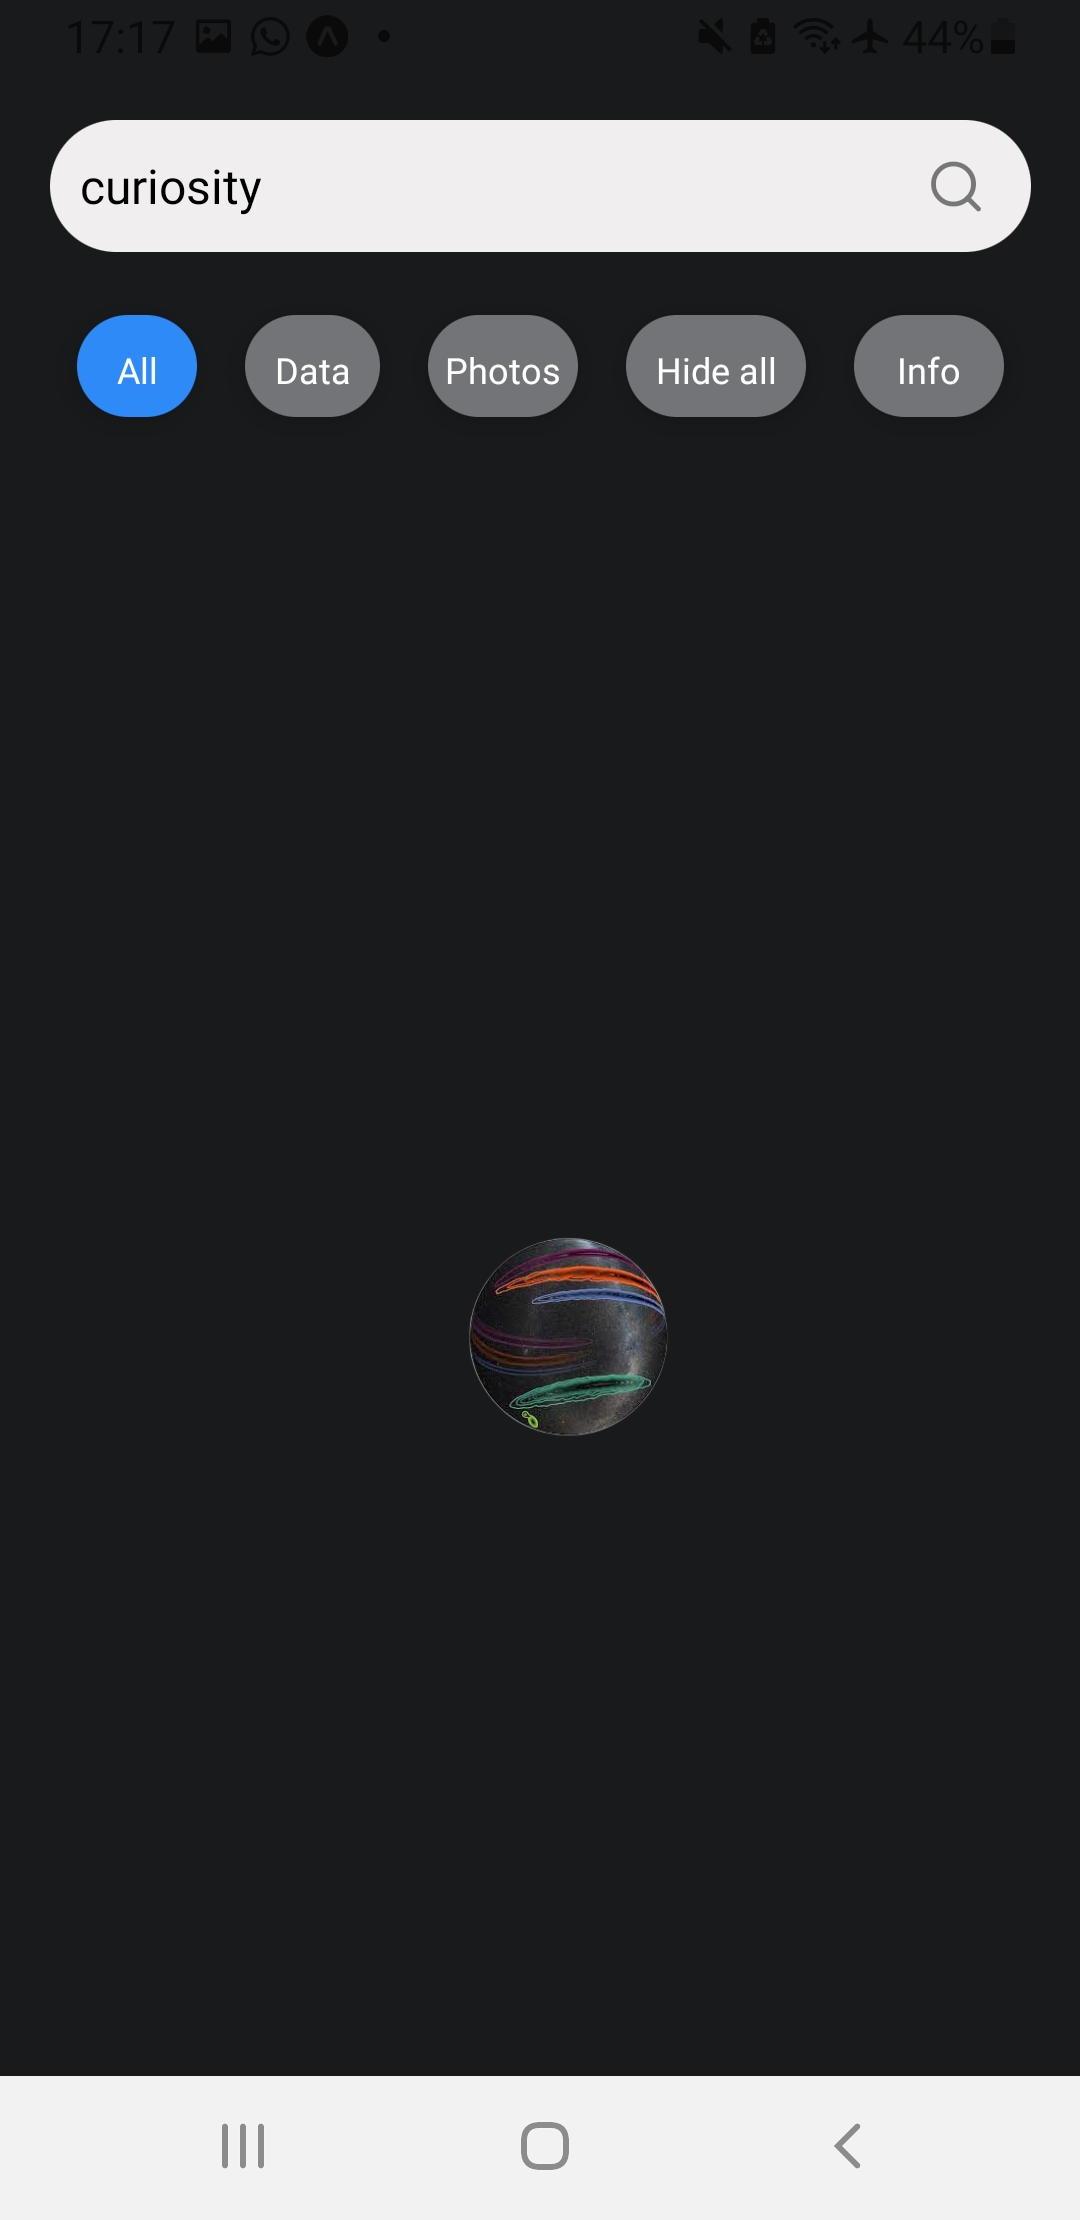
\includegraphics[width=5cm, height=10cm]{images/immaginiAndroid/animazione.jpg}
        \caption{\label{animazioneAndroid} Android animazione onde gravitazionali}
    \end{minipage}
    \hfill
    \begin{minipage}[h]{0.47\textwidth}
        \centering
        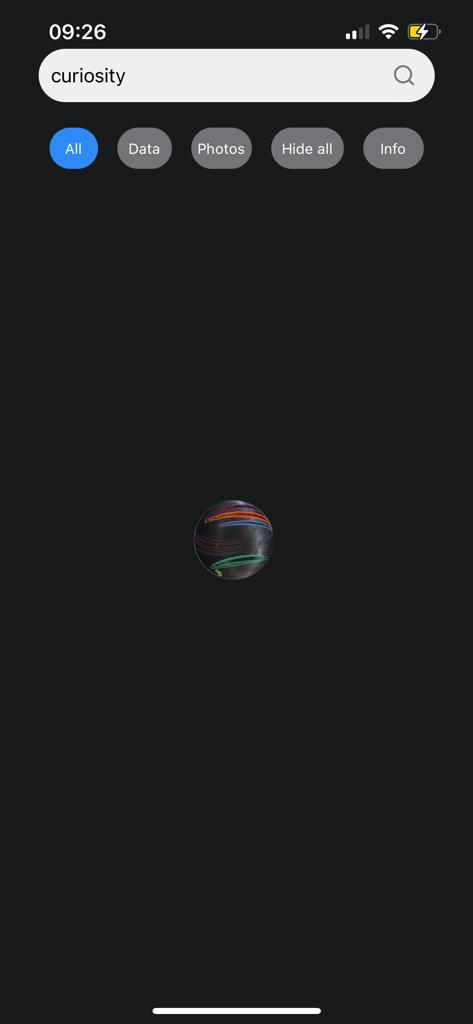
\includegraphics[width=5cm, height=10cm]{images/immaginiPhone/animazione.jpeg}
        \caption{\label{animazioneIphone} iPhone animazione onde gravitazionali}
    \end{minipage}
\end{figure}

\section{Istruzioni sui Metodi di Ricerca}
Affinch\`e l'utente possa utilizzare correttamente l'applicazione, nello screen principale e in quello dedicato alla ricerca per data solare, sono state inserite dello icone ``info-point".
Queste ultime se premute mostrano delle modali che istruiscono l'utente sul corretto uso dell'applicativo. Come gi\`a detto in precendenza la presentazione visiva delle modali non cambia tra iOS e Android.
\begin{figure}[H]
    \begin{minipage}[h]{0.47\textwidth}
        \centering
        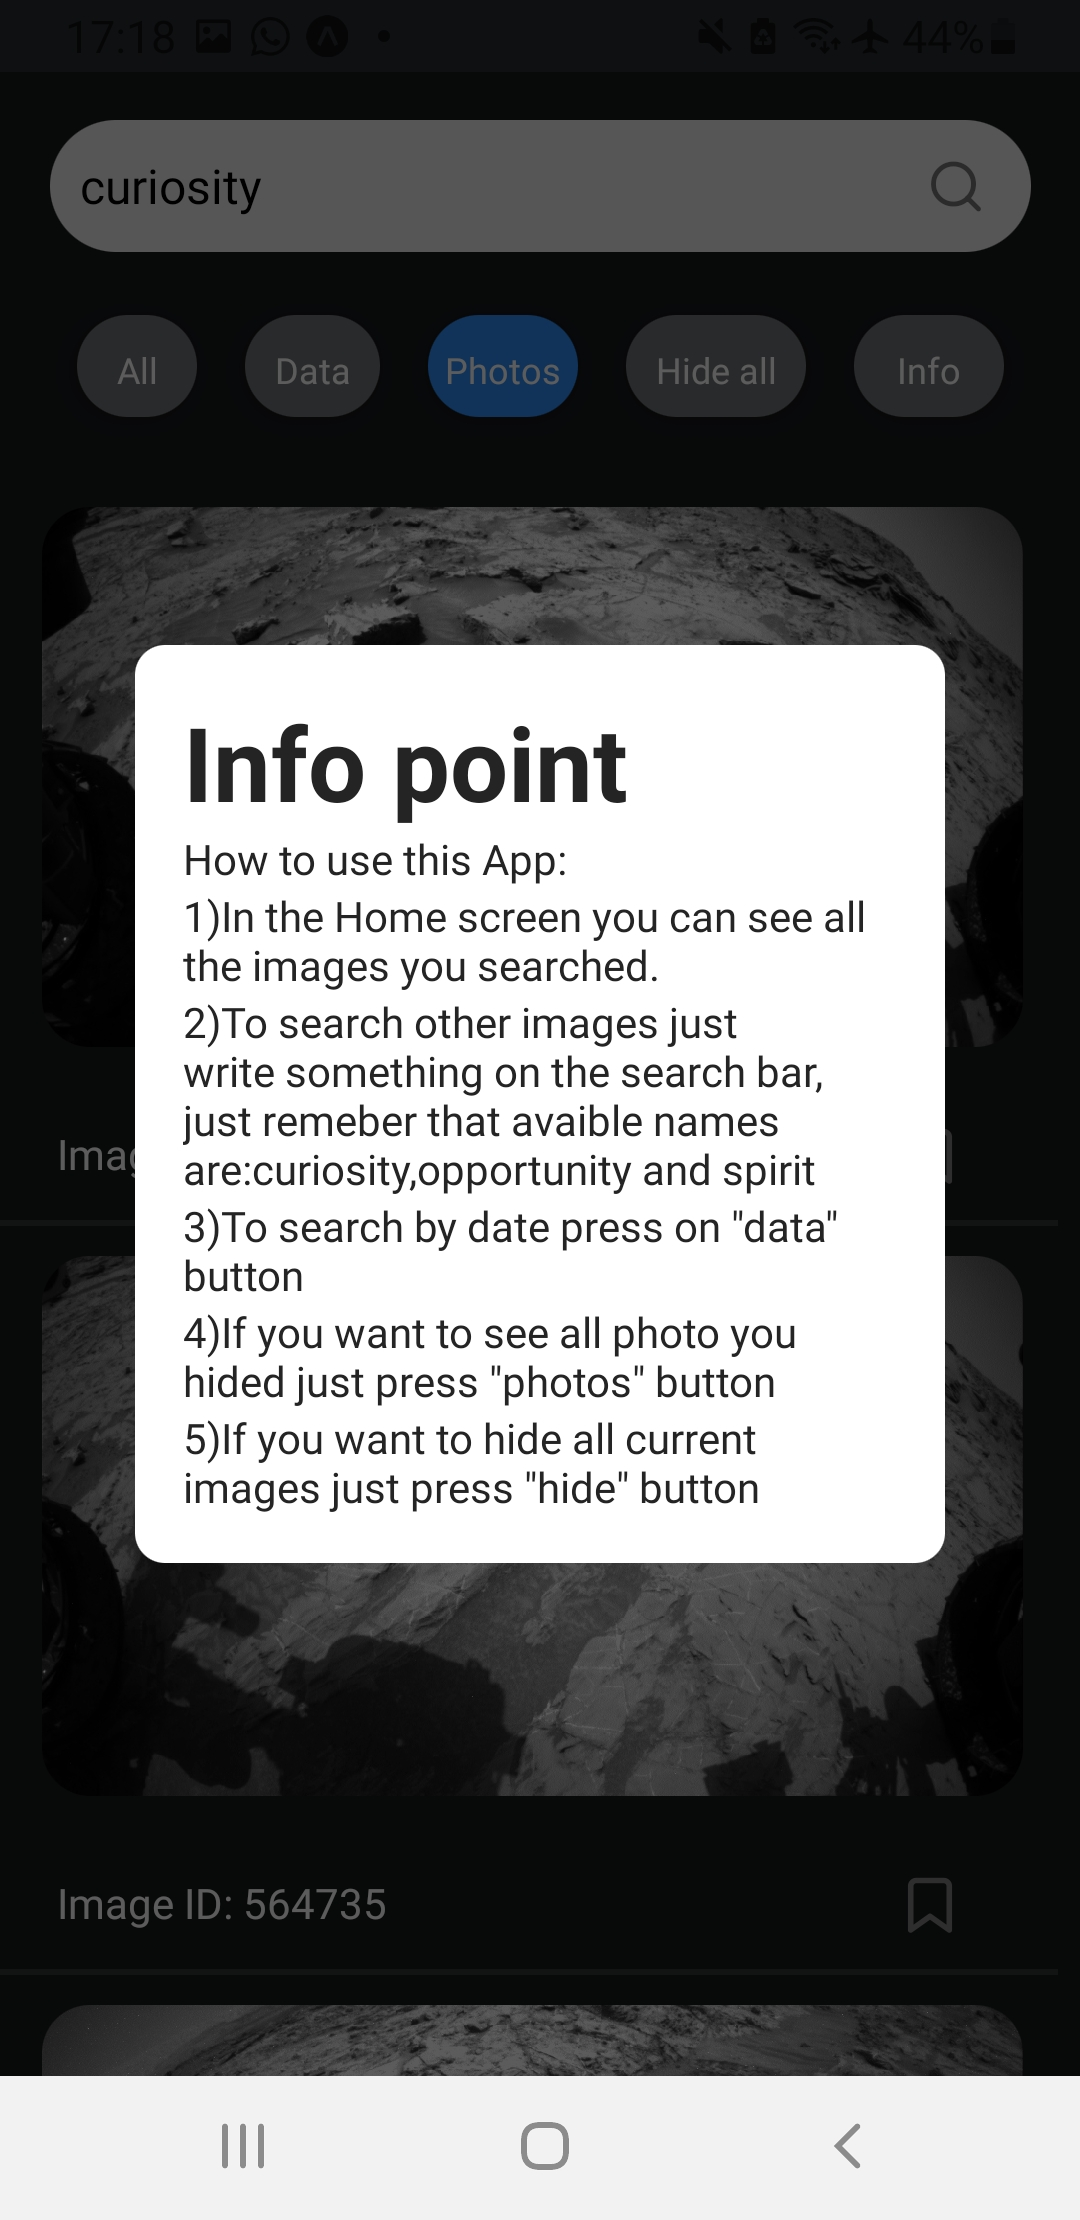
\includegraphics[width=5cm, height=10cm]{images/immaginiAndroid/infoPoint.jpg}
        \caption{\label{infoPointAndroid} Android info-point}
    \end{minipage}
    \hfill
    \begin{minipage}[h]{0.47\textwidth}
        \centering
        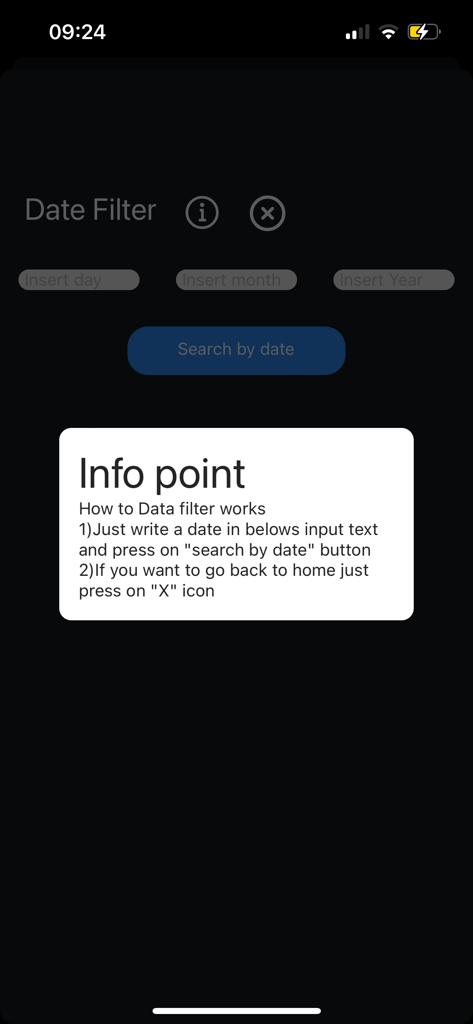
\includegraphics[width=5cm, height=10cm]{images/immaginiPhone/infoPoint.jpeg}
        \caption{\label{infoPointIphone} iPhone info-point}
    \end{minipage}
\end{figure}

\section{Procedura di Logout}
Per effettuare il logout dal proprio profilo, l'utente deve scorrere le immagini fino alla fine della lista e premere sul pulsante ``Log out". Una volta fatto ci\`o si viene reindirizzati alla schermata di \textit{sign in} o \textit{sign up}.

Nelle Fig 4.23 e 4.24 si pu\`o vedere che in Android si ha una migliore User Experience, in quanto il pulsante di logout non si soprappone ad altri componenti nativi del dispositivo: ad esempio sull'iPhone la barra orizzontale in fondo allo schermo si sovrappone al pulsante di Log out
\begin{figure}[H]
    \begin{minipage}[h]{0.47\textwidth}
        \centering
        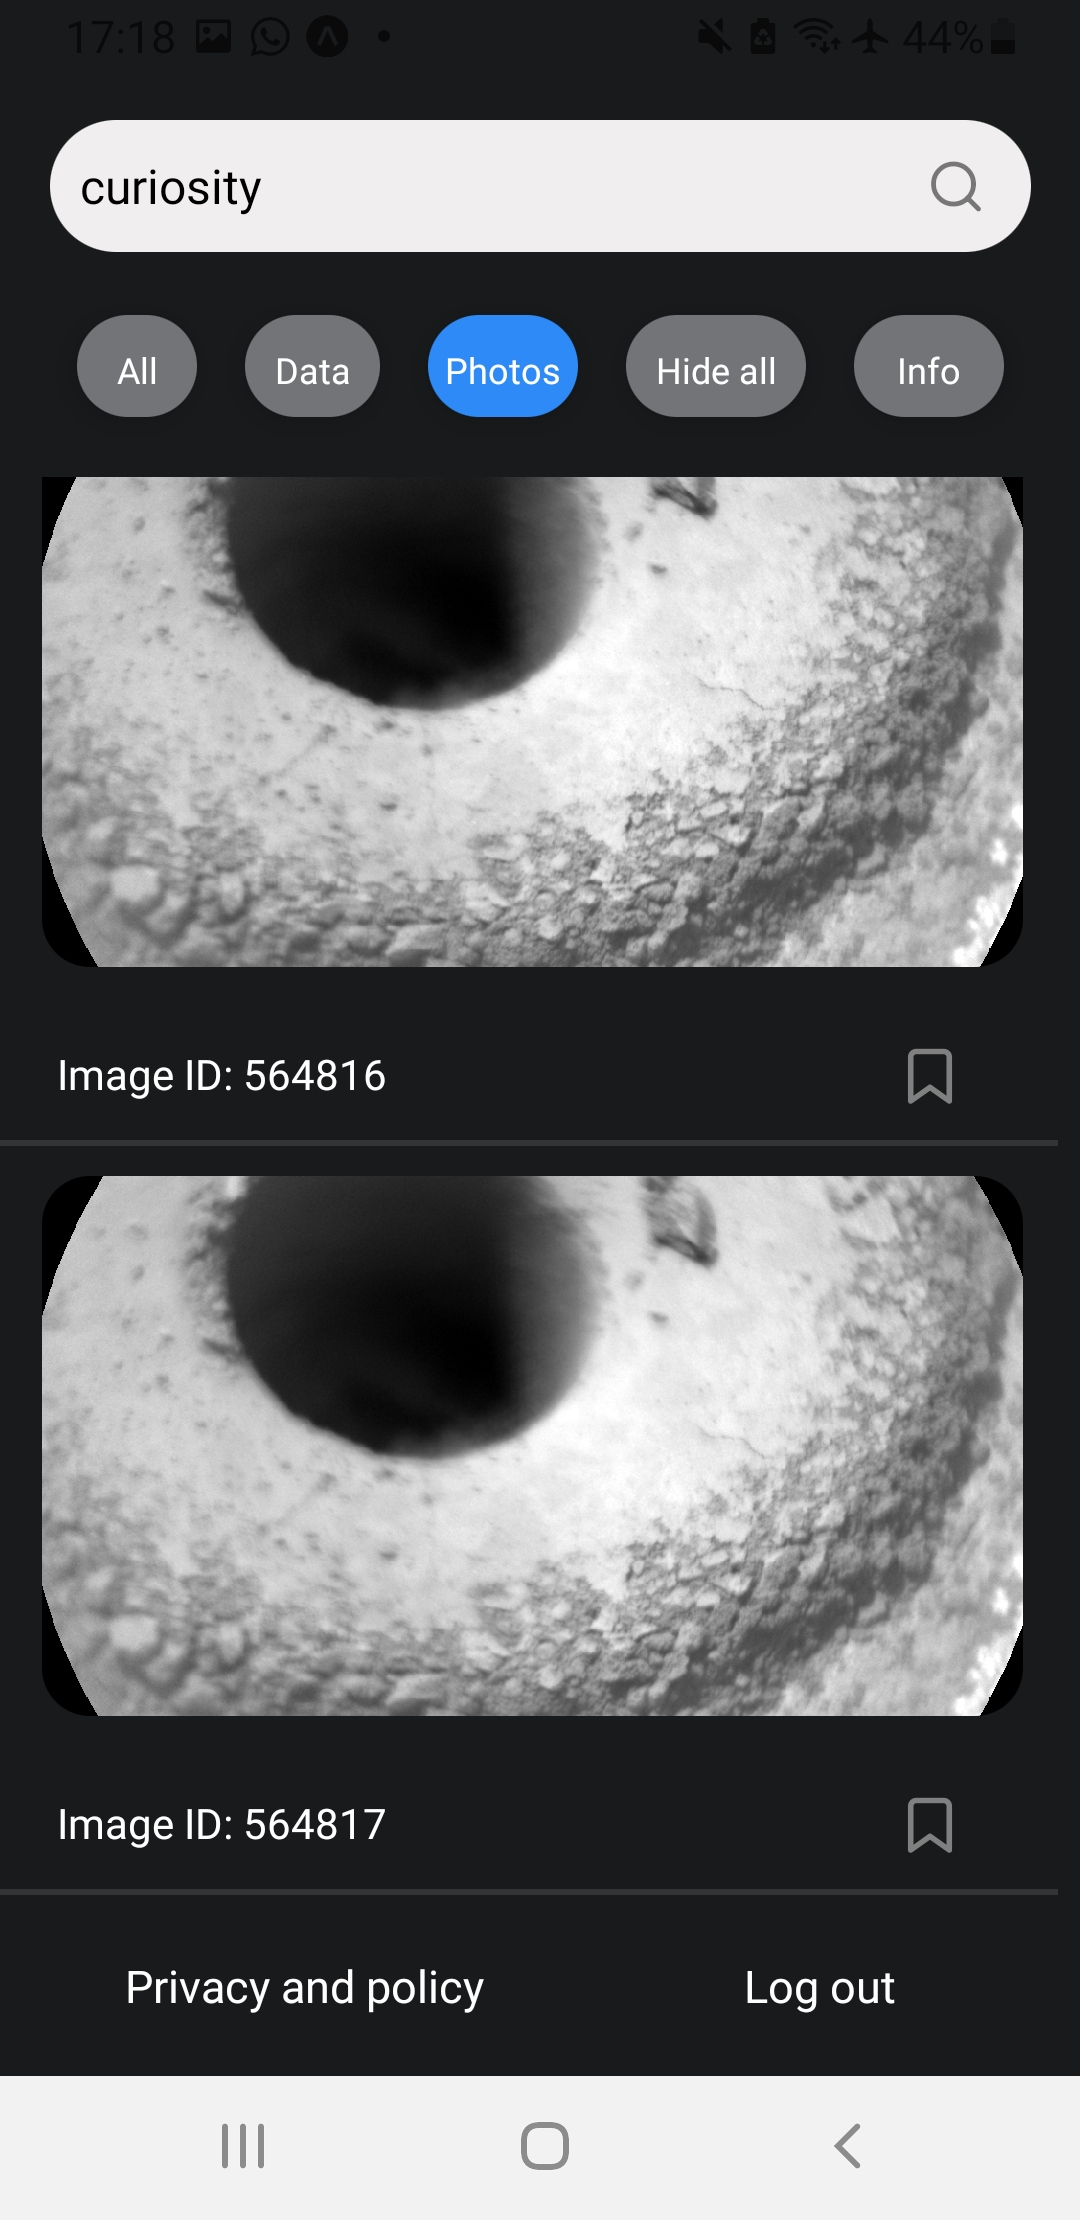
\includegraphics[width=5cm, height=10cm]{images/immaginiAndroid/logout.jpg}
        \caption{\label{logoutAndroid} Android pulsante di logout}
    \end{minipage}
    \hfill
    \begin{minipage}[h]{0.47\textwidth}
        \centering
        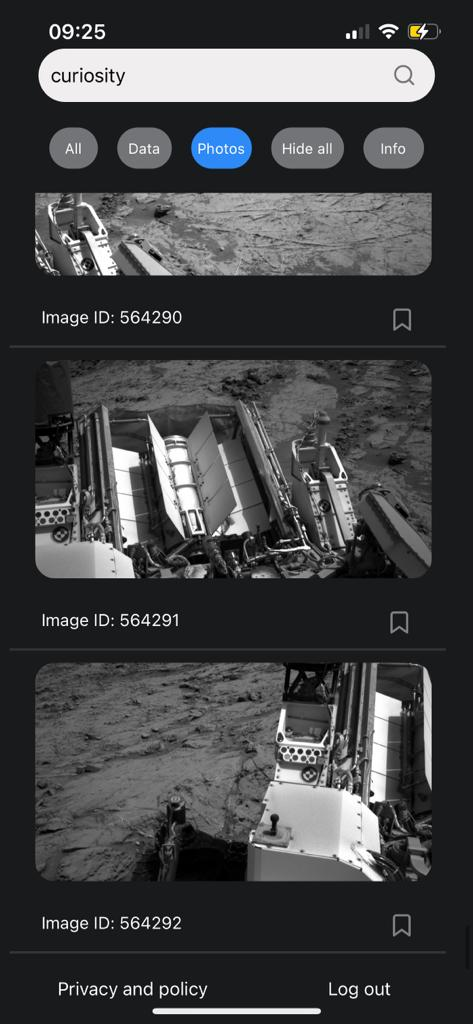
\includegraphics[width=5cm, height=10cm]{images/immaginiPhone/logout.jpeg}
        \caption{\label{logoutIphone} iPhone pulsante di logout}
    \end{minipage}
\end{figure}


\clearpage

\chapter*{Conclusioni}
% \chapter* -> the introduction isn't the Chapter 1, it's not a numbered chapter
\addcontentsline{toc}{chapter}{Conclusioni} % this line enable the introduction to be listed in the Table Of Contents even if it's not a numbered chapter (see above)
\markboth{}{}

In questo capitolo verranno discussi gli obiettivi, i risultati e le conoscenze acquisite al termine del tirocinio ed eventuali sviluppi futuri dell'applicazione.

\section{Obiettivi e Risultati Raggiunti}
Gli obiettivi principali di questo progetto di tirocinio sono stati:
\begin{enumerate}
    \item Lo sviluppo di un'applicazione multipiattaforma, quindi di un applicativo che possa funzionare su diversi sistemi operativi.
    \item L'uso del protocollo HTTP per la comunicazione con i server della Nasa.
    \item L'utilizzo del formato JSON per la trasmissione e l'estrapolazione di dati.
    \item La gestione della navigazione tra i vari screen dell'applicazione.
    \item La comprensione e l'utilizzo dell'architettura modulare.
\end{enumerate}

Tutti questi obiettivi non solo sono stati raggiunti con successo, ma \`e stato aggiunto anche uno strato di autenticazione e registrazione che non era richiesto dal progetto.
Come si pu\`o dedurre dal capitolo ``RISULTATI", il primo obiettivo \`e stato raggiunto in pieno: l'applicazione svolge le stesse funzioni sia su Android che iOS. Nonostante ci\`o, essendo stato
utilizzato lo stesso codice per entrambe le piattaforme, vi saranno sempre delle differenze per quanto riguarda gli aspetti grafici. L'applicazione non presenta
cali di performance, il che dimostra che lo sviluppo di applicazioni multipiattaforma \`e una valida alternativa allo sviluppo nativo.
Si sottolinea che questo applicativo non fa uso di funzioni native del dispositivo come GPS e notifiche Push.

Sia il secondo che il terzo obiettivo sono stati raggiunti con successo: dal capitolo ``IMPLEMENTAZIONE" si pu\`o infatti osservare che ad ogni ricerca vengono caricate delle nuove immagini, e questo \`e il risultato
di diverse richieste HTTP. Inoltre l'uso del formato JSON per la trasmissione dei dati \`e stato cruciale: in effetti le immagini restituite dai server della Nasa sono proprio in questo formato. Tramite JSON \`e stato possibile comunicare facilmente al server locale
le credenziali inserite da ogni utente e in seguito estrarre il JWT dalle risposte ottenute.

Durante l'utilizzo dell'applicazione, la navigazione tra i vari screen che la compongono risulta essere fluida e garantisce una buona UX. Nonostante ci\`o,
essendo l'applicazione multipiattaforma, la navigazione pu\`o essere diversa tra i vari sistemi operativi a causa delle funzioni navigazione nativa di ogni dispositivo.

Oltre a poter testare l'applicazione in locale ne \`e stata fatta anche la build in modo da poterla distribuire sugli store in un futuro, a seguito di ulteriori migliorie.
La build \`e stata caricata sul sito di Expo ed \`e possibile scaricarne l'apk.

\section{Conoscenze Acquisite}
Terminato il progetto si pu\`o dire di aver approfondito ed acqusisto competenze con nuovi strumenti e tecnologie, in particolare:
\begin{itemize}
    \item JavaScript: l'utilizzo di JavaScript al di fuori dello sviluppo web \`e stato particolarme utile per capire come utilizzare questo linguaggio sia per lo sviluppo
          lato server, tramite Node.js, sia per lo sviluppo dell'intera applicazione tramite l'utilizzo del framework React Native.
    \item Expo: il suo utilizzo ha permesso di iniziare lo sviluppo dell'applicazione fin da subito e lasciare la gestione di eventuali altre attivit\`a a servizi di terze parti. Questo strumento \`e
          una perfetta scelta per l'introduzione allo sviluppo mobile.
    \item Node.js: attraverso la realizzazione di questo applicativo \`e stato possibile approfondire l'utilizzo di JavaScript nello sviluppo lato server, e comprendere meglio l'importanza delle API.
    \item Mongodb: questo database NoSQL \`e stata una scelta necessaria, in quanto il server locale e l'applicazione comunicano attraverso il formato JSON. Nonostante ci\`o, \`e stato molto interessante
          e utile imparare la logica di comunicazione e memorizzazione di un database NoSQL.
\end{itemize}

\section{Sviluppi Futuri}
Nonostante l'applicazione soddisfi tutti i requisiti di progetto, si potrebbe pensare di aggiungere altre funzionalit\`a come:
\begin{itemize}
    \item La possibilit\`a di ricercare le immagini in base alla camera utilizzata per scattare le foto.
    \item La possibilit\`a di ricercare le immagini per data ``Marziana".
\end{itemize}
Un altro possibile miglioramento potrebbe consistere nel memorizzare le ultime immagini visualizzate dall'utente sul database, piuttosto che mantenerle in modo persistente sul dispositivo: in questo
modo si risparmierebbe memoria.
Per garantire una migliore UX si potrebbe creare una classifica delle immagini pi\`u visualizzate: in questo modo ogni utente potrebbe dare la propria opinione sulle diverse immagini. In base a questa
classifica si potrebbe decidere di non mostrare le immagini meno popolari.

\clearpage

\appendix
\renewcommand{\chaptermark}[1]{\markboth{{\appendixname}\ \thechapter.\hspace{1em}#1}{}}

%\chapter{Appendice}



\clearpage

\addcontentsline{toc}{chapter}{Bibliografia}
\bibliographystyle{unsrt}
\nocite{*}
\bibliography{riferimenti}
% 
\clearpage

\end{document}


